


\documentclass[conference]{IEEEtran}
% Some Computer Society conferences also require the compsoc mode option,
% but others use the standard conference format.
%
% If IEEEtran.cls has not been installed into the LaTeX system files,
% manually specify the path to it like:
% \documentclass[conference]{../sty/IEEEtran}

\usepackage[utf8]{inputenc}
\usepackage{graphicx}
\usepackage{amsmath}
\usepackage{url}
\usepackage{algorithm} 
\usepackage{algpseudocode} 
\usepackage{caption}
\usepackage{subcaption}
\usepackage{float}
% Some very useful LaTeX packages include:
% (uncomment the ones you want to load)


% *** MISC UTILITY PACKAGES ***
%
%\usepackage{ifpdf}
% Heiko Oberdiek's ifpdf.sty is very useful if you need conditional
% compilation based on whether the output is pdf or dvi.
% usage:
% \ifpdf
%   % pdf code
% \else
%   % dvi code
% \fi
% The latest version of ifpdf.sty can be obtained from:
% http://www.ctan.org/pkg/ifpdf
% Also, note that IEEEtran.cls V1.7 and later provides a builtin
% \ifCLASSINFOpdf conditional that works the same way.
% When switching from latex to pdflatex and vice-versa, the compiler may
% have to be run twice to clear warning/error messages.






% *** CITATION PACKAGES ***
%
%\usepackage{cite}
% cite.sty was written by Donald Arseneau
% V1.6 and later of IEEEtran pre-defines the format of the cite.sty package
% \cite{} output to follow that of the IEEE. Loading the cite package will
% result in citation numbers being automatically sorted and properly
% "compressed/ranged". e.g., [1], [9], [2], [7], [5], [6] without using
% cite.sty will become [1], [2], [5]--[7], [9] using cite.sty. cite.sty's
% \cite will automatically add leading space, if needed. Use cite.sty's
% noadjust option (cite.sty V3.8 and later) if you want to turn this off
% such as if a citation ever needs to be enclosed in parenthesis.
% cite.sty is already installed on most LaTeX systems. Be sure and use
% version 5.0 (2009-03-20) and later if using hyperref.sty.
% The latest version can be obtained at:
% http://www.ctan.org/pkg/cite
% The documentation is contained in the cite.sty file itself.






% *** GRAPHICS RELATED PACKAGES ***
%
\ifCLASSINFOpdf
  % \usepackage[pdftex]{graphicx}
  % declare the path(s) where your graphic files are
  % \graphicspath{{../pdf/}{../jpeg/}}
  % and their extensions so you won't have to specify these with
  % every instance of \includegraphics
  % \DeclareGraphicsExtensions{.pdf,.jpeg,.png}
\else
  % or other class option (dvipsone, dvipdf, if not using dvips). graphicx
  % will default to the driver specified in the system graphics.cfg if no
  % driver is specified.
  % \usepackage[dvips]{graphicx}
  % declare the path(s) where your graphic files are
  % \graphicspath{{../eps/}}
  % and their extensions so you won't have to specify these with
  % every instance of \includegraphics
  % \DeclareGraphicsExtensions{.eps}
\fi
% graphicx was written by David Carlisle and Sebastian Rahtz. It is
% required if you want graphics, photos, etc. graphicx.sty is already
% installed on most LaTeX systems. The latest version and documentation
% can be obtained at: 
% http://www.ctan.org/pkg/graphicx
% Another good source of documentation is "Using Imported Graphics in
% LaTeX2e" by Keith Reckdahl which can be found at:
% http://www.ctan.org/pkg/epslatex
%
% latex, and pdflatex in dvi mode, support graphics in encapsulated
% postscript (.eps) format. pdflatex in pdf mode supports graphics
% in .pdf, .jpeg, .png and .mps (metapost) formats. Users should ensure
% that all non-photo figures use a vector format (.eps, .pdf, .mps) and
% not a bitmapped formats (.jpeg, .png). The IEEE frowns on bitmapped formats
% which can result in "jaggedy"/blurry rendering of lines and letters as
% well as large increases in file sizes.
%
% You can find documentation about the pdfTeX application at:
% http://www.tug.org/applications/pdftex





% *** MATH PACKAGES ***
%
%\usepackage{amsmath}
% A popular package from the American Mathematical Society that provides
% many useful and powerful commands for dealing with mathematics.
%
% Note that the amsmath package sets \interdisplaylinepenalty to 10000
% thus preventing page breaks from occurring within multiline equations. Use:
%\interdisplaylinepenalty=2500
% after loading amsmath to restore such page breaks as IEEEtran.cls normally
% does. amsmath.sty is already installed on most LaTeX systems. The latest
% version and documentation can be obtained at:
% http://www.ctan.org/pkg/amsmath





% *** SPECIALIZED LIST PACKAGES ***
%
%\usepackage{algorithmic}
% algorithmic.sty was written by Peter Williams and Rogerio Brito.
% This package provides an algorithmic environment fo describing algorithms.
% You can use the algorithmic environment in-text or within a figure
% environment to provide for a floating algorithm. Do NOT use the algorithm
% floating environment provided by algorithm.sty (by the same authors) or
% algorithm2e.sty (by Christophe Fiorio) as the IEEE does not use dedicated
% algorithm float types and packages that provide these will not provide
% correct IEEE style captions. The latest version and documentation of
% algorithmic.sty can be obtained at:
% http://www.ctan.org/pkg/algorithms
% Also of interest may be the (relatively newer and more customizable)
% algorithmicx.sty package by Szasz Janos:
% http://www.ctan.org/pkg/algorithmicx




% *** ALIGNMENT PACKAGES ***
%
%\usepackage{array}
% Frank Mittelbach's and David Carlisle's array.sty patches and improves
% the standard LaTeX2e array and tabular environments to provide better
% appearance and additional user controls. As the default LaTeX2e table
% generation code is lacking to the point of almost being broken with
% respect to the quality of the end results, all users are strongly
% advised to use an enhanced (at the very least that provided by array.sty)
% set of table tools. array.sty is already installed on most systems. The
% latest version and documentation can be obtained at:
% http://www.ctan.org/pkg/array


% IEEEtran contains the IEEEeqnarray family of commands that can be used to
% generate multiline equations as well as matrices, tables, etc., of high
% quality.




% *** SUBFIGURE PACKAGES ***
%\ifCLASSOPTIONcompsoc
%  \usepackage[caption=false,font=normalsize,labelfont=sf,textfont=sf]{subfig}
%\else
%  \usepackage[caption=false,font=footnotesize]{subfig}
%\fi
% subfig.sty, written by Steven Douglas Cochran, is the modern replacement
% for subfigure.sty, the latter of which is no longer maintained and is
% incompatible with some LaTeX packages including fixltx2e. However,
% subfig.sty requires and automatically loads Axel Sommerfeldt's caption.sty
% which will override IEEEtran.cls' handling of captions and this will result
% in non-IEEE style figure/table captions. To prevent this problem, be sure
% and invoke subfig.sty's "caption=false" package option (available since
% subfig.sty version 1.3, 2005/06/28) as this is will preserve IEEEtran.cls
% handling of captions.
% Note that the Computer Society format requires a larger sans serif font
% than the serif footnote size font used in traditional IEEE formatting
% and thus the need to invoke different subfig.sty package options depending
% on whether compsoc mode has been enabled.
%
% The latest version and documentation of subfig.sty can be obtained at:
% http://www.ctan.org/pkg/subfig




% *** FLOAT PACKAGES ***
%
%\usepackage{fixltx2e}
% fixltx2e, the successor to the earlier fix2col.sty, was written by
% Frank Mittelbach and David Carlisle. This package corrects a few problems
% in the LaTeX2e kernel, the most notable of which is that in current
% LaTeX2e releases, the ordering of single and double column floats is not
% guaranteed to be preserved. Thus, an unpatched LaTeX2e can allow a
% single column figure to be placed prior to an earlier double column
% figure.
% Be aware that LaTeX2e kernels dated 2015 and later have fixltx2e.sty's
% corrections already built into the system in which case a warning will
% be issued if an attempt is made to load fixltx2e.sty as it is no longer
% needed.
% The latest version and documentation can be found at:
% http://www.ctan.org/pkg/fixltx2e


%\usepackage{stfloats}
% stfloats.sty was written by Sigitas Tolusis. This package gives LaTeX2e
% the ability to do double column floats at the bottom of the page as well
% as the top. (e.g., "\begin{figure*}[!b]" is not normally possible in
% LaTeX2e). It also provides a command:
%\fnbelowfloat
% to enable the placement of footnotes below bottom floats (the standard
% LaTeX2e kernel puts them above bottom floats). This is an invasive package
% which rewrites many portions of the LaTeX2e float routines. It may not work
% with other packages that modify the LaTeX2e float routines. The latest
% version and documentation can be obtained at:
% http://www.ctan.org/pkg/stfloats
% Do not use the stfloats baselinefloat ability as the IEEE does not allow
% \baselineskip to stretch. Authors submitting work to the IEEE should note
% that the IEEE rarely uses double column equations and that authors should try
% to avoid such use. Do not be tempted to use the cuted.sty or midfloat.sty
% packages (also by Sigitas Tolusis) as the IEEE does not format its papers in
% such ways.
% Do not attempt to use stfloats with fixltx2e as they are incompatible.
% Instead, use Morten Hogholm'a dblfloatfix which combines the features
% of both fixltx2e and stfloats:
%
% \usepackage{dblfloatfix}
% The latest version can be found at:
% http://www.ctan.org/pkg/dblfloatfix




% *** PDF, URL AND HYPERLINK PACKAGES ***
%
%\usepackage{url}
% url.sty was written by Donald Arseneau. It provides better support for
% handling and breaking URLs. url.sty is already installed on most LaTeX
% systems. The latest version and documentation can be obtained at:
% http://www.ctan.org/pkg/url
% Basically, \url{my_url_here}.




% *** Do not adjust lengths that control margins, column widths, etc. ***
% *** Do not use packages that alter fonts (such as pslatex).         ***
% There should be no need to do such things with IEEEtran.cls V1.6 and later.
% (Unless specifically asked to do so by the journal or conference you plan
% to submit to, of course. )


% correct bad hyphenation here
\hyphenation{op-tical net-works semi-conduc-tor}


\begin{document}
%
% paper title
% Titles are generally capitalized except for words such as a, an, and, as,
% at, but, by, for, in, nor, of, on, or, the, to and up, which are usually
% not capitalized unless they are the first or last word of the title.
% Linebreaks \\ can be used within to get better formatting as desired.
% Do not put math or special symbols in the title.
\title{Wind Turbine Surface Damage Detection based on Drone Footage using YOLOv5}


% author names and affiliations
% use a multiple column layout for up to three different
% affiliations
\author{\IEEEauthorblockN{Ashley Foster}
\IEEEauthorblockA{School of Engineering, \\Computing and Mathematics\\
Plymouth Univeristy\\
Devon, UK\\
Email: Ashley.Foster@students.plymouth.ac.uk}
}

% conference papers do not typically use \thanks and this command
% is locked out in conference mode. If really needed, such as for
% the acknowledgment of grants, issue a \IEEEoverridecommandlockouts
% after \documentclass

% for over three affiliations, or if they all won't fit within the width
% of the page, use this alternative format:
% 
%\author{\IEEEauthorblockN{Michael Shell\IEEEauthorrefmark{1},
%Homer Simpson\IEEEauthorrefmark{2},
%James Kirk\IEEEauthorrefmark{3}, 
%Montgomery Scott\IEEEauthorrefmark{3} and
%Eldon Tyrell\IEEEauthorrefmark{4}}
%\IEEEauthorblockA{\IEEEauthorrefmark{1}School of Electrical and Computer Engineering\\
%Georgia Institute of Technology,
%Atlanta, Georgia 30332--0250\\ Email: see http://www.michaelshell.org/contact.html}
%\IEEEauthorblockA{\IEEEauthorrefmark{2}Twentieth Century Fox, Springfield, USA\\
%Email: homer@thesimpsons.com}
%\IEEEauthorblockA{\IEEEauthorrefmark{3}Starfleet Academy, San Francisco, California 96678-2391\\
%Telephone: (800) 555--1212, Fax: (888) 555--1212}
%\IEEEauthorblockA{\IEEEauthorrefmark{4}Tyrell Inc., 123 Replicant Street, Los Angeles, California 90210--4321}}




% use for special paper notices
%\IEEEspecialpapernotice{(Invited Paper)}




% make the title area
\maketitle

% As a general rule, do not put math, special symbols or citations
% in the abstract
\begin{abstract}

Object Detection techniques allow for the location and classification of objects within a given scene, modern approaches to Object Detection can infer the objects in a scene with such small delay as to allow for real-time object detection. In this work, a new public dataset of wind turbine surface damage images was created and annotated, state of the art real-time object detection techniques were applied to the Wind Turbine Surface Damage Detection, and these techniques' performances on both an validation set and drone footage with a active turbine were discussed.

\end{abstract}


% For peer review papers, you can put extra information on the cover
% page as needed:
% \ifCLASSOPTIONpeerreview
% \begin{center} \bfseries EDICS Category: 3-BBND \end{center}
% \fi
%
% For peerreview papers, this IEEEtran command inserts a page break and
% creates the second title. It will be ignored for other modes.
\IEEEpeerreviewmaketitle



\section{Introduction}
Wind Power is a rapidly growing industry, and must continue to grow if major nations are to fulfil climate targets. Wind turbine inspection is a high risk operation however, with at least three fatal falls in 2020 alone and likely many more unreported \cite{big}\cite{finnish}\cite{calexico}. With the ever increasing wind-farm sizes, the dangerous conditions, and operations and maintenance making up 20-25\% of the life-cycle cost of wind power \cite{STEFFEN2020359}, approaches to decrease the number of man hours necessary in such operations are vital to success of this sectors growth. One approach to automation with wind power is the use of computer vision techniques, specifically Convolution Neural Networks, to identify defects and to avoid greater future damage, it is such an approach that this paper is most concerned with. 


The first use of a Convolutional Neural Network for purposes of examining wind power infrastructure imagery was presented by Moreno et al. \cite{moreno2018new}, this approach involved custom built model implemented with MATLAB's Neural Network Toolbox, providing an "accuracy" of 81.25\%, this method was limited however by the small size of the dataset at only 78 images. A larger dataset was one of the key contributions of Shihavuddin et al. \cite{shihavuddin2019wind}, providing a significant number of publicly available high resolution, un-annotated, wind turbine drone images, this work also provided a comparison of a number of models performances on a labelled version of this dataset, concluding that the best performance was that of Inception-ResNetv2 when compared with other ResNet models, providing a mAP of 81.1\%. The work of Sakar et al. \cite{sarkar2021wind} built upon Shihavuddin et al's work by enhancing and labelling their provided dataset, and using the then novel technique of YOLOv3, this method provided some very impressive results with YOLOv3 getting a mAP value of 96\%, the dataset in question is however not publicly available. In the authors opinion there is significant value in the production and sharing of an annotated wind turbine dataset and hence, the contributions of this work are as follows:

\begin{itemize}
\item A publicly available Wind Turbine Surface Damage object detection dataset, derived from an unlabelled publicly available images, labelled with over 6000 instances of damage and dirt.
\item Benchmark Precision values for the provided dataset using Faster R-CNN \& YOLOv5.
\item The first attempt at video based damage detection on a active wind turbine from a moving drone.
\end{itemize}

This paper will consist of: detail of the work undertaken by first providing a concise background understanding of the Object detection problem, and the metrics under which approaches are evaluated; following on is a  high-level description of the architectural differences between the two Convolutional Neural networks used; an evaluation and critic of a number of previous approaches to Object detection in wind power provides some context to the reader; the methodology describes the work conducted, allowing for as accurate a recreation of the authors experiments as possible; the results of the the experiments are presented and described; a discussion will evaluate the results in the context provided by the State of the Art to derive meaning; and finally the paper will conclude with an brief overview of the work done and a discussion of future avenues of research based upon the findings.


\section{State of the art}

\subsection{Object Detection}
Object detection is a term for a range of computer vision techniques applied to the problem of detecting an object within an image or video. This paper is mostly concerned with the automatic annotation of objects belonging to an identified class in the form of a bounding box surrounding the object identified as tightly as possible, other methods are concerned with polygons or pixel-level annotations. The ideal scenario would therefore be the automatic annotation of an image such that the generated bounding box would be exactly identical to a ground-truth bounding box. The comparison of a generated bounding box and a ground truth bounding box is often given as the metric Intersection over Union or IOU, while quite self explanatory a formula is nevertheless given below:

\[ IOU = \frac{Area\_of\_Intersect}{Area\_of\_Union} \]

The value of this will be 1 if the boxes are identical, and the worse the prediction the lower the value.\\
To evaluate an object detection algorithm however, more than a single prediction would need to be considered, it's for this reason a precision measure is used. Precision provides a value for an algorithms tendency to place the correct size bounding box in the correct place. Precision is defined as such:

\[Precision = \frac{TP}{TP+FP}\]

In which TP is the number True Positives or a correct predictions, and FP is the number of False Positives or a wrong predictions. But a measure of correctness of a prediction was previously given as a continuous value in IOU, so it is necessary to apply a threshold to the IOU, to determine how exact a bounding box need to be to be considered a True Positive.
\\Recall is a measure of the algorithms ability to correctly predict all ground truths and as such can be defined by:
\[Recall = \frac{TP}{TP+FN}\]
where FN is False Negative or a ground truth that wasn't accurately predicted.\\
The average precision or AP isn't as self explanatory as it sounds, the method for calculating this value for an object detection algorithm is explained below:

\begin{enumerate}
    \item Predictions are made across the validation set based on a specified IOU threshold (often 0.5 giving the AP@0.5).
    \item The predictions are ordered in a list by confidence.
    \item For each prediction a Precision and Recall value is assigned based on the current prediction and each previous prediction in the list.
    \item The resulting Precision and Recall values are smoothed as to remove "Wiggles" where the preceding prediction value is lower than the current one.
    \item These Precision and Recall values can be used to create a PR-Curve.
    \item The PR-curve can then be integrated, the are underneath the curve is how the Average Precision is defined.
\end{enumerate}
The mAP or Mean Average Precision is simply the mean average of the Average Precision values across all the classes, however due to inconsistent usage of terms in this field mAP is sometimes called AP.


\subsection{ResNet-101 Faster R-CNN}
Faster R-CNN \cite{ren2016faster} is an object detection architecture building upon two previous architectures, R-CNN and Fast R-CNN. Faster R-CNN first makes use of a network pretrained for image classification to extract a feature map for a given input image via an intermediate layer, a section of this feature map is then used as the input for a "Region Proposal Network" or RPN. The RPN will output a number of proposal boxes with an objectiveness score. A process called Region of Interest or ROI pooling is used in an effort to speed up the final classification process, this takes the relevant area of the previously computed feature map based on the proposal, this can then be used in the R-CNN classifier rather than the entire feature map. The classifier takes the feature calculated by the ROI pooling and uses a fully connected layer to output both a class and a Bounding box regression to adjust the bounding box to better fit the recognised object. For this process the results depend on the quality of the feature map and therefore the performance of the initial Classifier Network, one suitable network is a Deep Residual Network. \\Deep Residual Learning as presented by He et al. \cite{he2015deep} is an approach to solving the degradation problem in "very deep" networks, achieved through the use of residual units in which a "shortcut" providing identity mapping by skipping a number of layers and being added to the output of those layers. The novel approach allowed the "very deep" networks to perform batter their less deep counterparts, without residual units a 18-layer network had .6\% lower error than a 34-layer one, with the units the 34-layer network had a 2.8\% lower error.

\subsection{YOLOV5}
Redmon et al.'s \cite{redmon2016you} You Only Look Once or YOLO is another architecture for Object detection, and unlike Faster R-CNN is computes bounding boxes and classes simultaneously. The input image is first split into a grid and for each cell in the grid a given number of bounding boxes are predicted and a confidence score is assigned to each one, along with this a number of class probabilities equal to the number of classes are also predicted for each cell. In Redmon et al.'s example of a 7x7 grid of cells, each cell can predict two bounding boxes described by an x, y, width, high, and confidence value; as there are 10 classes, each cell has a value for each class also, this results in a 7x7x30 output. The following equation can then be used to calculate a confidence that a predicted object is of a given class:
\newcommand*{\Scale}[2][4]{\scalebox{#1}{$#2$}}%
\[\Scale[0.8]{\mathrm{Pr}(\mathrm{Class_i})*\mathrm{IOU}^{\mathrm{truth}}_{\mathrm{pred}}=\mathrm{Pr}(\mathrm{Class_i}|\mathrm{Object})*\mathrm{Pr}(\mathrm{Object})*\mathrm{IOU}^{\mathrm{truth}}_{\mathrm{pred}}}\]

This use of a single network allows for some "extremely fast" inference, making such a architecture especially applicable in video and real-time object detection. YOLO and its successors where built upon upon by Bochkovskiy et al. \cite{bochkovskiy2020yolov4} via the use of a "bag of freebies" and a "bag of specials". The bag of freebies is defined as any methods which increase detector accuracy without effecting inference time, one such freebie is the use of data augmentation; The bag of specials is defined as a collection of methods that slightly negatively effect inference time, but provide a significantly positive effect on accuracy. The result of applying these methods to YOLO was slight increase in inference time, and a very significant increase in average accuracy values. YOLOv5 \cite{https://doi.org/10.5281/zenodo.4679653} is a Pytorch implementation of YOLOv4, this was found to be "at least not inferior to YOLOv4"\cite{thuan2021evolution}, and provides ease of use.


\subsection{Object detection in Wind Power}

The first use of a Convolutional Neural Network (CNN) for image recognition in Wind power is presented by Moreno et al. \cite{moreno2018new}, for this the authors used a training dataset of 78 150x150 pixel images of real wind turbines from the public internet, and split them into classes. For training MATLAB's Neural Network Toolbox was used to create and train the model, and upon training the model was verified with a scale model of a wind turbine. The final accuracy of the system was given as 81.25\% on predictions on the model where accuracy was defined as $(correct\_preditions/total\_predictions)*100$, the class "wear" had the lowest accuracy at 50\%. This work proved the CNN's suitability towards wind power surface damage detection however the experiment made use of a small dataset, and the disparity in the context between the training and validation dataset, may suggest why certain classes had such low accuracy scores. \\
In Crous' Bachelors Thesis \cite{crous2018combining}, an image segmentation method was applied to UAV wind turbine surface damage photos in the form of Mask R-CNN. Segmentation methods, rather than classifying an entire image, or calculating bounding boxes around detected objects, attempt to draw a polygon around the shape of the feature being detected. An issue arose in that the dataset provided wasn't labelled and labelling with polygons or pixel-level annotations is a highly time consuming activity, and hence a method for generating pixel-level annotations was devised. The pipeline for this method is detailed below:
\begin{enumerate}
    \item The images where first separated into damaged and undamaged classes and used to train a Resnet-18 CNN, this model was chosen as it is the least layered model with a global average pooling layer, a low number of layers is important to reduce the spacial distortion in the Class activation mapping (CAM). The Class activation mapping provides the regions of the image most indicative of the class detected, in the case of the surface damage on wind turbines, this feature would likely be the damage itself
    \item From this CAM representation the annotations can be derived by applying a threshold value, every area exceeding the threshold value is selected as the annotation. The most suitable threshold value was hand selected by trial and error.
    \item The pixel level annotations are used to train the Mask R-CNN model. The run composed of 1000 epochs, a batch size of 1, and 256 regions of interest per image. 
    \item A validation set of 50 damaged and 50 undamaged images with ground truth annotations, seemingly hand annotated, were used to evaluate the trained models performance. The evaluation metrics used were AP@0.05, AP@0.10, AP@0.20, AP@0.30.
\end{enumerate}

The results from the evaluation, while rather imprecise with a AP@0.30 of 0.2, was 92\% likely to cover the damage in full, providing a high Recall with a low precision.\\
In Shihavuddin et al.'s work \cite{shihavuddin2019wind} four Faster R-CNN models were trained to identify two classes of damage and two classes of common wind turbine features using images taken by a UAV. The used images are from a non-public dataset provided commercially by EasyInspect ApS, as well as a new public dataset called "DTU-Drone inspection images of the wind turbine"\cite{DTU}. The images were annotated by hand with an annotation of either: LE erosion, Lightning receptor, VG Panel, or VG Panel with missing teeth. Due to the limited instances of some annotations, multiple augmentation methods were used. Regular annotation methods used included: Mirroring the images both vertically and horizontally; Changing perspective; varying contrast to simulate different light conditions, and applying Gaussian blur to simulate the image being out of focus. Beyond this Pyramid and patching method were used also, these used scaling and patching to simulate different camera distances. The authors used Tensorflow to implement the models, and all models were pre trained on the COCO dataset \cite{lin2015microsoft}. In total four models were implemented, that being: Inception-V2, ResNet-50, ResNet-101, and Inception-ResNet-V2. This paper found a direct correlation between the Depth of the networks, the mAP value, and the time taken to infer. The use of pyramid and patching augmentation was found to almost double performance when compared to patching alone. The trained Inception-ResNet-v2 model provided the best performance with an mAP value of 81.1\%, and the use of augmentation showed that augmentation techniques can overcome lack of representative data when implemented correctly.
\\ A YOLO based approach to surface damage detection is presented by Sakar et al. \cite{sarkar2021wind}, this approach used a YOLOv3 approach trained on the Nordtank WT dataset \cite{DTU}, along with 300 additional images collected from the internet. The YOLOv3 model, as well as a YOLOv2 and a Faster R-CNN model, were trained for 5000 epochs, and the loss values of all were found to converge by 2500 epochs. The resulting mAP values were very impressive with the Faster-RCNN reaching .87 and YOLOv3 reaching 0.96. These mAP values were all calculated at an IOU threshold of 0.65. 


\section{Methods}
\subsection{Dataset \footnote{\url{https://www.kaggle.com/ajifoster3/yolo-annotated-wind-turbines-586x371}}}

\begin{figure}[H]
    \centering
    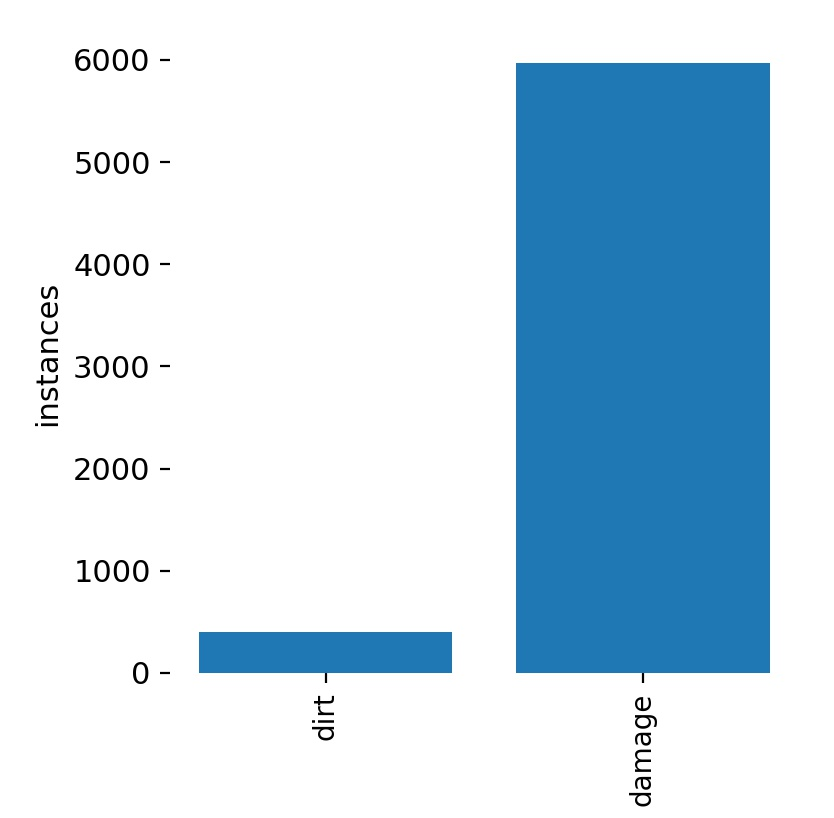
\includegraphics[width=7cm]{Images/Label Count.png}
    \caption{Instances per class}
    \label{fig:damageex}
\end{figure}


The dataset used in training and validation is one built upon the "DTU-Drone inspection images of the wind turbine"\cite{DTU}, these high resolution image were split into 586x371 pixel images and those images without any wind turbine surface within them were removed, those with negligible amounts of turbine surface were retained. Two classes were decided for labelling, those being dirt and damage: dirt composed of a large area with a high density of small dark marking on the surface of the blade, this most commonly occurred on the edge of the blade, see fig. \ref{fig:dirtex}.; damage on the other hand was a highly variable class of all other larger or isolated markings, these ranged from scratches to chipped surface material, see fig. \ref{fig:damageex}., this class has potential for further division. The labelling was done by hand using a free online tool makesense.ai \cite{make-sense}, this provided all the required functions for labelling and exported the labels directly into YOLO format. A simple Python script was made to convert these labels into COCO JSON format.

\begin{figure}[H]
    \centering
    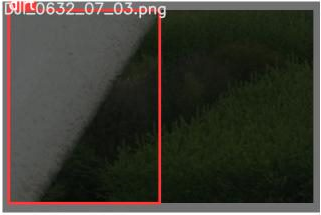
\includegraphics[width=7cm]{Images/Dirt Example.png}
    \caption{Instance of Dirt Class}
    \label{fig:dirtex}
\end{figure}


\begin{figure}[H]
    \centering
    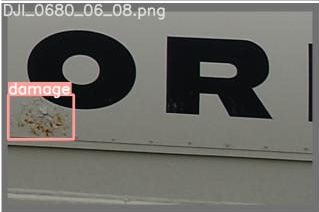
\includegraphics[width=7cm]{Images/Damage Example.png}
    \caption{Instance of Damage Class}
    \label{fig:damageex}
\end{figure}

\subsection{Data Augmentation}
Data Augmentation is automatically handled by both libraries used.

\subsection{ResNet-101 Faster R-CNN}
A Faster R-CNN Architecture with a ResNet-101 classifier was used for this work. The ResNet-101 classifier was composed of 101-layers with 33 3-layered residual blocks as described by He et al. \cite{he2015deep} the details of these layers can be seen in Table \ref{tab:R101}. The Faster R-CNN was implemented with the Detectron2 library \cite{wu2019detectron2} which allows for ease of implementation of a number of state of the art architectures built upon Pytorch. The initial weights were those pretrained on the ImageNet dataset \cite{deng2009imagenet} as provided by Detectron2. 

\begin{table}[H]
\begin{center}
\begin{tabular}{ |c|c|c| }
\hline
 layer name & output size & layer details \\ 
 \hline
 conv1 & 112x112 & 7x7, 64, stride 2 \\  
 \hline
 conv2\_x & 56x56 & $\begin{bmatrix}1\times1, 64\\3\times3, 64\\1\times1, 256\end{bmatrix}\times3$\\
 \hline
  conv3\_x & 28x28 & $\begin{bmatrix}1\times1, 128\\3\times3, 128\\1\times1, 512\end{bmatrix}\times4$\\
 \hline
  conv4\_x & 14x14 & $\begin{bmatrix}1\times1, 256\\3\times3, 256\\1\times1, 1024\end{bmatrix}\times23$\\
 \hline
  conv5\_x & 7x7 & $\begin{bmatrix}1\times1, 512\\3\times3, 512\\1\times1, 2048\end{bmatrix}\times3$\\
 \hline
  & 1x1 & average pool, 1000-d fc, softmax\\
 \hline
\end{tabular}
\vspace*{3mm}
\caption{\label{tab:R101}ResNet 101-C4 Model \cite{he2015deep}
.}
\end{center}
\end{table}


\subsection{YOLOV5}
Three models from the YOLOv5 Model family were implemented, trained and validated in this paper, that being the S or small, M or medium and L or large models. These models were implemented with the official YOLOv5 library built on Pytorch, which provided weights for each model pretrained on the COCO dataset \cite{lin2015microsoft}. A diagram of the structure of the YOLOv5L's Network prior to post processing layers is detailed in Fig. \ref{fig:yol}.

\begin{figure}[H]
    \centering
    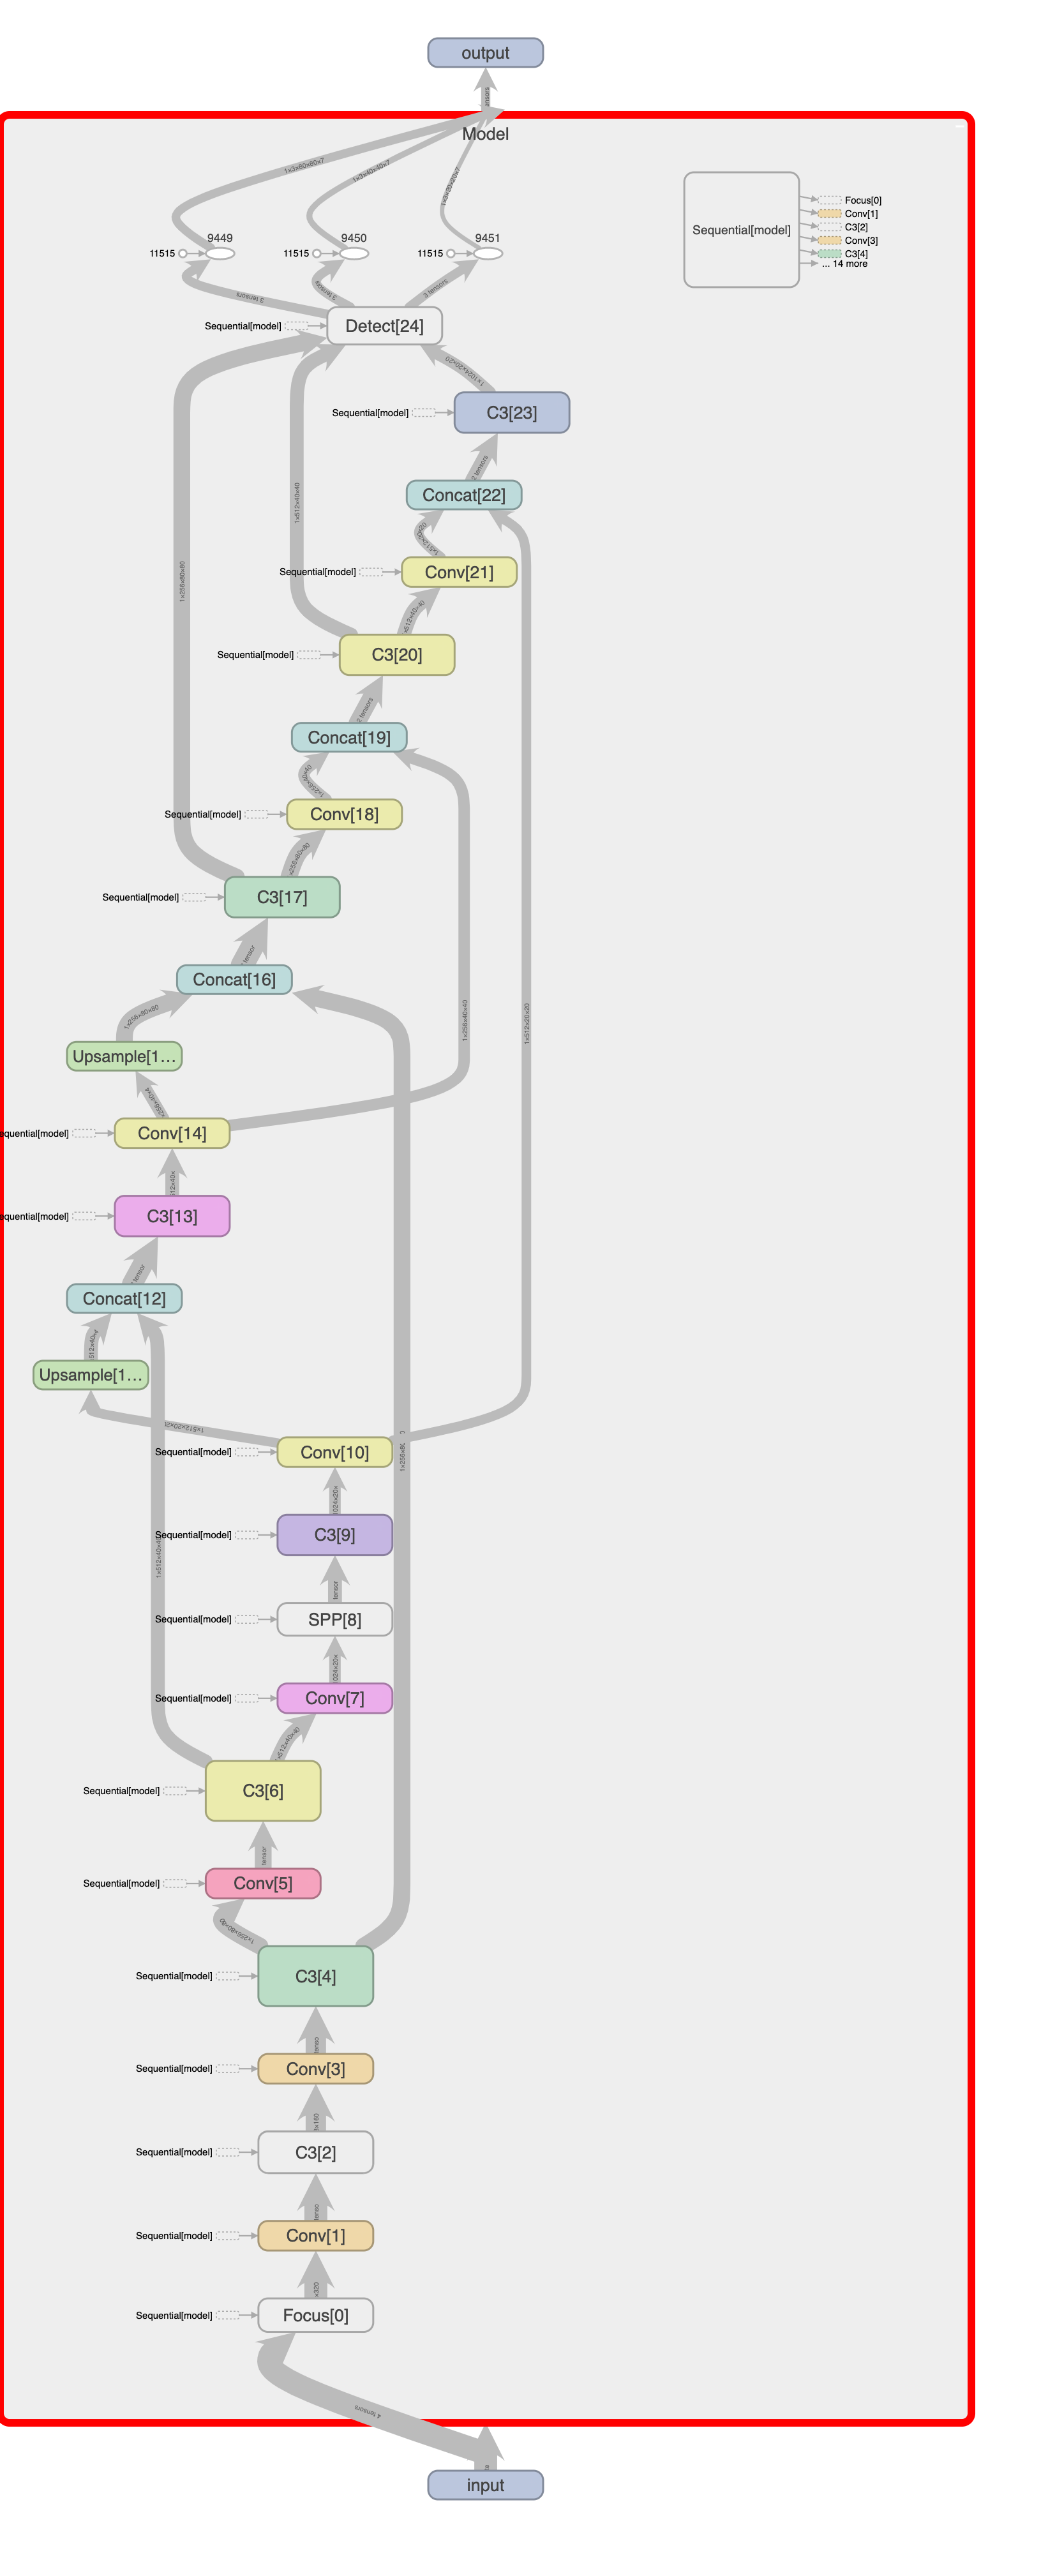
\includegraphics[width=9cm]{Images/YOLOV5L.png}
    \caption{YOLOv5L Structure Diagram}
    \label{fig:yol}
\end{figure}


\subsection{Transfer Learning}
In an effort to overcome the limited size of the dataset, transfer learning was implemented through another surface defect dataset, that being the NEU-DET dataset \cite{he_song_meng_yan_2019}, all the networks were trained to learn to detect the given steel surface defects, in the belief that prior training would towards the identification of features such as scratches on steel surfaces, could in turn be applicable in the identification of scratches on the surfaces of wind turbines.

\subsection{Training}
Training was performed on a machine running a Windows Operating system fitted with an Nvidea GTX 1080 Ti Graphics with 11 GB of VRAM. For the YOLOv5 models, training consisted of 1000 epochs with a batch size of 16, this duration was chosen as it allowed the convergence of the loss calculated on the validation set, the batch size was chosen to give the greatest VRAM usage possible on the YOLOv5L.

\begin{figure}[H]
    \centering
    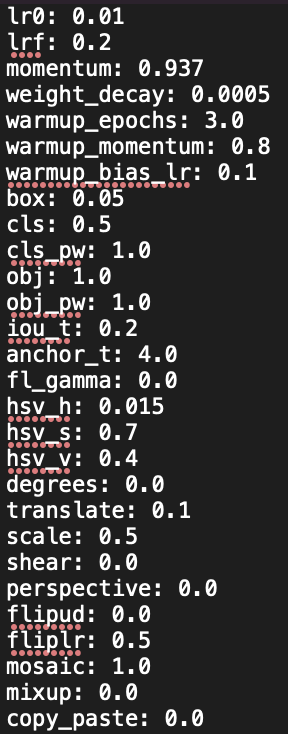
\includegraphics[width=3cm]{Images/YoloHyperparameters.png}
    \caption{YOLOv5 Hyper-parameter values}
    \label{fig:hyp}
\end{figure}

The Faster R-CNN was run for 100,000 epochs. A trial and error approach was used for finding the ideal training hyper parameters and options, this resulted in a batch size of 128, 4 images per batch and a base learning rate of .0025.

 
\section{Results}

The final mAP values for the approaches are detailed in Table \ref{tab:Map} as can be seen all the YOLO Architectures outperformed the Faster R-CNN Architecture across both mAP@0.5 and mAP@0.5:0.95. The method with the highest mAP values was YOLOv5s.

\begin{table}[H]
\begin{center}
\begin{tabular}{ |c|c|c| }
\hline
  & mAP@.5:.95 & mAP@0.5  \\ 
 \hline
 Faster R-CNN ResNet-101-C4 & 0.4743 & 0.7539 \\  
 \hline
 YOLOv5s & 0.5121 & 0.7937 \\
 \hline
 YOLOv5m & 0.4989 & 0.7837 \\
 \hline
 YOLOv5L & 0.4931 & 0.7836 \\
 \hline
\end{tabular}
\vspace*{3mm}
\caption{\label{tab:Map}mAP Values
.}
\end{center}
\end{table}
 
 Fig. \ref{fig:YoloMapValues} Provides the graph of change in mAP values over the training process, as can be seen the YOLOv5s' mAP values increase at the greatest rate, and YOLOv5L at lowest rate. The mAP@0.5:0.95 values generally seem to increase through out the training process, whereas the mAP@0.5 reaches a apex and subsequently decreases. The highest mAP@0.5 value is given by YOLOv5m halfway through the 1000 epochs, while the highest mAP@0.5:0.95 is provided by YOLOv5s towards the final epochs.
  
\begin{figure}[H]
    \centering
    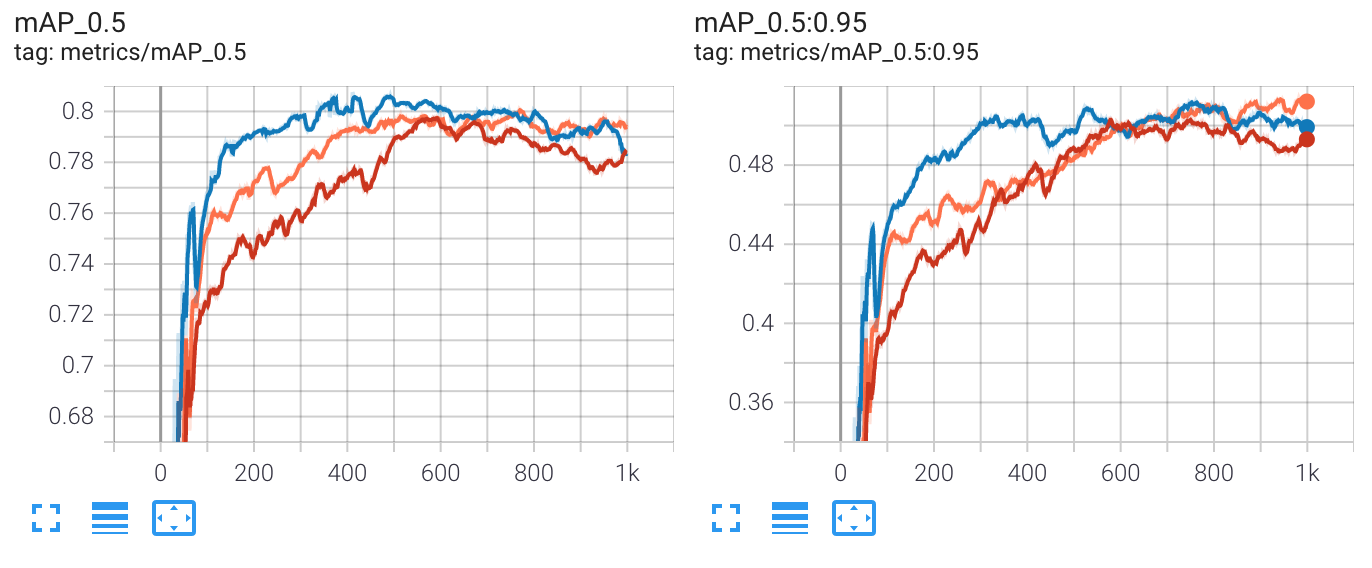
\includegraphics[width=8cm]{Images/yolomaps.png}
    \caption{YOLOv5 mAP Values with YOLOv5s in Yellow, YOLOv5m in blue, and YOLOv5L in Red}
    \label{fig:YoloMapValues}
\end{figure}

Fig. \ref{fig:yolopr} is a graph of the Precision and Recall of the YOLO models over the course of training. The YOLOv5m has the greatest precision value however this value drops towards the end of training and YOLOv5s has the greatest final precision value. The greatest recall value is provided by YOLOv5L as 0.82.

\begin{figure}[H]
\centering
\begin{subfigure}{.2\textwidth}
    \centering
    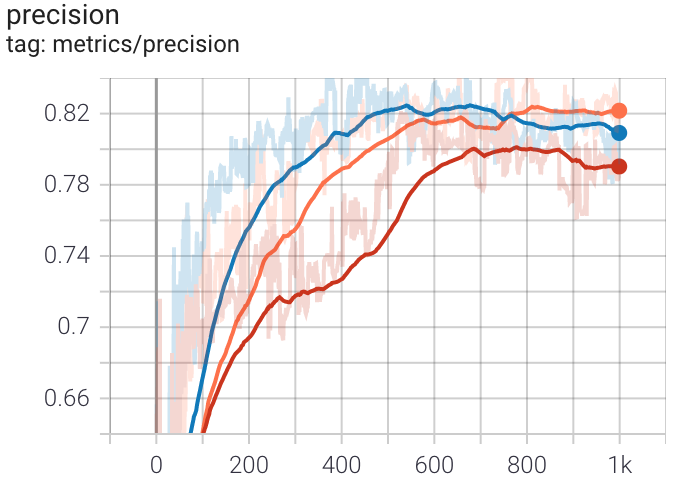
\includegraphics[width=1\linewidth]{Images/Precission.png}
\end{subfigure}%
\begin{subfigure}{.2\textwidth}
    \centering
    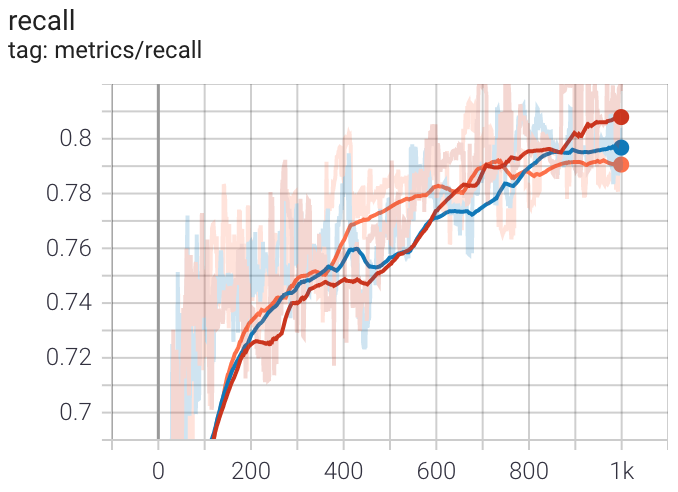
\includegraphics[width=1\linewidth]{Images/Recall.png}
\end{subfigure}
\caption{YOLO Precision and Recall Graphs}
\label{fig:yolopr}
\end{figure}

Fig. \ref{fig:FasterRCNNmAP} shows a graph of the mAP values for the Faster R-CNN ResNet-101-C4 method, as seen in the the graphs for YOLOv5 the mAP@0.5 increases to an apex and then decreases after that, the mAP@0.5:0.95 however steadily increases up to the final epoch.


\begin{figure}[H]
\centering
\begin{subfigure}{.2\textwidth}
    \centering
    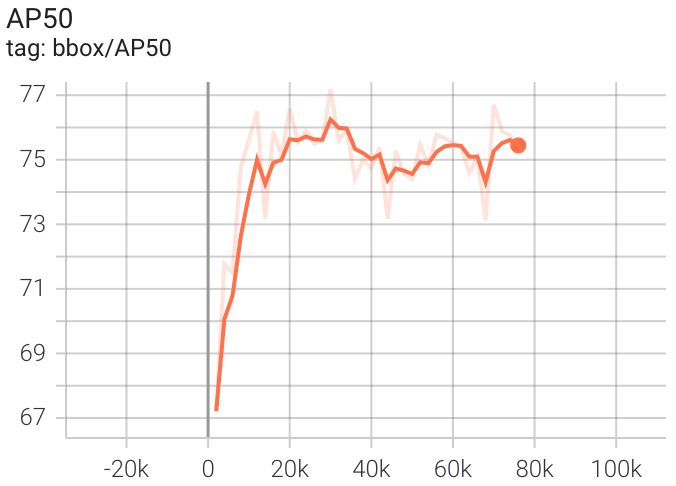
\includegraphics[width=1\linewidth]{Images/Faster/AP50.png}
    \caption{mAP@0.5}
\end{subfigure}%
\begin{subfigure}{.2\textwidth}
    \centering
    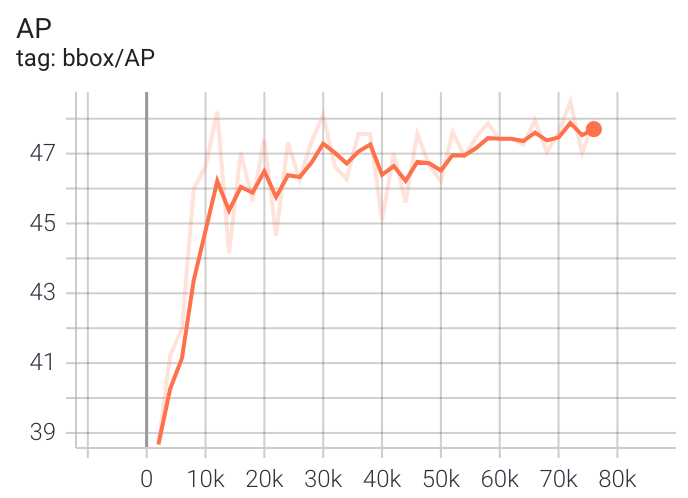
\includegraphics[width=1\linewidth]{Images/Faster/AP.png}
    \caption{mAP@0.5:0.95} 
\end{subfigure}
\caption{Faster R-CNN ResNet-101-C4 mAP graphs}
\label{fig:FasterRCNNmAP}
\end{figure}

Fig. \ref{fig:DensePreds} show a predictions for both faster R-CNN and YOLOv5s on an image containing densly packed bouding boxes, these can be compared to Fig. 
\ref{fig:DenseTruth}. which show the true bounding boxes, this comparison shows Faster R-CNN matches more closely the Truth than YOLOv5s in this scenario.
\begin{figure}[H]
\centering
\begin{subfigure}{.2\textwidth}
    \centering
    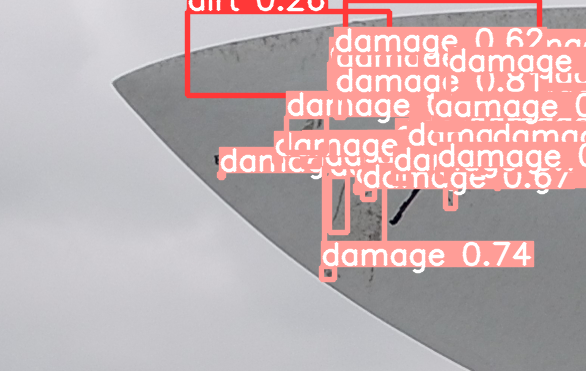
\includegraphics[width=1\linewidth]{Images/YOLOPrediction.png}
    \caption{YOLOv5s}
\end{subfigure}%
\begin{subfigure}{.2\textwidth}
    \centering
    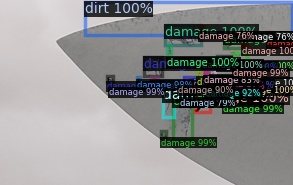
\includegraphics[width=1\linewidth]{Images/FasterPrediction.jpg}
    \caption{Faster R-CNN} 
\end{subfigure}
\caption{Predictions on a highly instance dense image}
\label{fig:DensePreds}
\end{figure}

\begin{figure}[H]
    \centering
    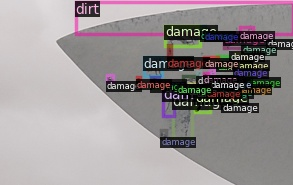
\includegraphics[width=4cm]{Images/True.jpg}
    \caption{True Bounding Boxes for highly instance dense image}
    \label{fig:DenseTruth}
\end{figure}

Beyond the Object detection on static images, the trained models was used to perform object detection on a Youtube video of Drone footage \cite{OriginalVid}, one for YOLOv5s \cite{YOLOv5svid} and one for Faster R-CNN \cite{FasterRCNNvid}. The inference speeds for each model is given in Fig. \ref{tab:infspeed}

\begin{table}[H]
\begin{center}
\begin{tabular}{ |c|c|c|c|c| }
\hline
  & YOLOv5s & YOLOv5m & YOLOv5L & Faster R-CNN  \\ 
 \hline
 Speed & 17.6 FPS & 12.2 FPS & 8.5 FPS & 1.7 FPS  \\
  \hline
\end{tabular}
\vspace*{3mm}
\caption{\label{tab:infspeed}Inference Speed of Methods
.}
\end{center}
\end{table}

\section{Discussion}
Based on the results, it seems that some of the Models were under-trained, however the mAP values of the YOLOv5s reaching over 0.80 in places is still a respectable performance for the problem. Fig. \ref{fig:YoloMapValues} show YOLOv5L being outperformed by YOLOv5s \& YOLOv5m, this unexpected result seems mostly likely to be a result of under-training, and it is predicted that if the number of epochs was doubled the YOLOv5L would start to outperform the other two models. Evidence for this is suggested in Fig. \ref{fig:yolopr} In which the recall value seems to increasing further for this model, and as recall values are component values of the AP value that form mAP, it is safe to suggest that, as long as precision isn't too negatively effected, further improvement of recall would lead to a greater mAP value. The Faster R-CNN method seems as though it could also benefit from a longer training period, this is suggested as, even though mAP@0.5 is stable, mAP@0.5:0.95 seems to be increasing further. The YOLOv5 families performance advantage as compared to the Faster R-CNN method was to be expected, however the true extent to this performance advantage is hard to quantify with the possible under-fitting problem, it should not be too hard to improve upon the performances described here. 

The Object detection performed on the Youtube Video footage proved some interesting results, the YOLOv5s provided the fastest inference speed at 17.6 FPS, this was to be expected based on descriptions of the method. All the YOLO methods outperformed the Faster R-CNN method significantly, one again this is to be expected as the YOLO architecture was designed in such a way as to minimise inference time through the single neural network \cite{redmon2016you}. An interesting note in the performance of the two methods in the produced Youtube videos is the difference in the bounding boxes used when identifying the same object tended to follow a similar pattern, the Faster RCNN approach tended to identify an entire instance of damage as a single prediction, YOLOv5s however tended to identify only portions of the damage, an example of this can be seen in the difference between Fig. \ref{fig:yolvid} \& Fig. \ref{fig:fasvid}. Beyond this YOLO generally seemed to perform better, and while detected a lot of false positives on the background, it was a lot less discriminate with its predictions on the blades too lending itself towards human assisted damage detection. While not a perfect implementation, damage detection was performed on a moving wind turbine, and damage on the surface of the blades was automatically detected, this proves the applicability these techniques in this scenario, such an approach could potentially speed up the damage inspection process significantly by proposing areas of potential damage to a human inspector, such as providing those frames from video footage annotated with bounding boxes.

\begin{figure}[H]
    \centering
    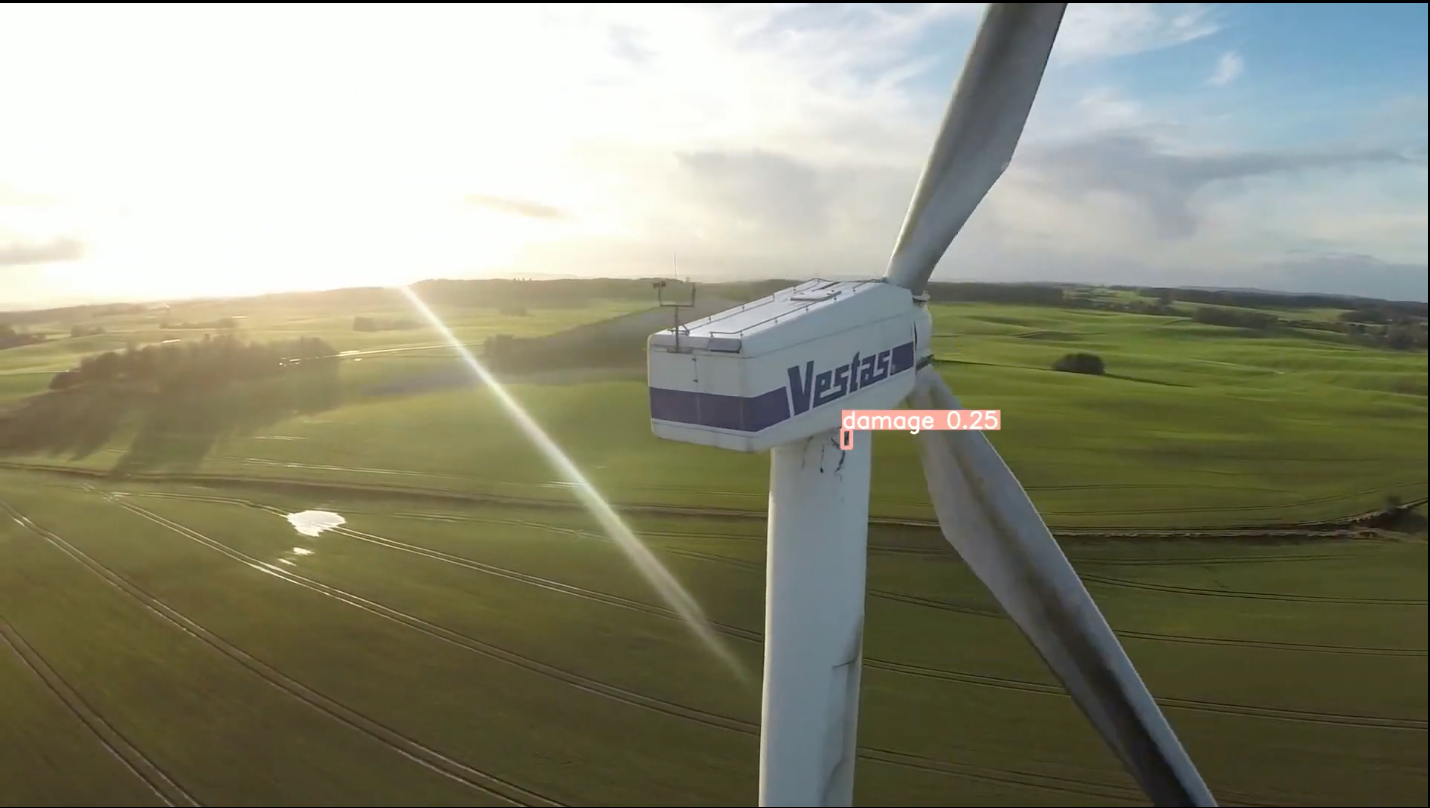
\includegraphics[width=8cm]{Images/YOLOVid.png}
    \caption{YOLOv5s Video detection}
    \label{fig:yolvid}
\end{figure}

\begin{figure}[H]
    \centering
    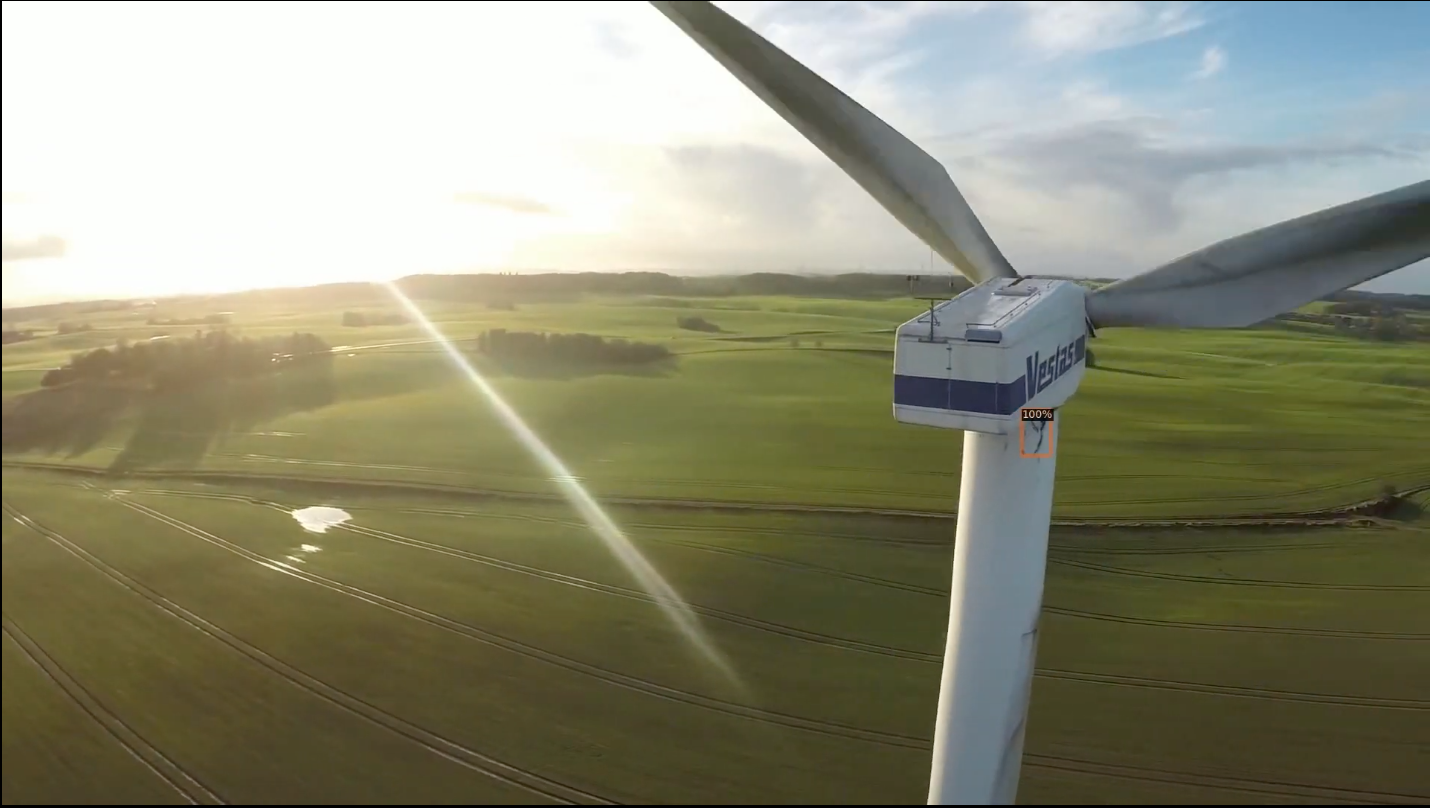
\includegraphics[width=8cm]{Images/FastVid.png}
    \caption{Faster R-CNN Video detection}
    \label{fig:fasvid}
\end{figure}

An issue that may have had a detrimental effect on the video based detection, is the lack of variety in the instances of damage in the created dataset, this may have had a significant negative effect on the models' ability to generalise about new forms of damage. The dataset has many images of the same damage repeated at different angles, and the repeated occurrence of the same forms of damage likely led to learning of features specific to those specific damage instances, rather than the general feature in common to all potential damage. This could be resolved by expanding the dataset with new images to provide a more varied set of damage instances. Another potential avenue would be the use of more classes as per Sakar et al.'s work \cite{sarkar2021wind}, this would allow an exploration of which kinds of damage are the most difficult to identify correctly

\section{Conclusion}
This Work presented a fully annotated publicly available Dataset for Wind Turbine Surface damage detection, and provides some benchmark performance values using Faster R-CNN with a ResNet-101-C4 classifer and a number of YOLOv5 implementation. This work further uses the trained models to perform object detection on drone footage of a moving drone on an active wind turbine, proving the applicability of the used technologies towards AI-assisted or fully autonomous inspections on actively running wind turbines, potentially saving significant costs due to downtime. An interesting avenue of future research is the use of segmentation techniques on video footage to provide more specific descriptions of the wind turbine damage, and the annotating of wind turbine damage for segmentation using CAM representations as described in \cite{crous2018combining}. The proposed dataset could easily be expanded given additional footage to allow for higher quality predictions and, in the authors opinion, doing so would be of considerable value. 

\bibliographystyle{abbrv}
\bibliography{bib}

\cleardoublepage
\appendix

\subsection{Annotation Stats}

\begin{figure}[H]
    \centering
    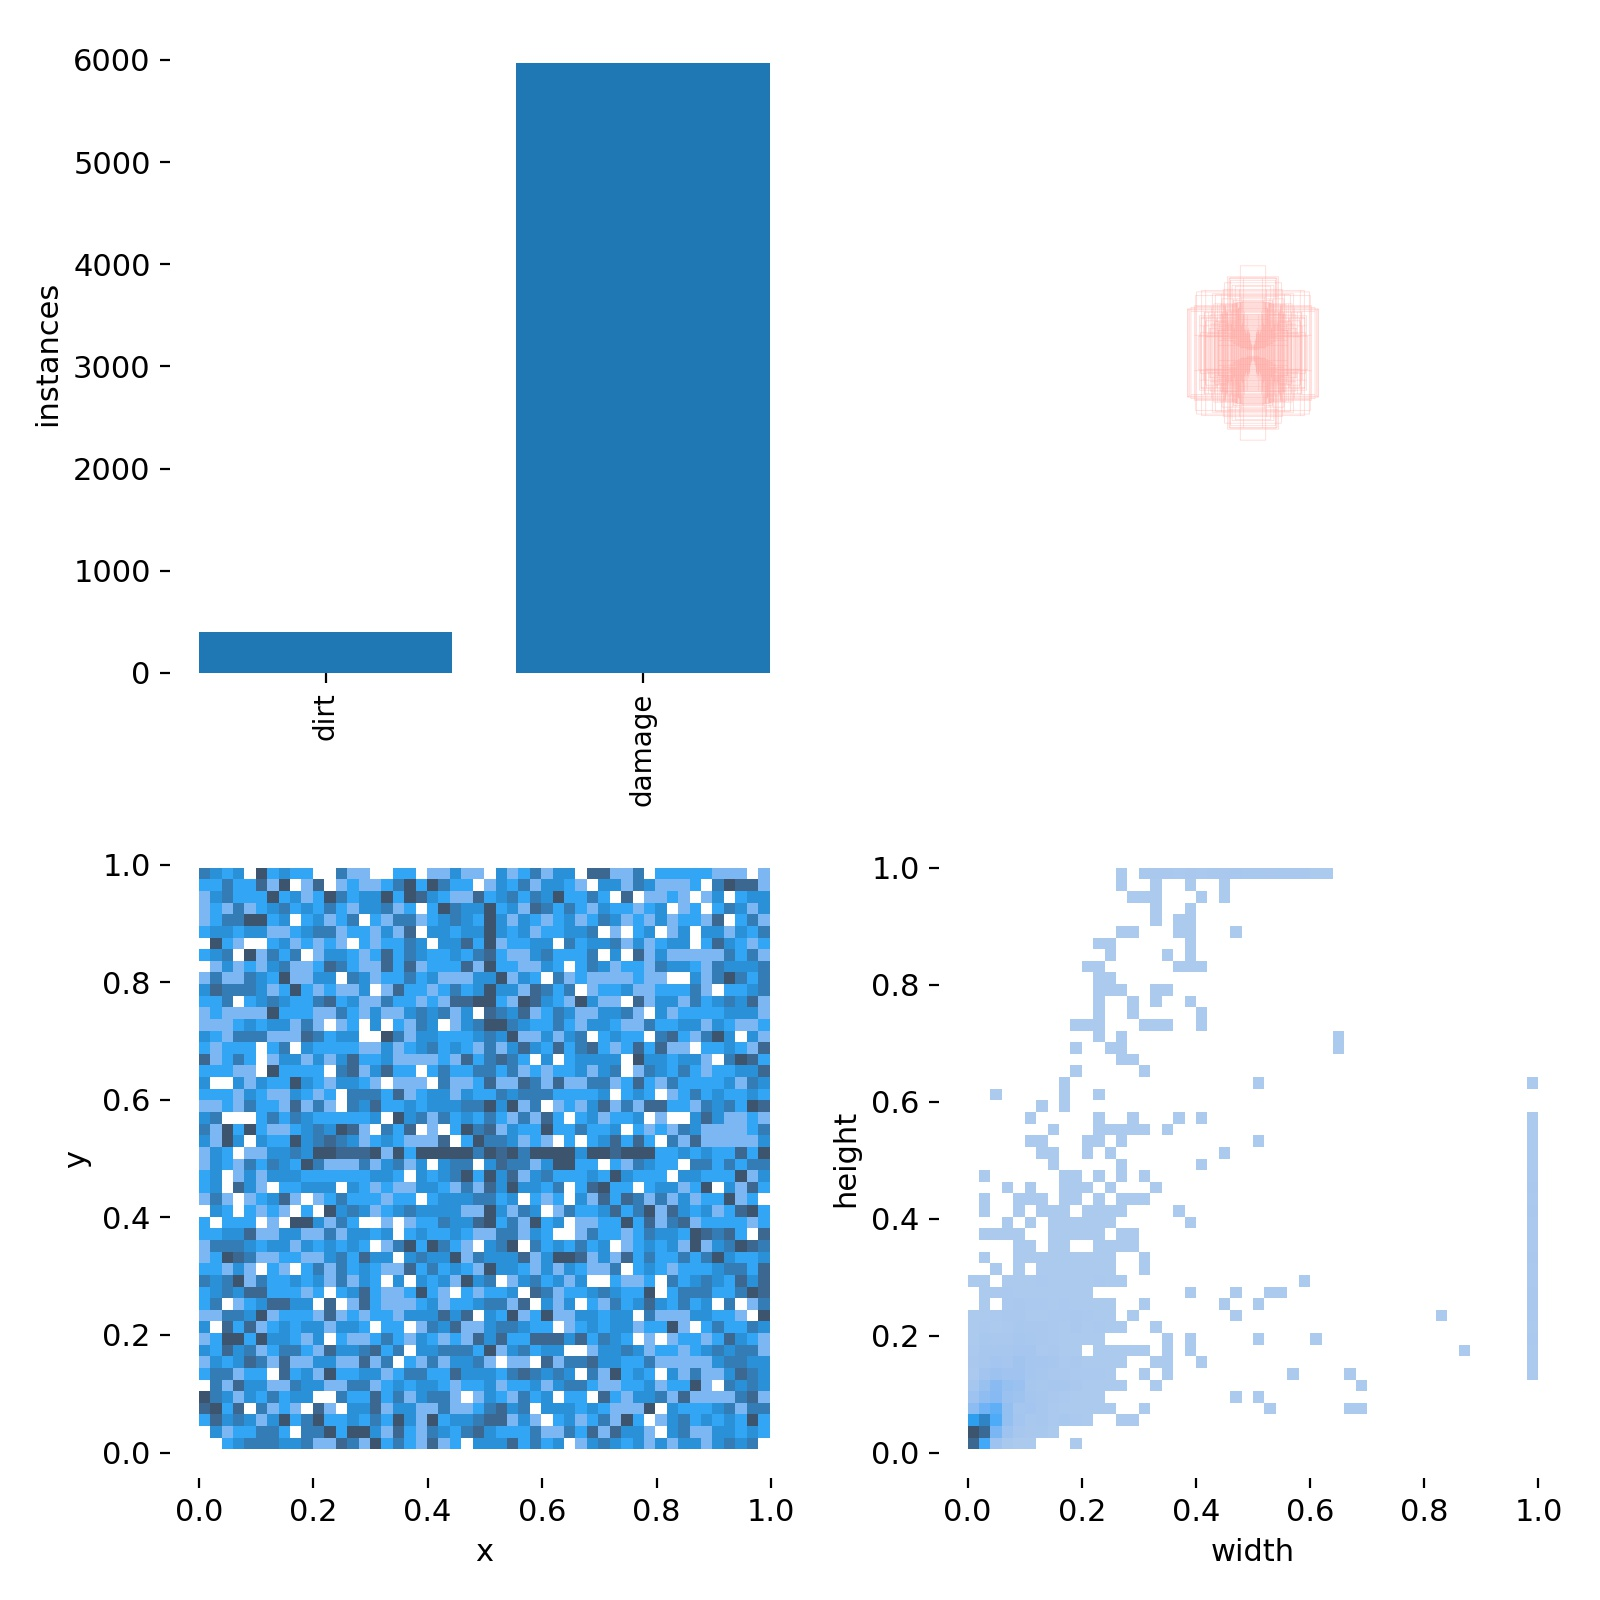
\includegraphics[width=8cm]{Images/YOLOv5L/labels.jpg}
    \caption{Label Statistics}
\end{figure}

\begin{figure}[H]
    \centering
    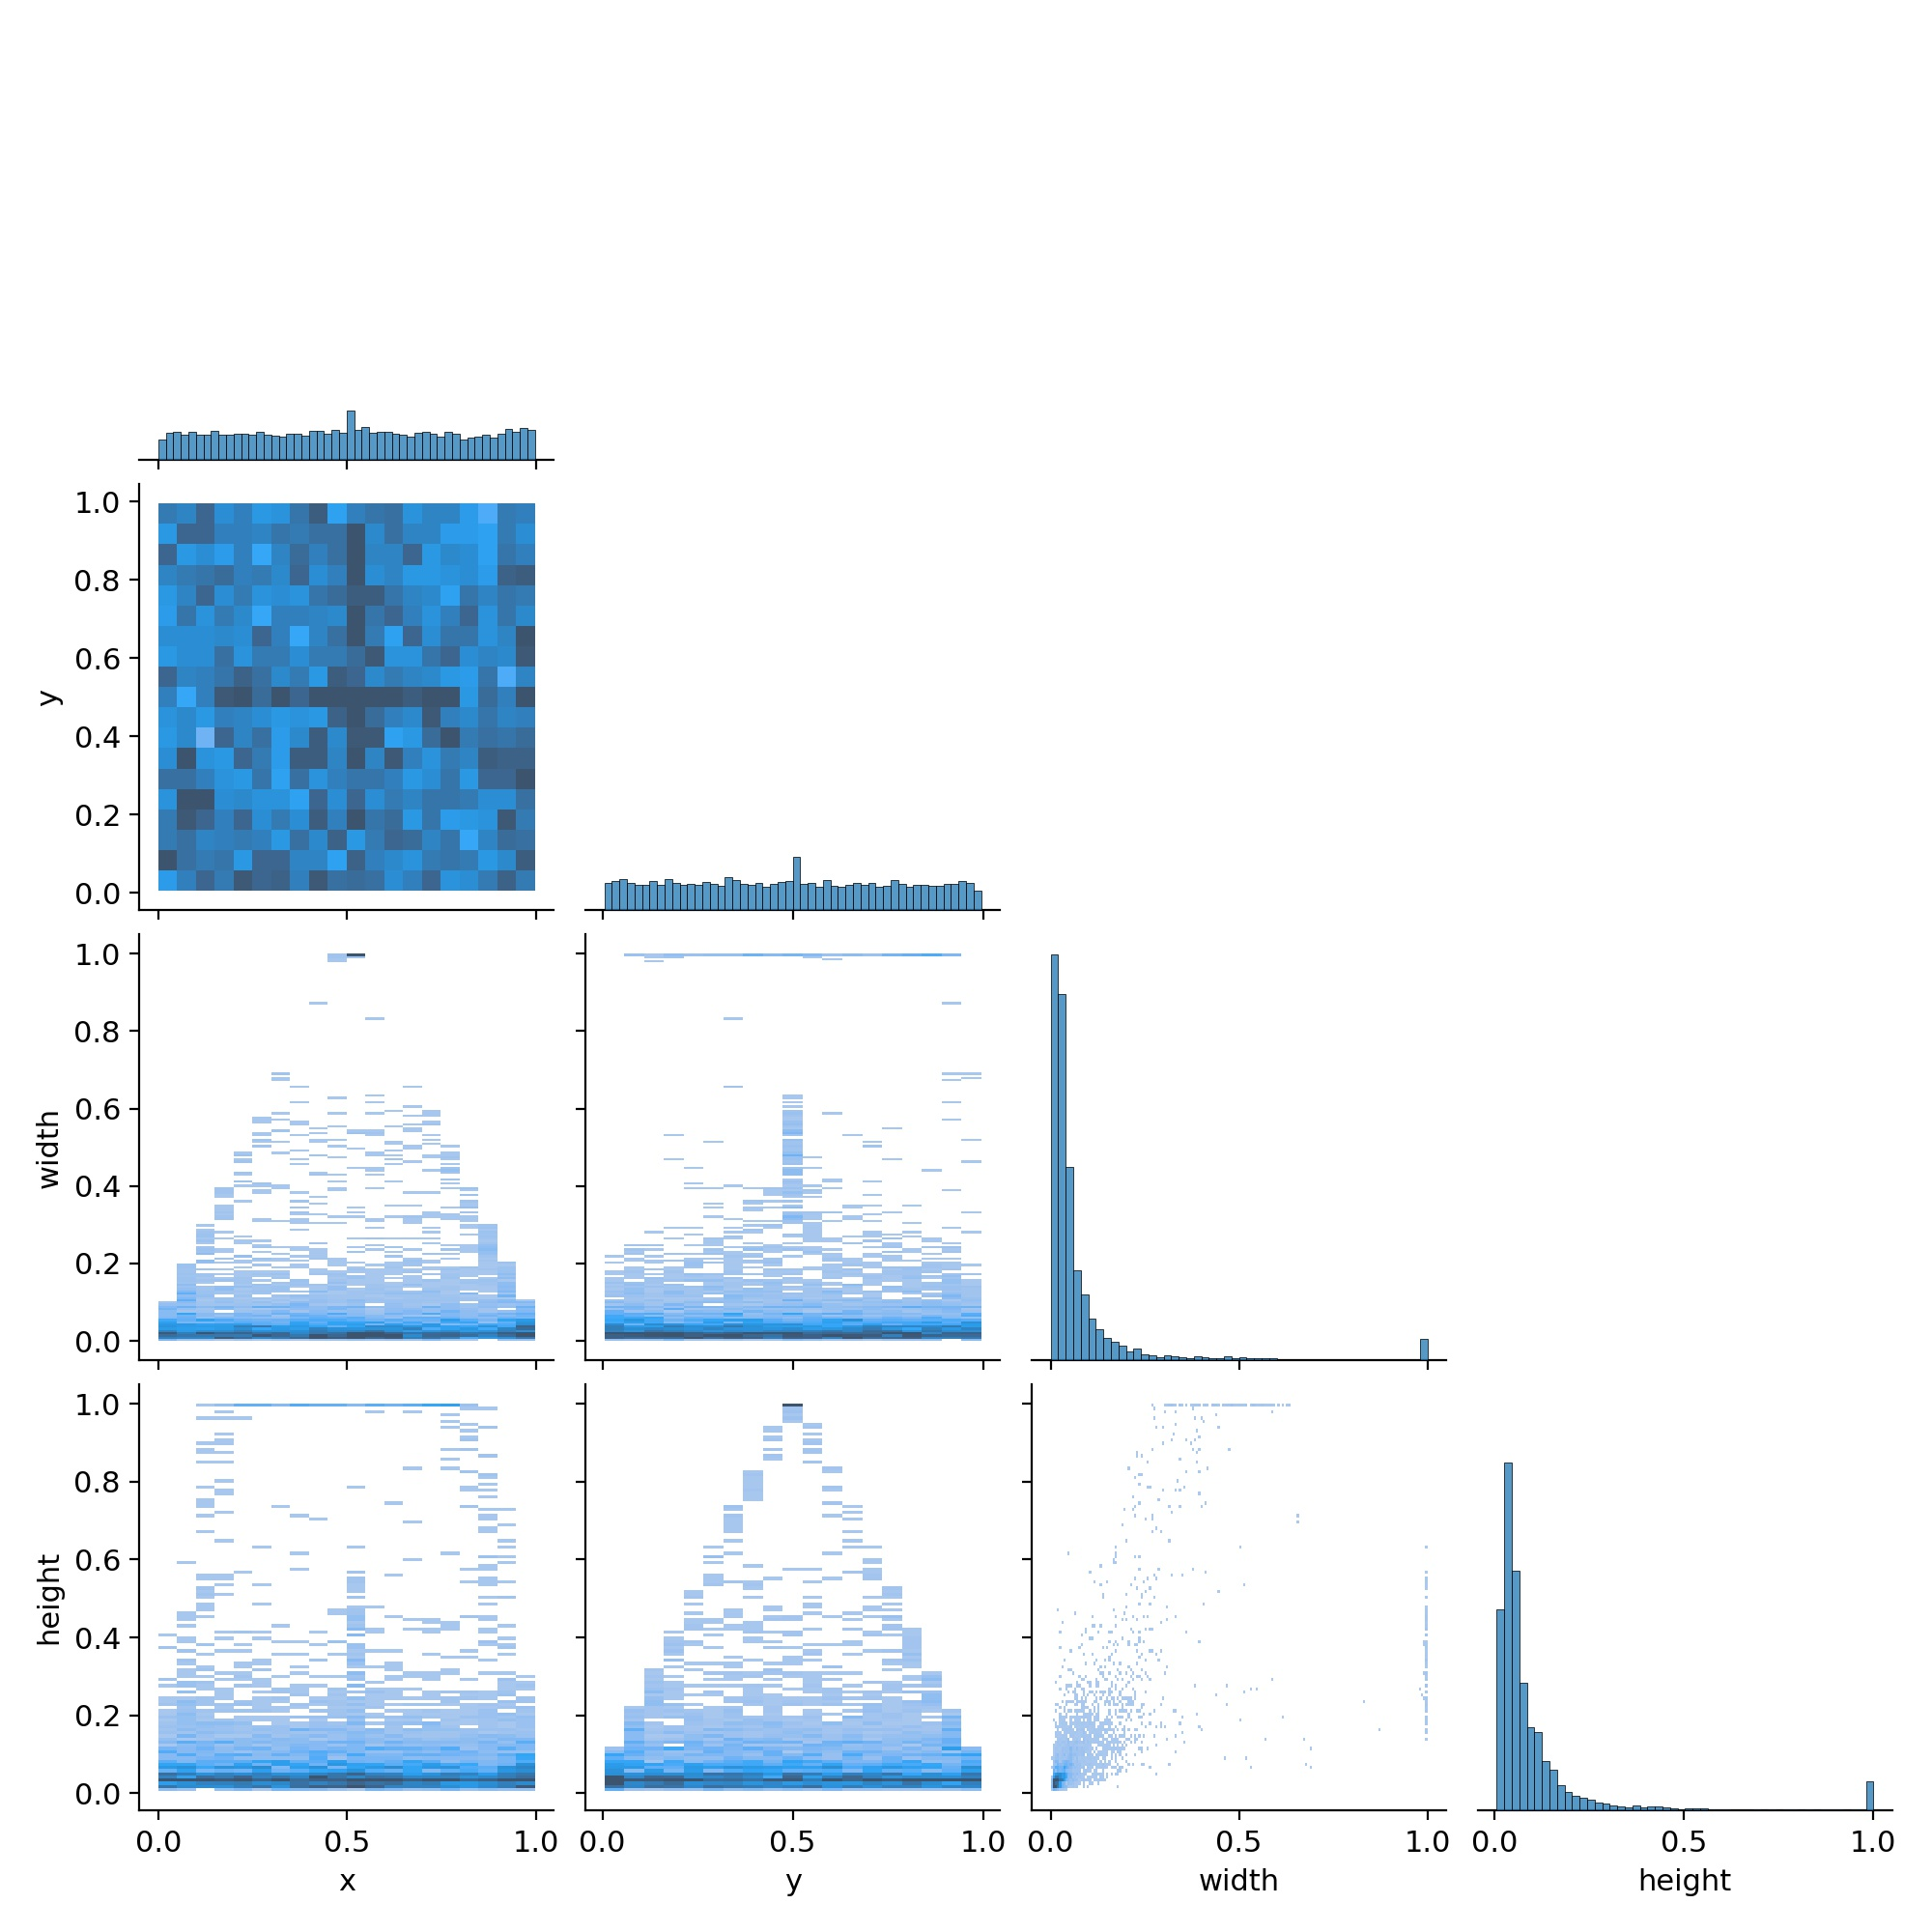
\includegraphics[width=8cm]{Images/YOLOv5L/labels_correlogram.jpg}
    \caption{Label correlogram}
\end{figure}

\cleardoublepage
\subsection{YOLOv5L}

\begin{figure}[H]
    \centering
    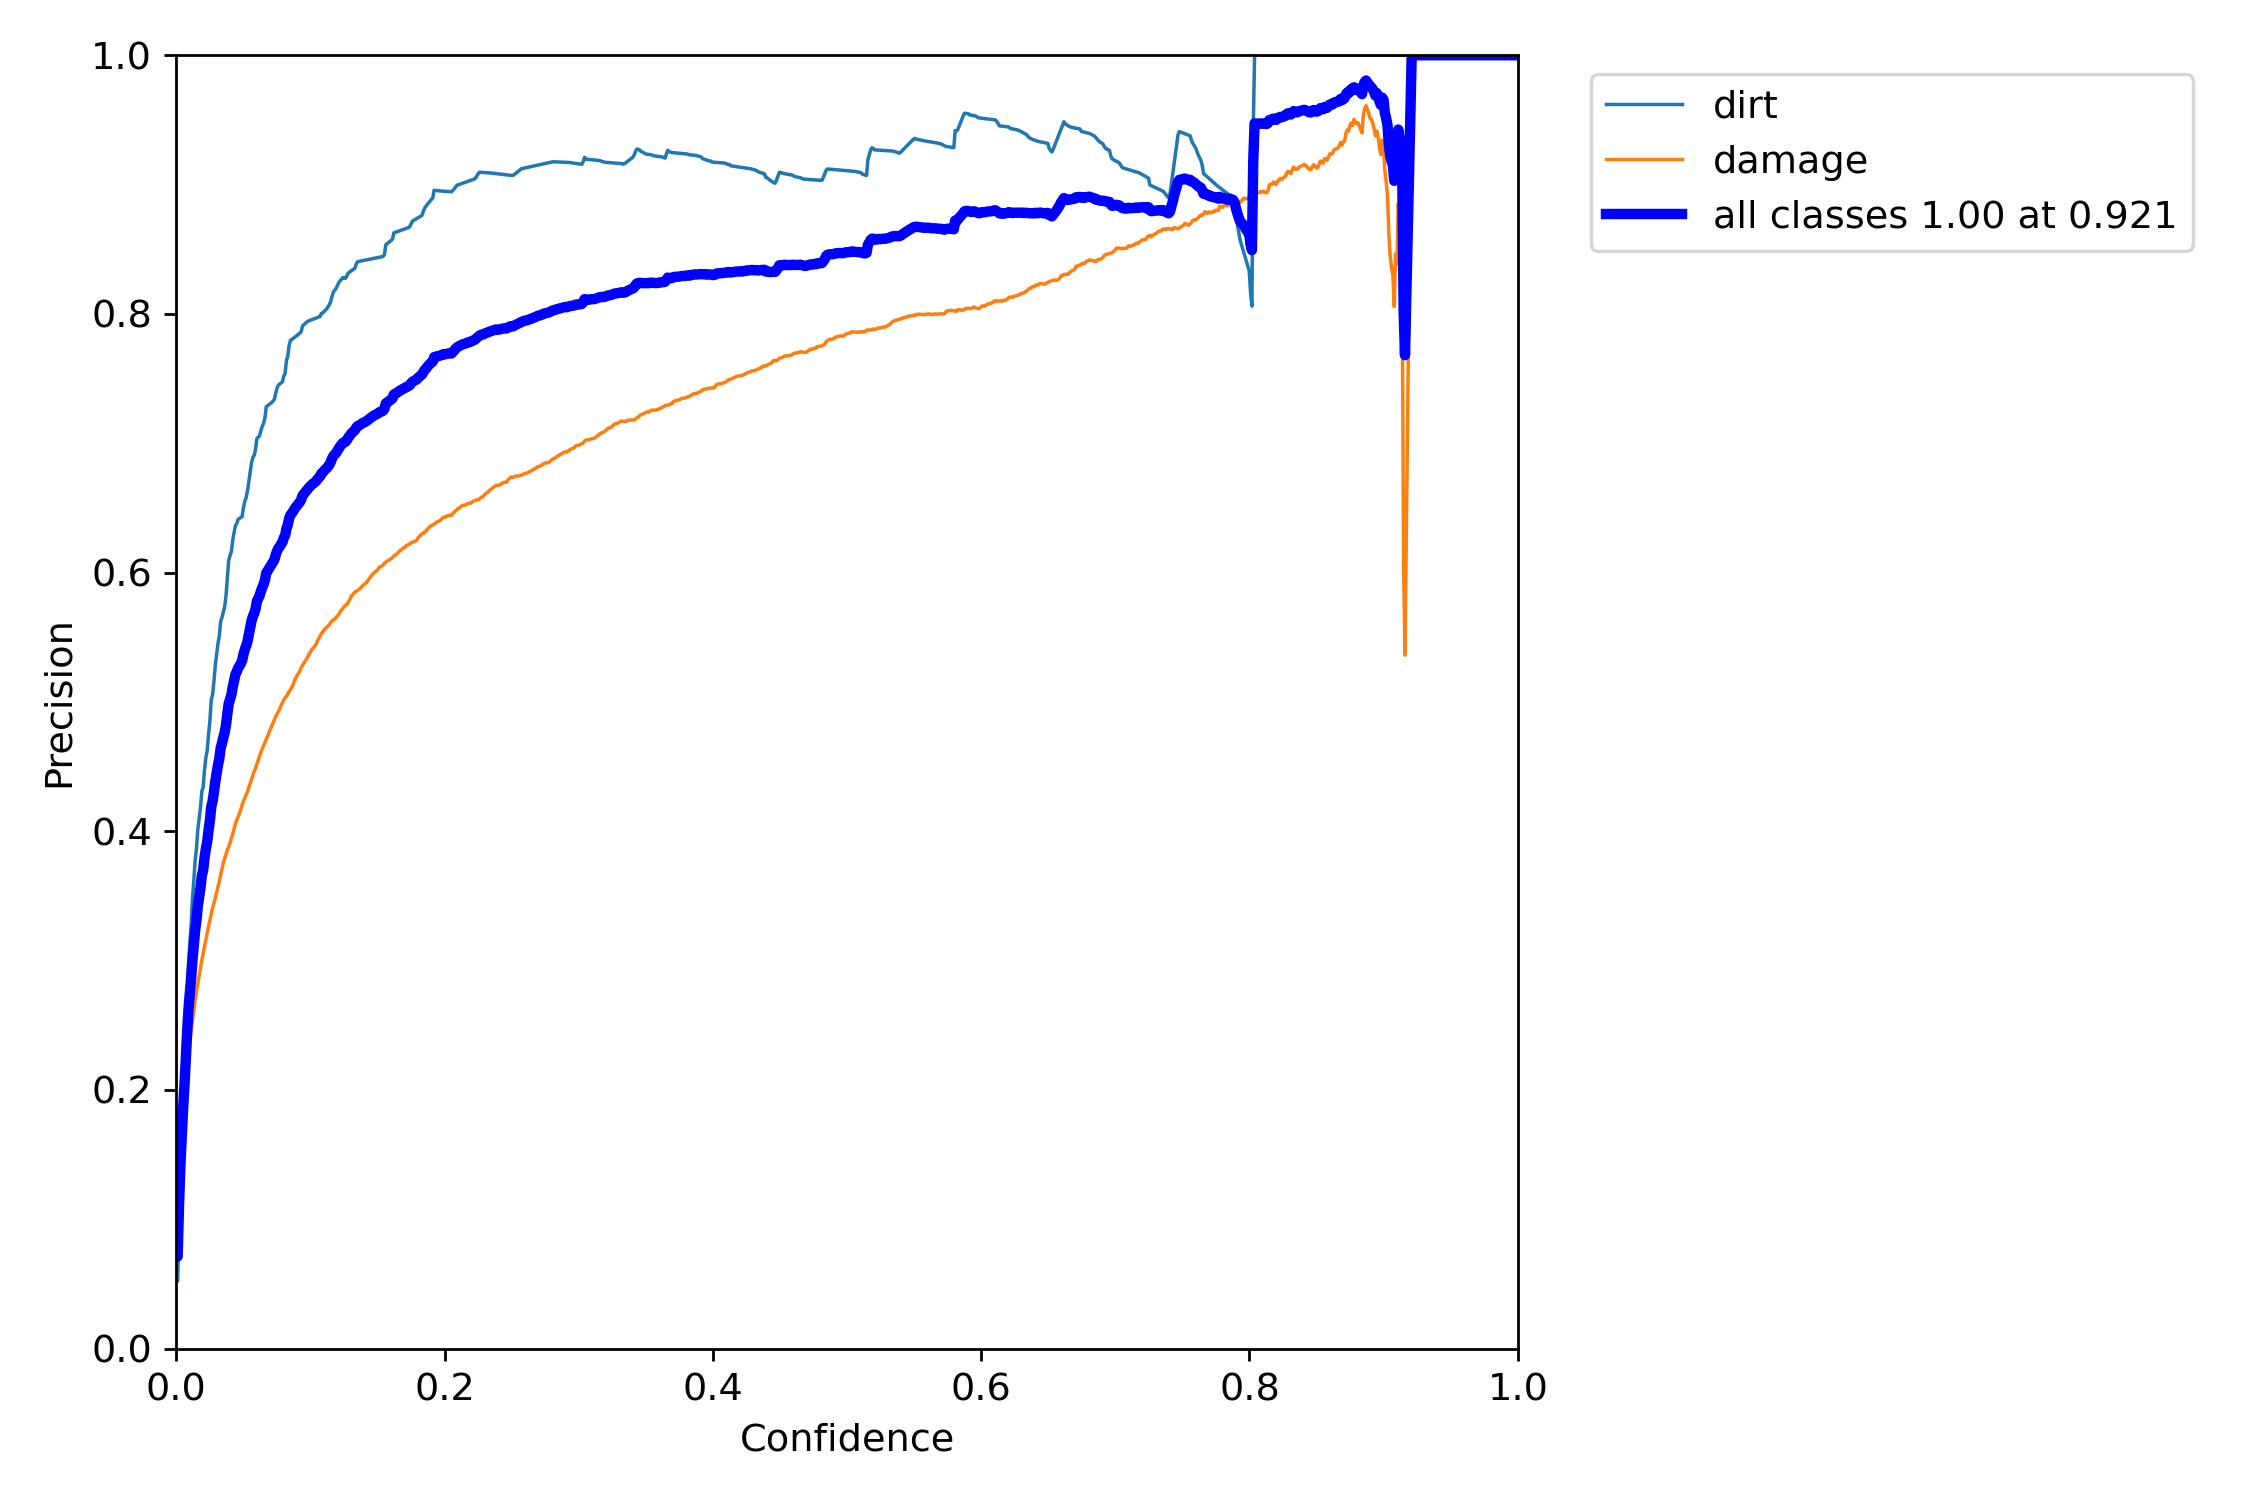
\includegraphics[width=8cm]{Images/YOLOv5L/P_curve.png}
    \caption{Precision-Curve}
\end{figure}
\begin{figure}[H]
    \centering
    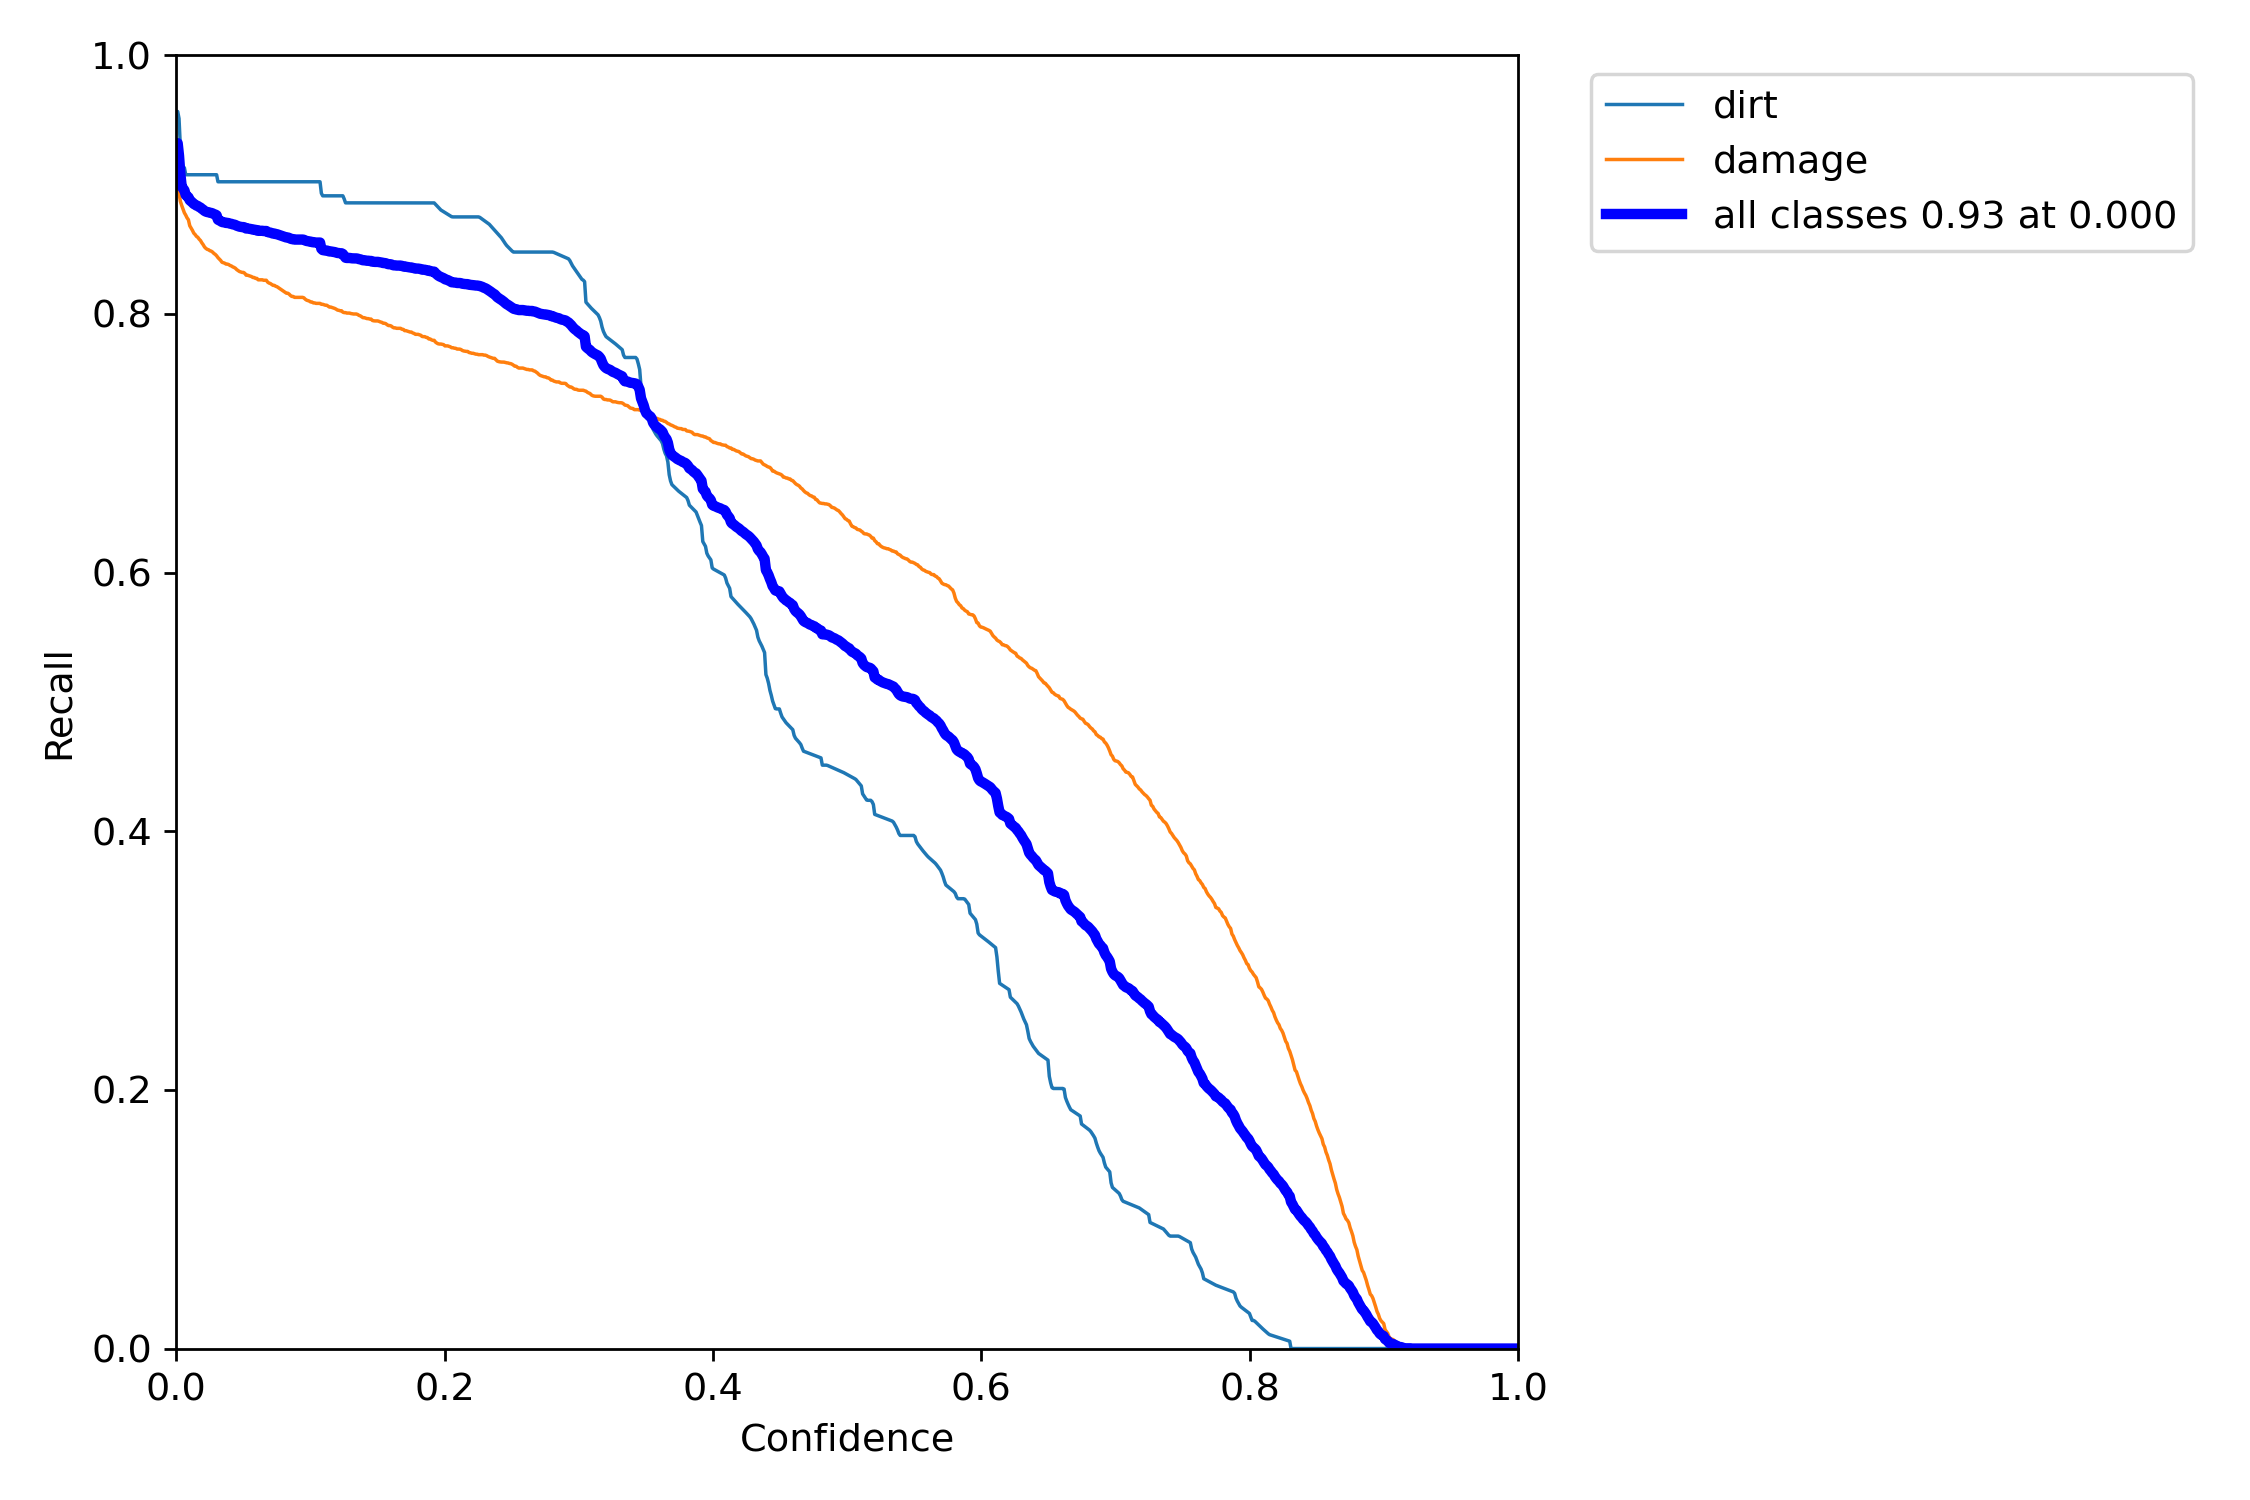
\includegraphics[width=8cm]{Images/YOLOv5L/R_curve.png}
    \caption{Recall-Curve}
\end{figure}
\begin{figure}[H]
    \centering
    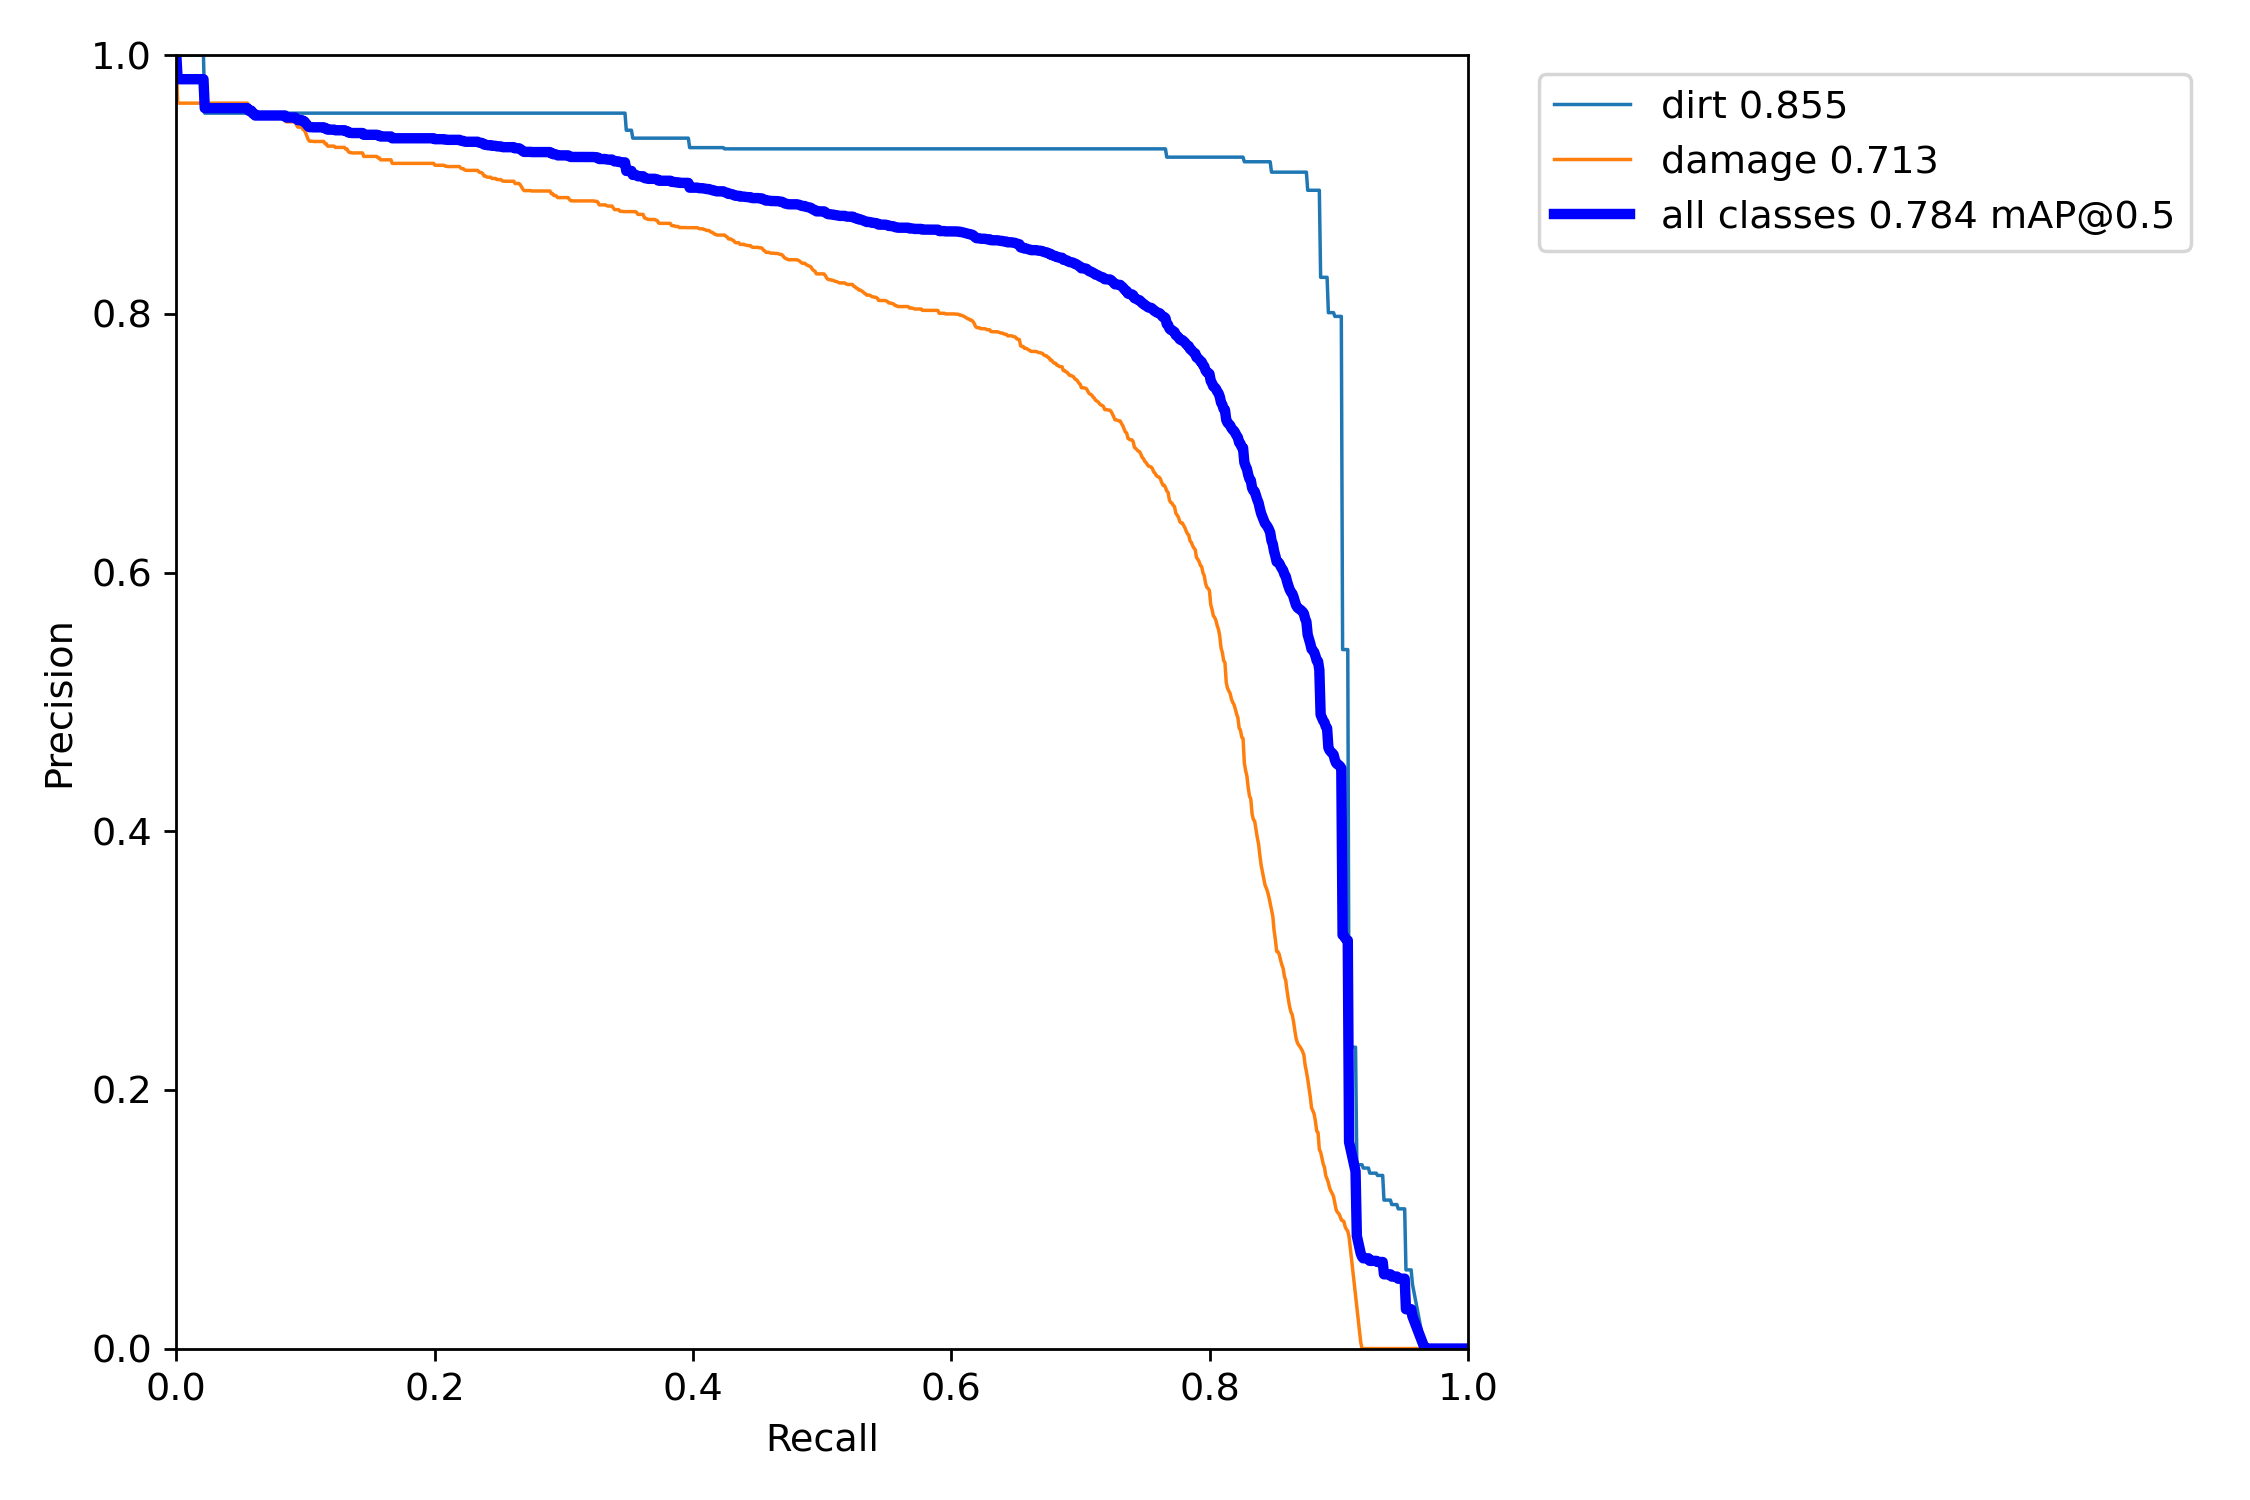
\includegraphics[width=8cm]{Images/YOLOv5L/PR_curve.png}
    \caption{PR-Curve}
\end{figure}
\begin{figure}[H]
    \centering
    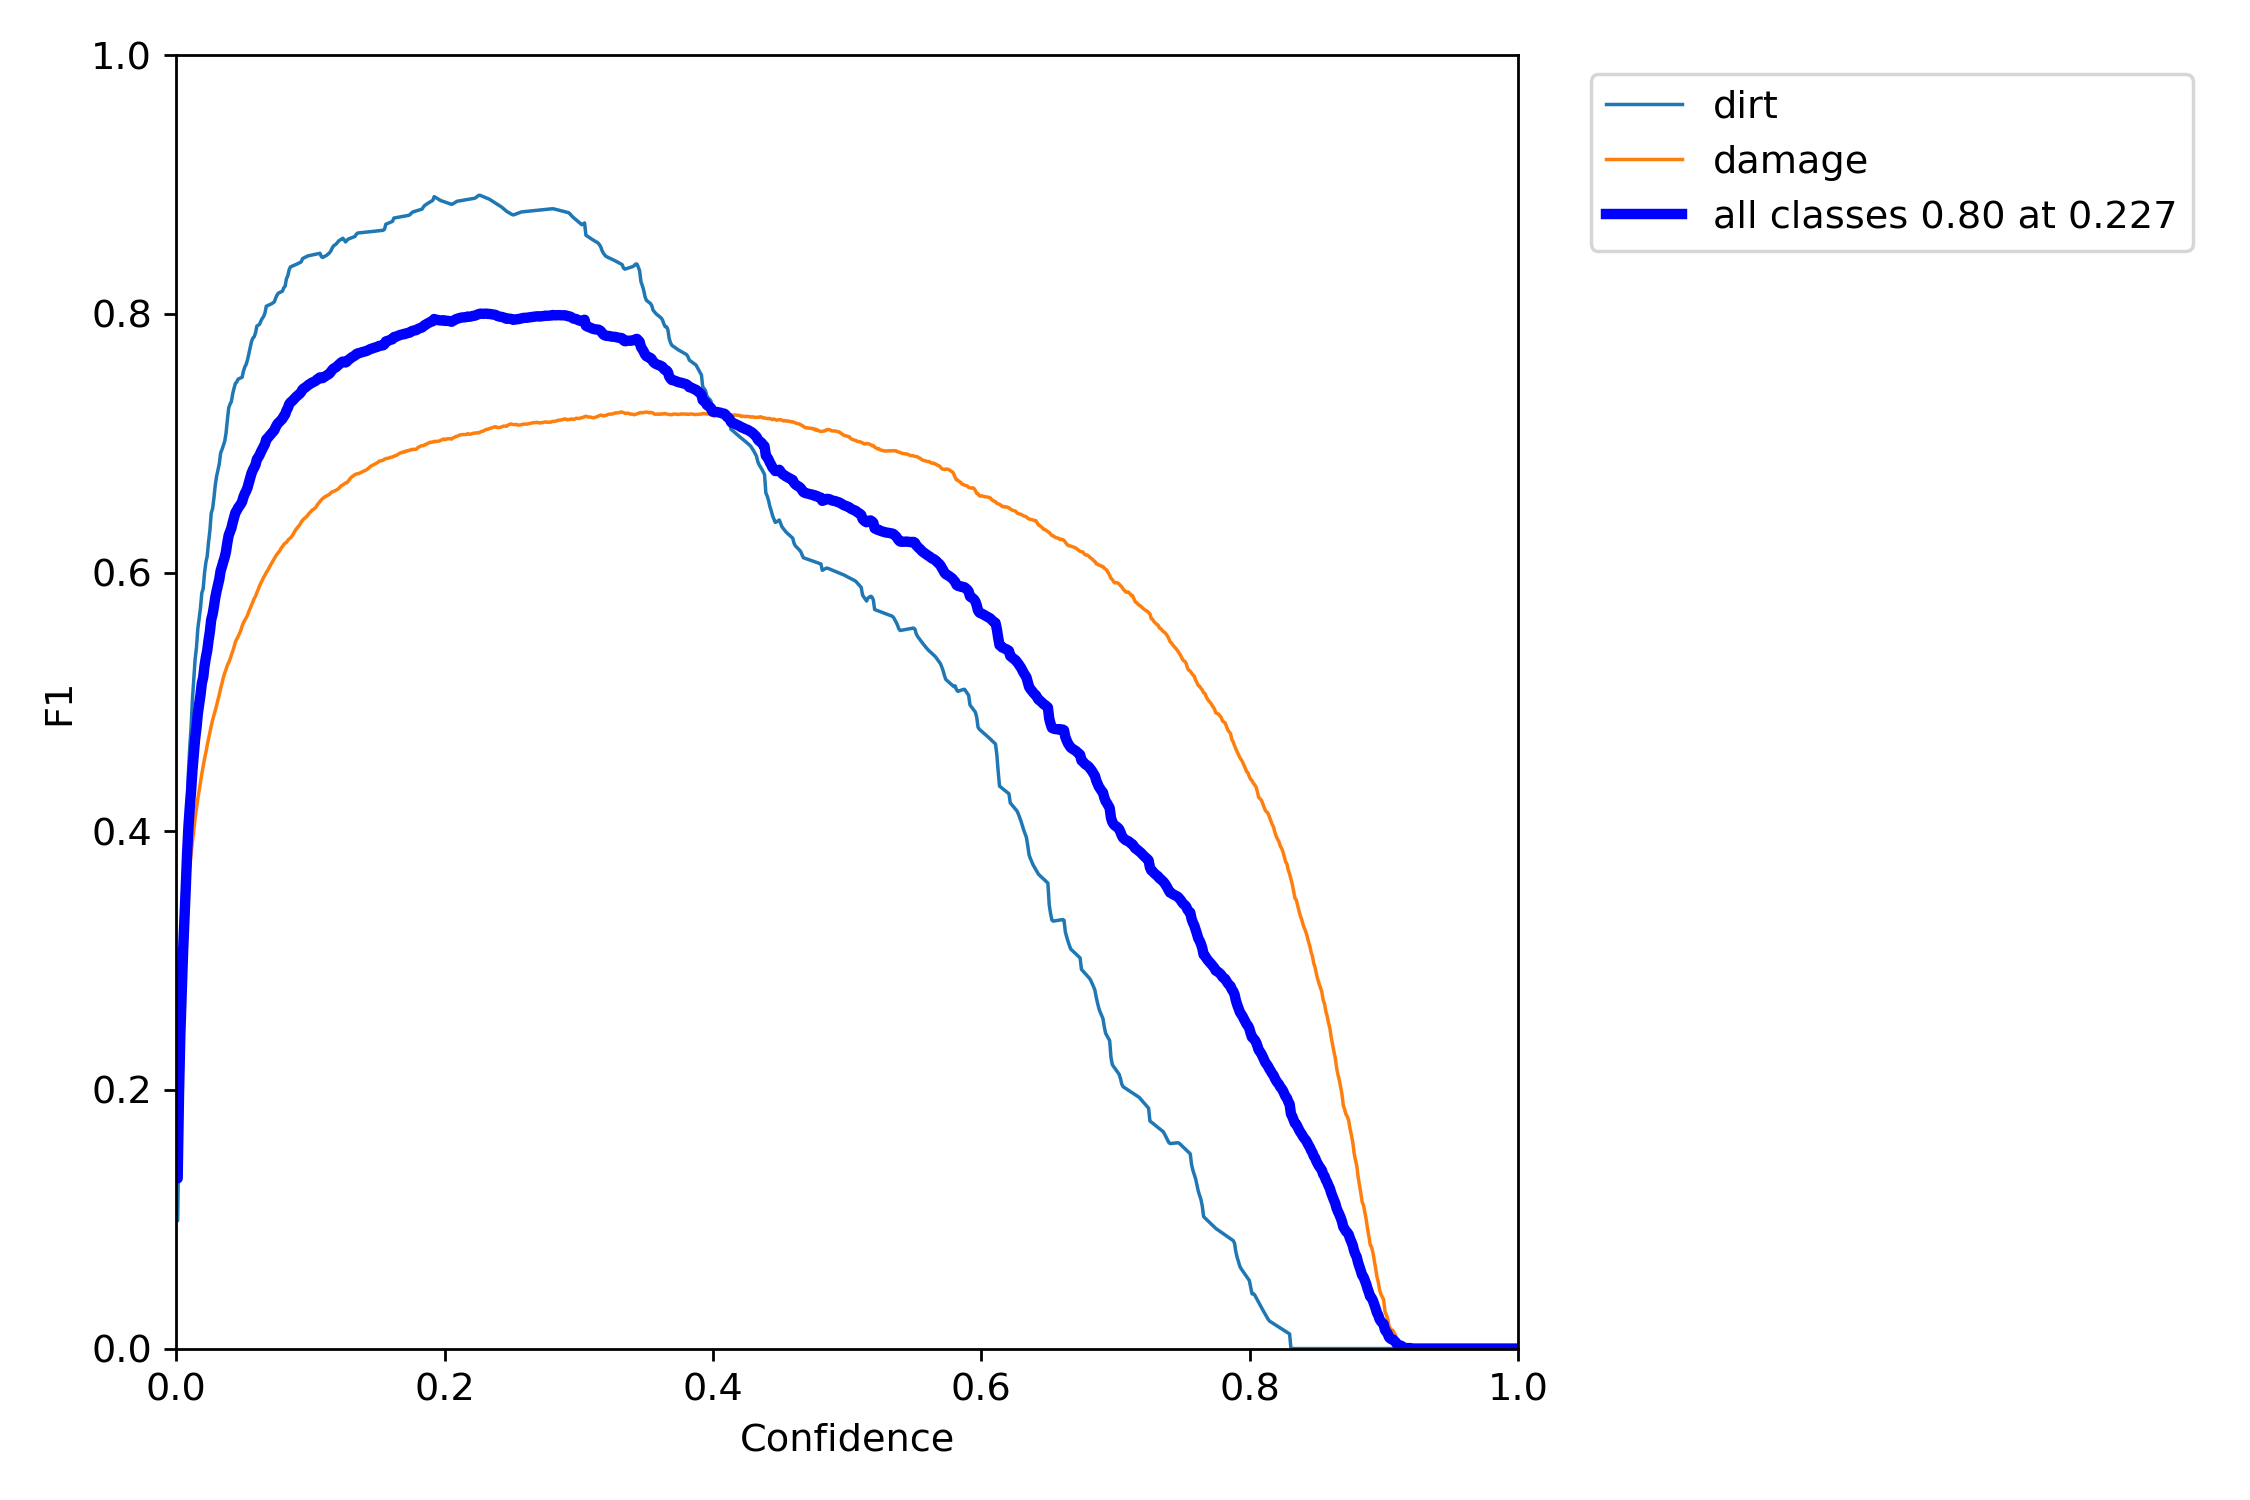
\includegraphics[width=8cm]{Images/YOLOv5L/F1_curve.png}
    \caption{F1-Curve}
\end{figure}
\begin{figure}[H]
    \centering
    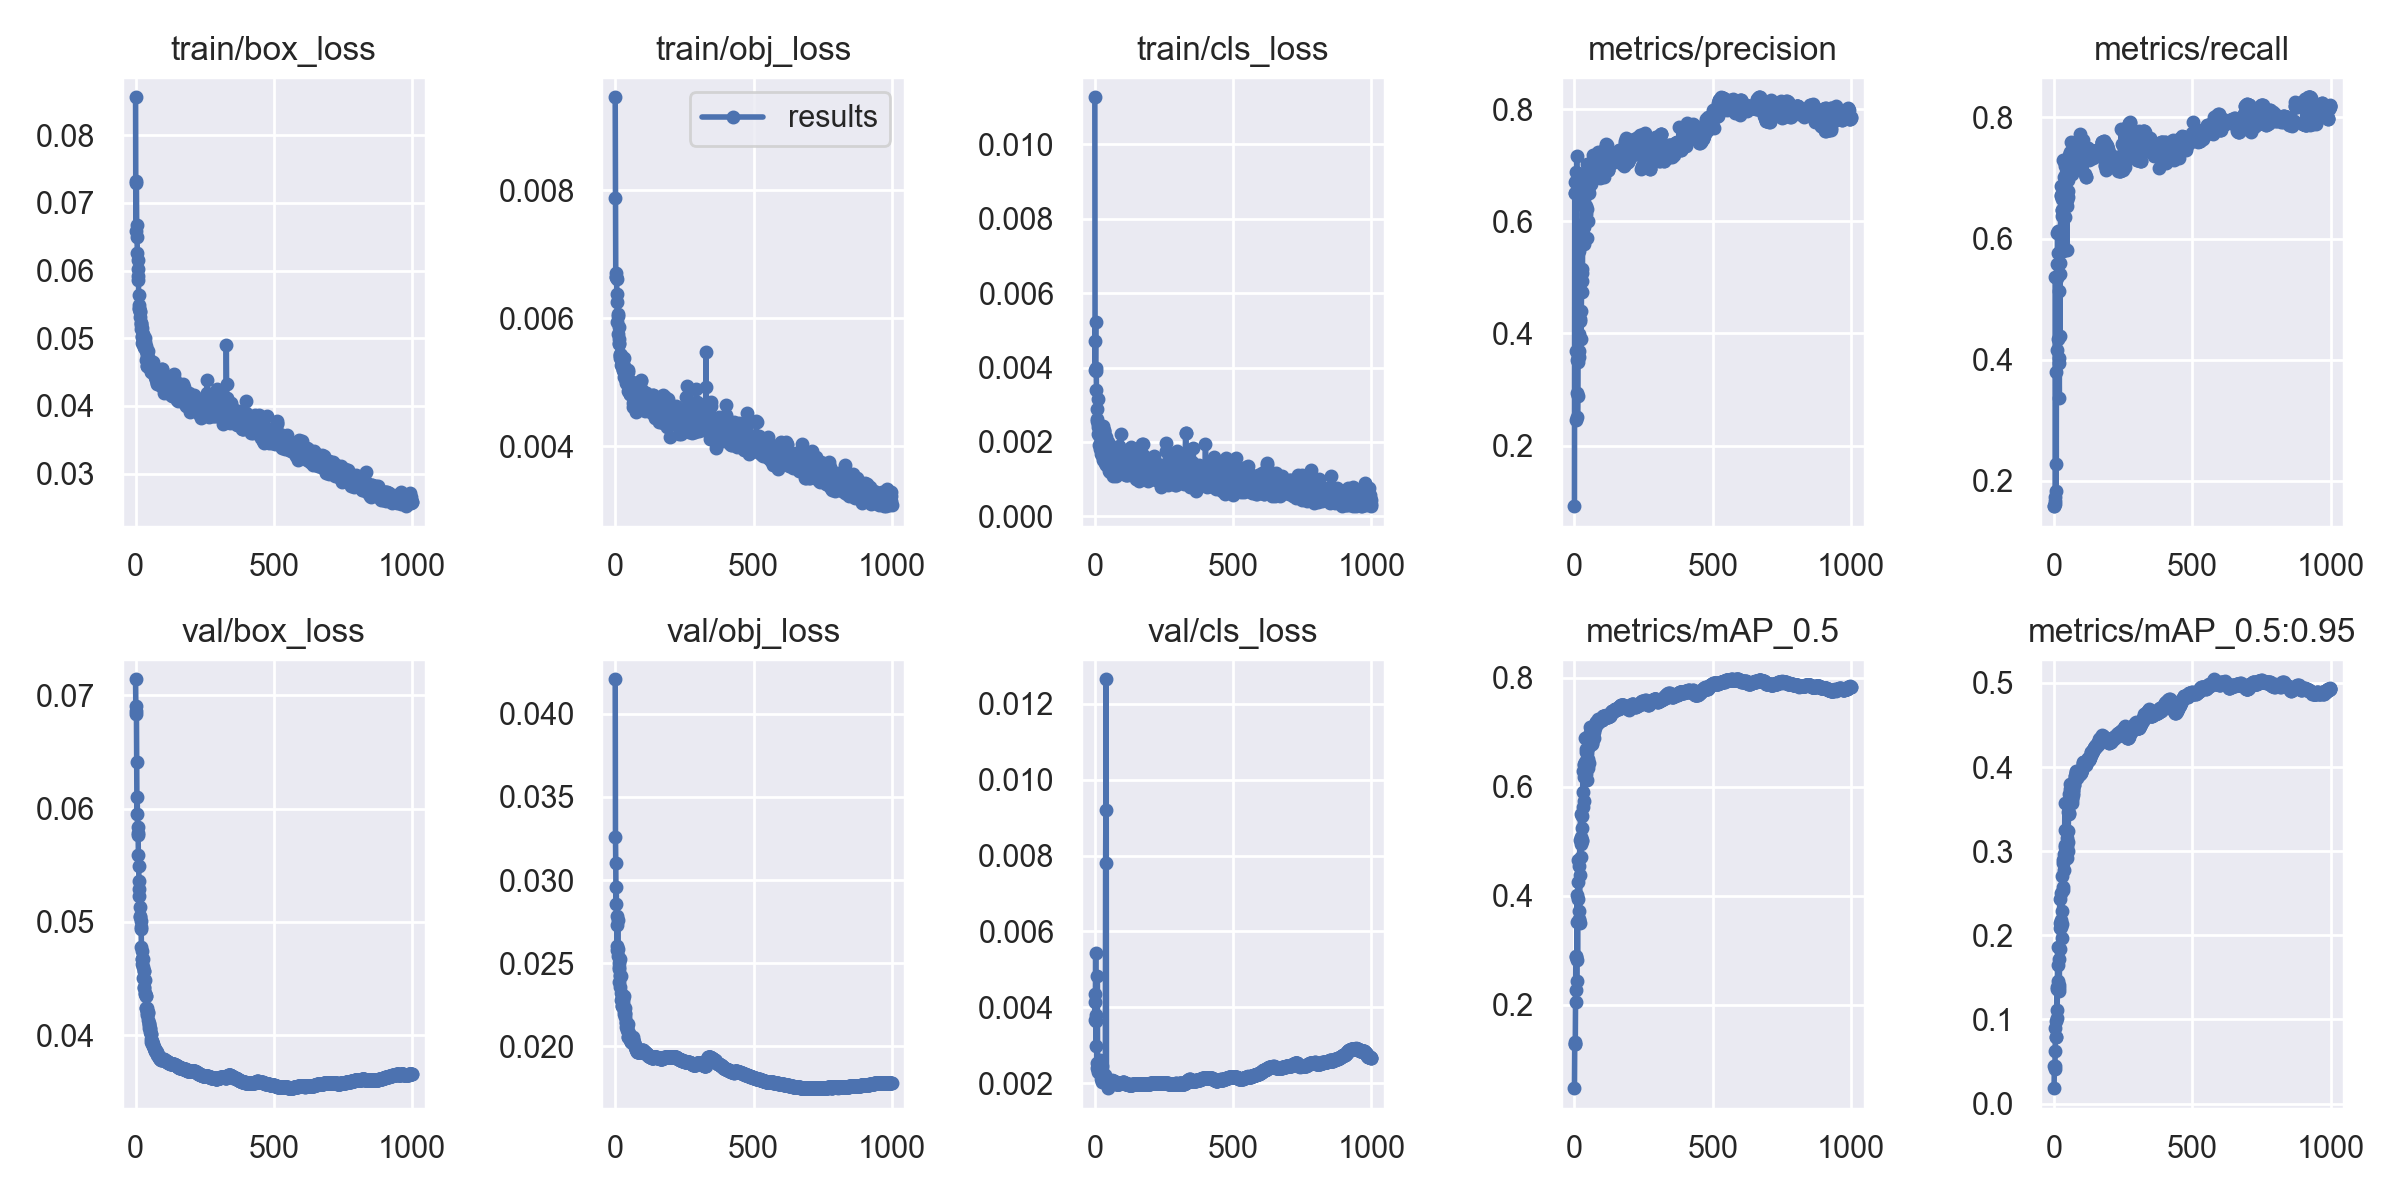
\includegraphics[width=8cm]{Images/YOLOv5L/results.png}
    \caption{Various Results}
\end{figure}
\begin{figure}[H]
    \centering
    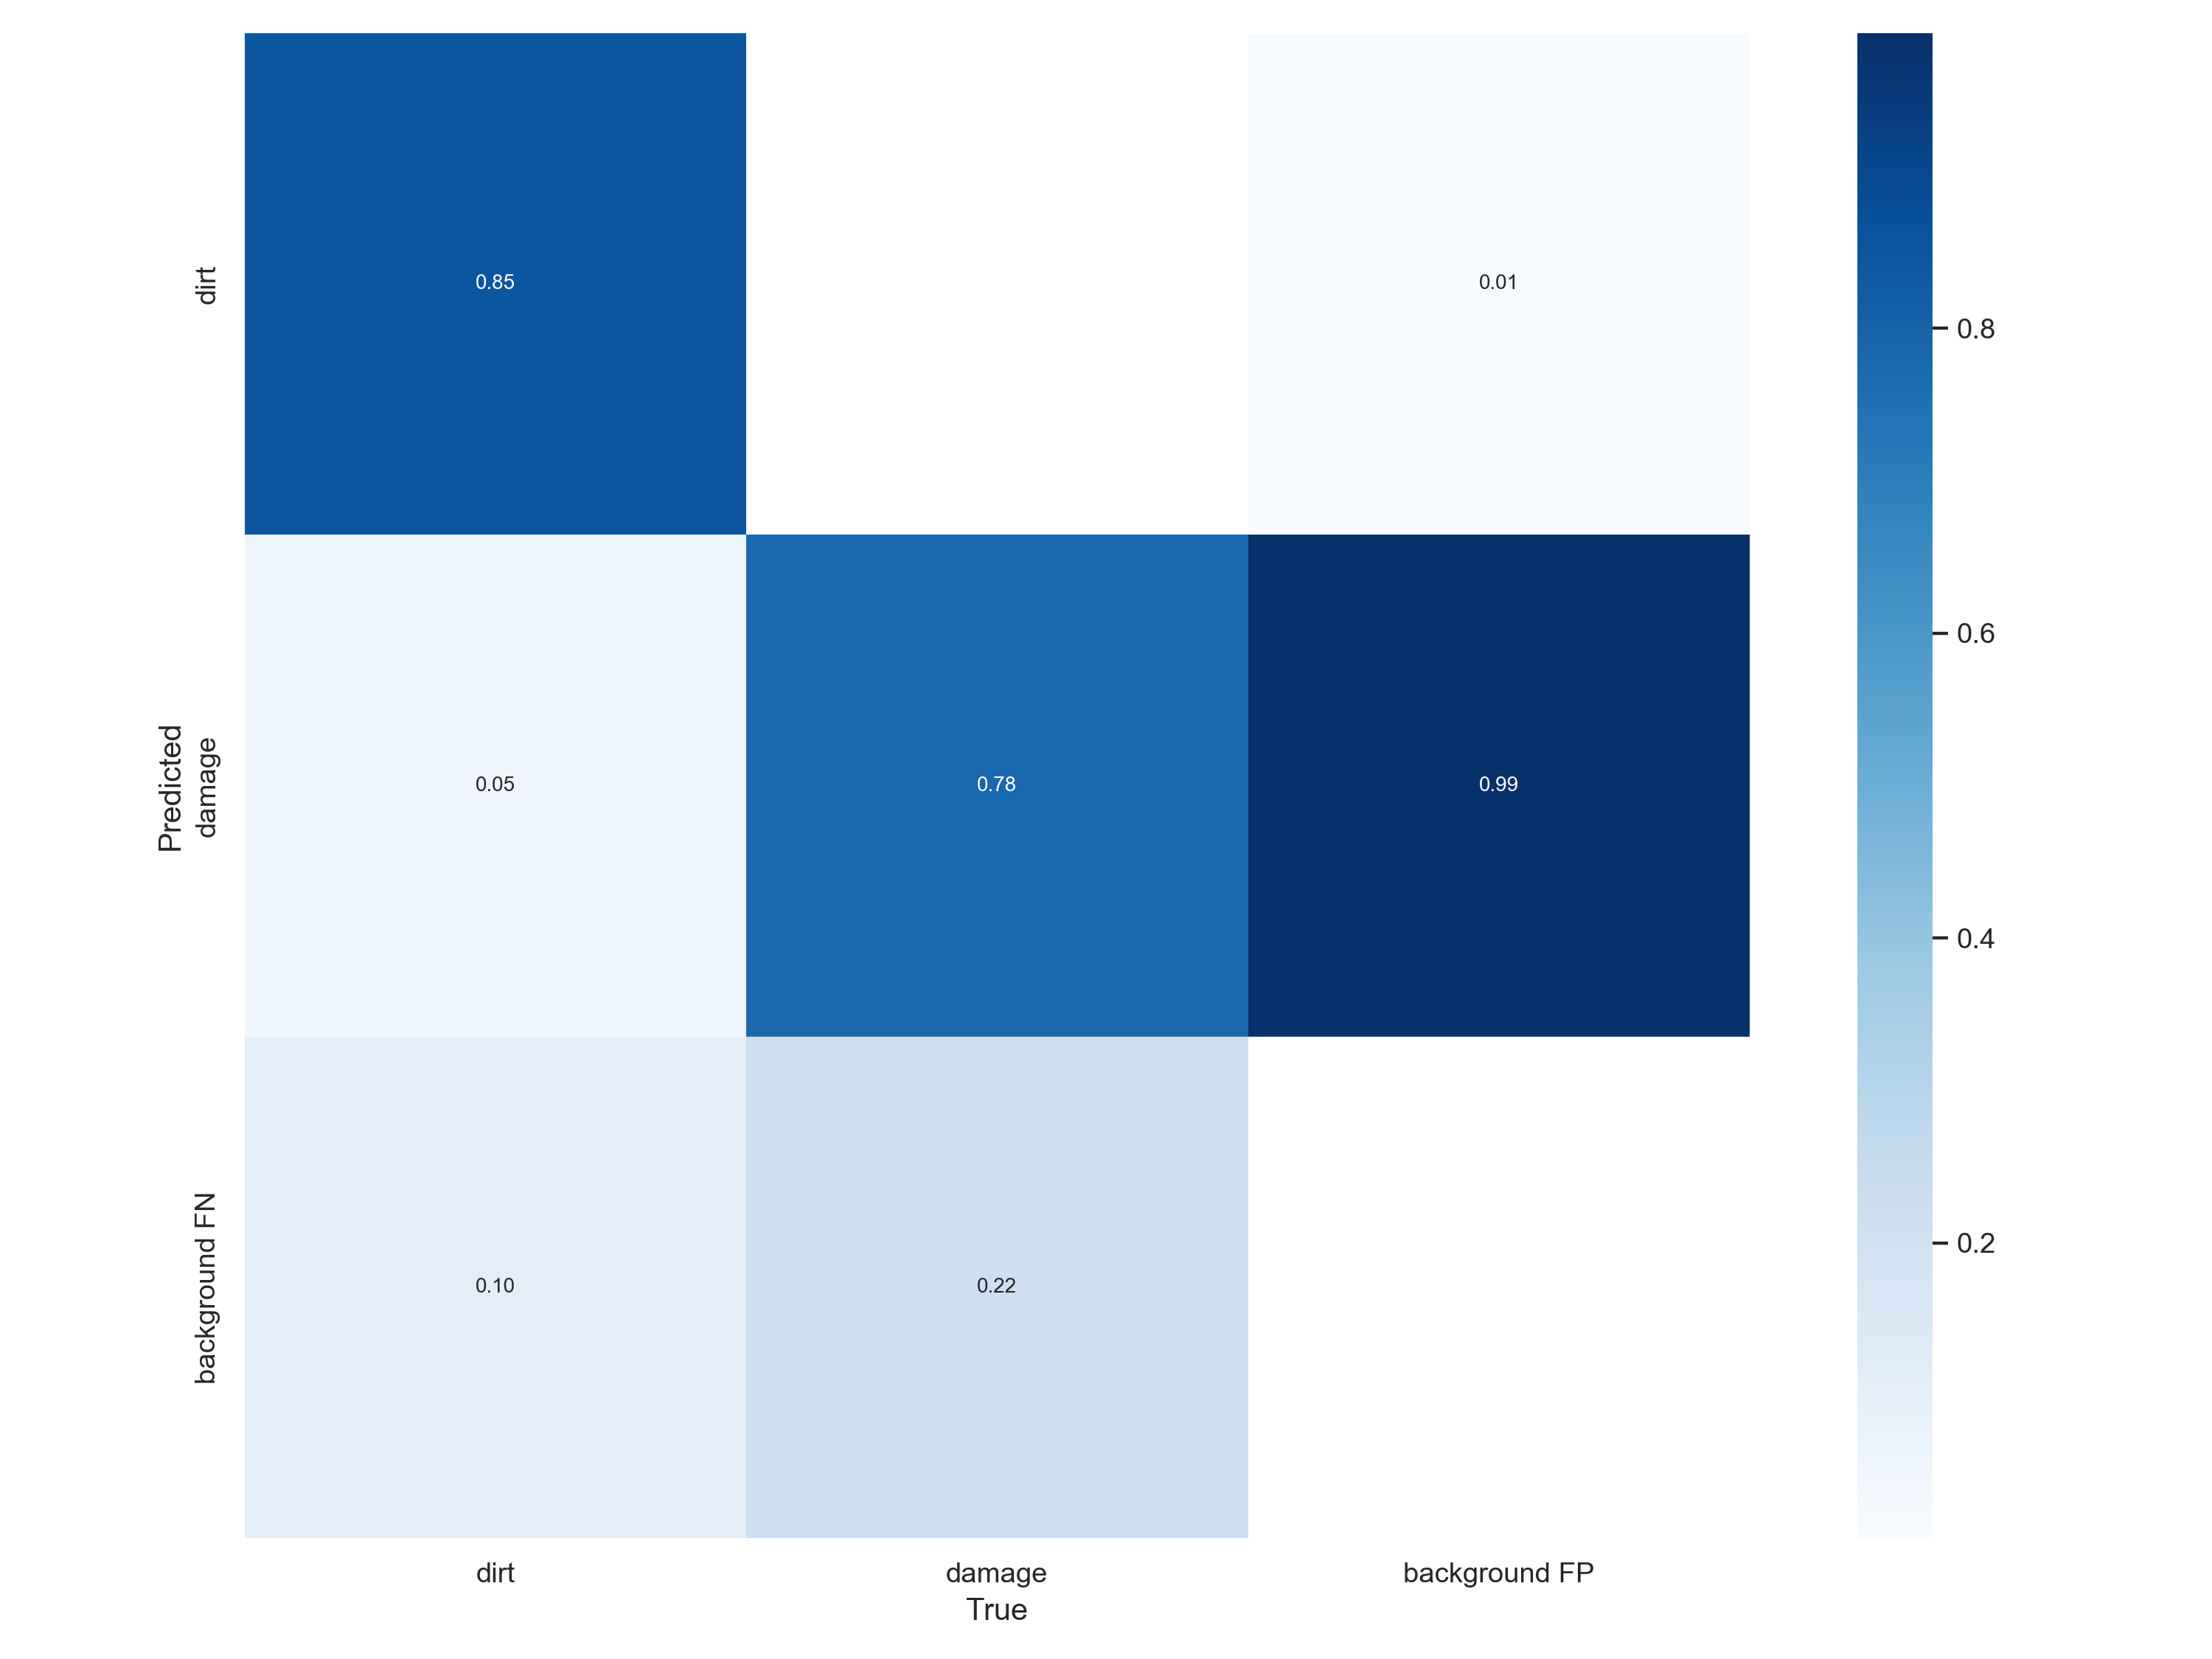
\includegraphics[width=8cm]{Images/Confusion Matrices/Lconfusion_matrix.png}
    \caption{Confusion Matrix}
\end{figure}
\subsection{Augmented training batches}
\begin{figure}[H]
    \centering
    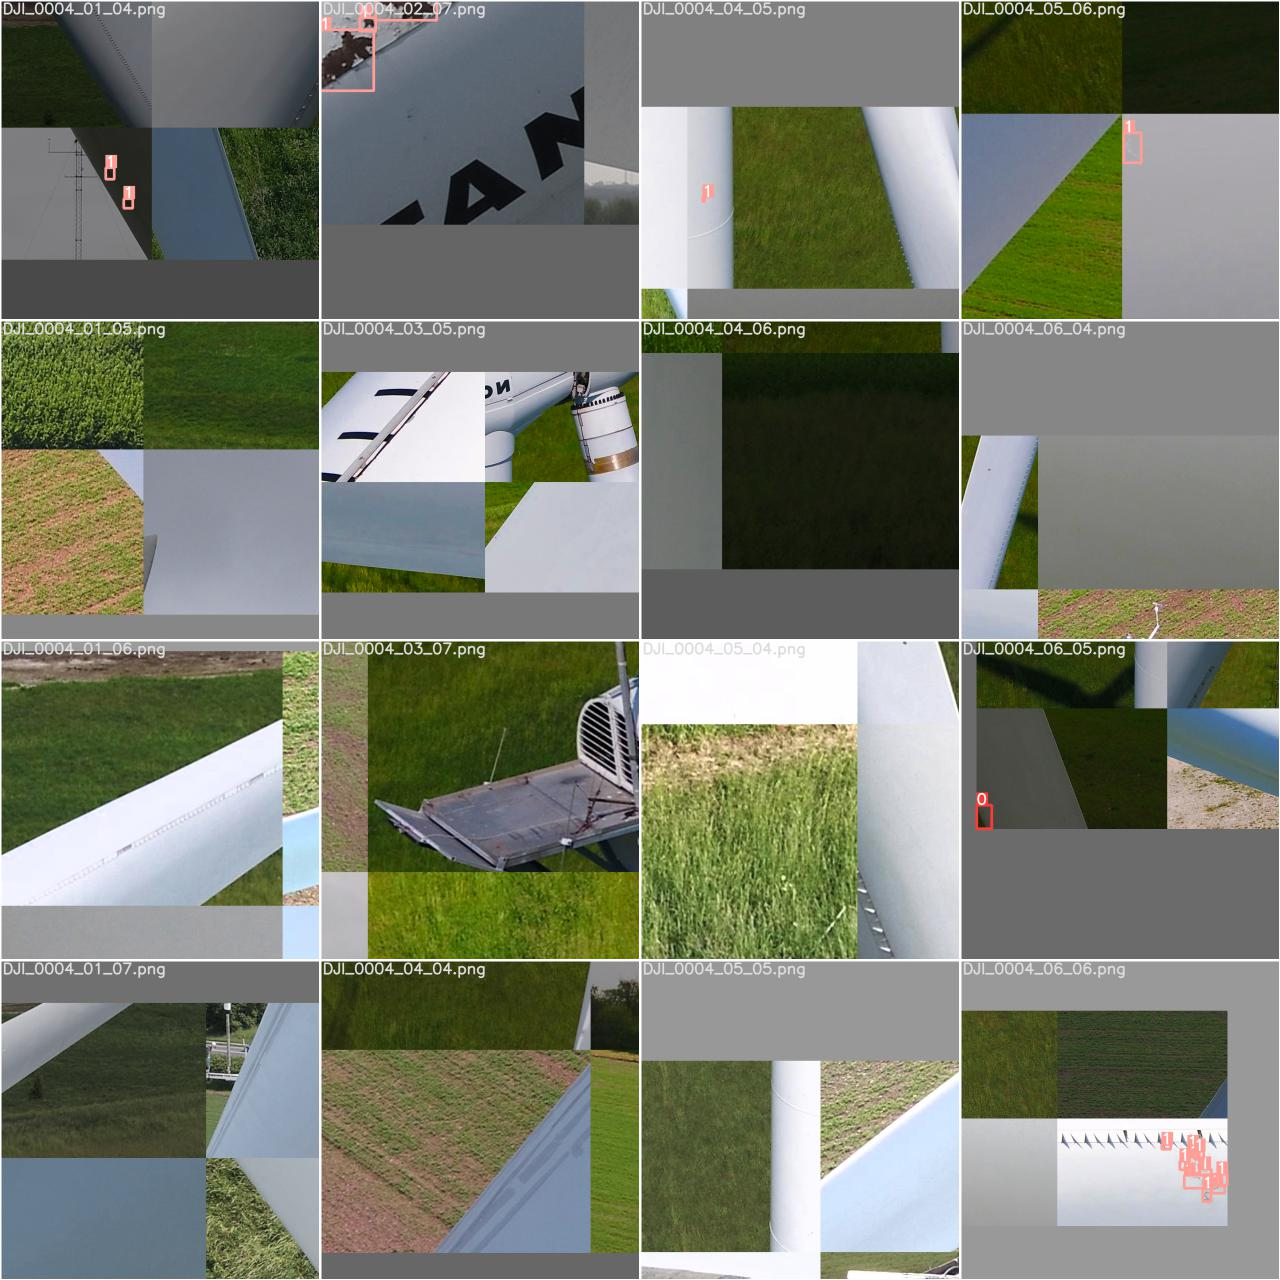
\includegraphics[width=8cm]{Images/YOLOv5L/train_batch0.jpg}
    \caption{Training Batch 0}
\end{figure}
\begin{figure}[H]
    \centering
    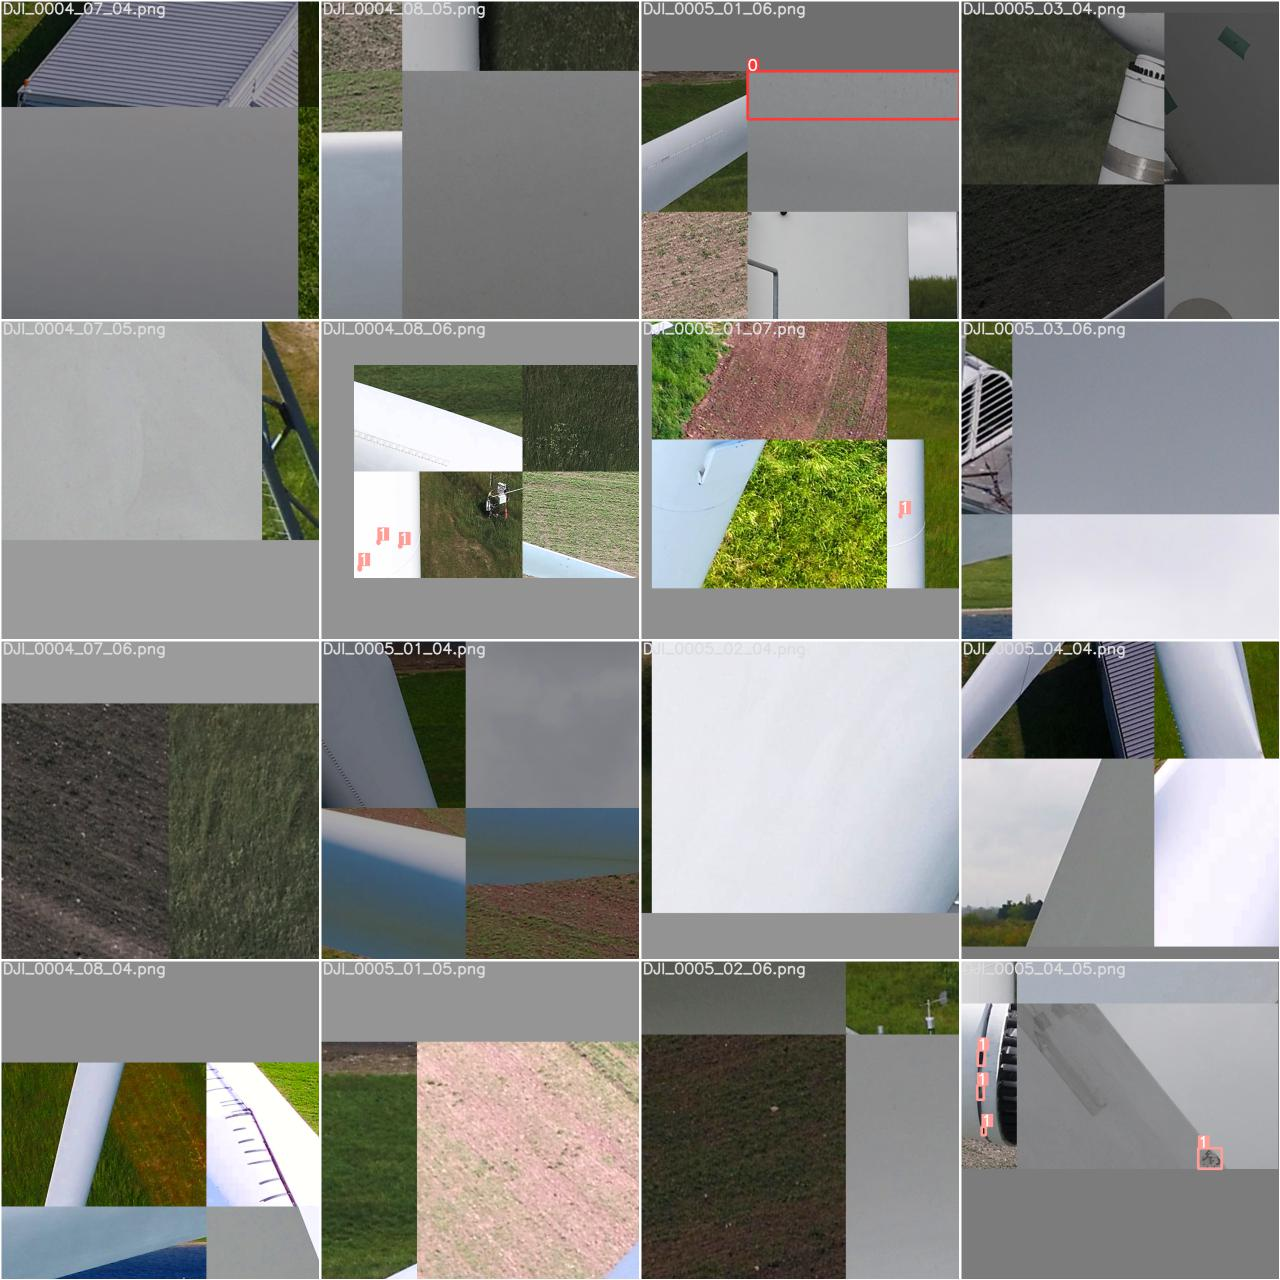
\includegraphics[width=8cm]{Images/YOLOv5L/train_batch1.jpg}
    \caption{Training Batch 1}
\end{figure}
\begin{figure}[H]
    \centering
    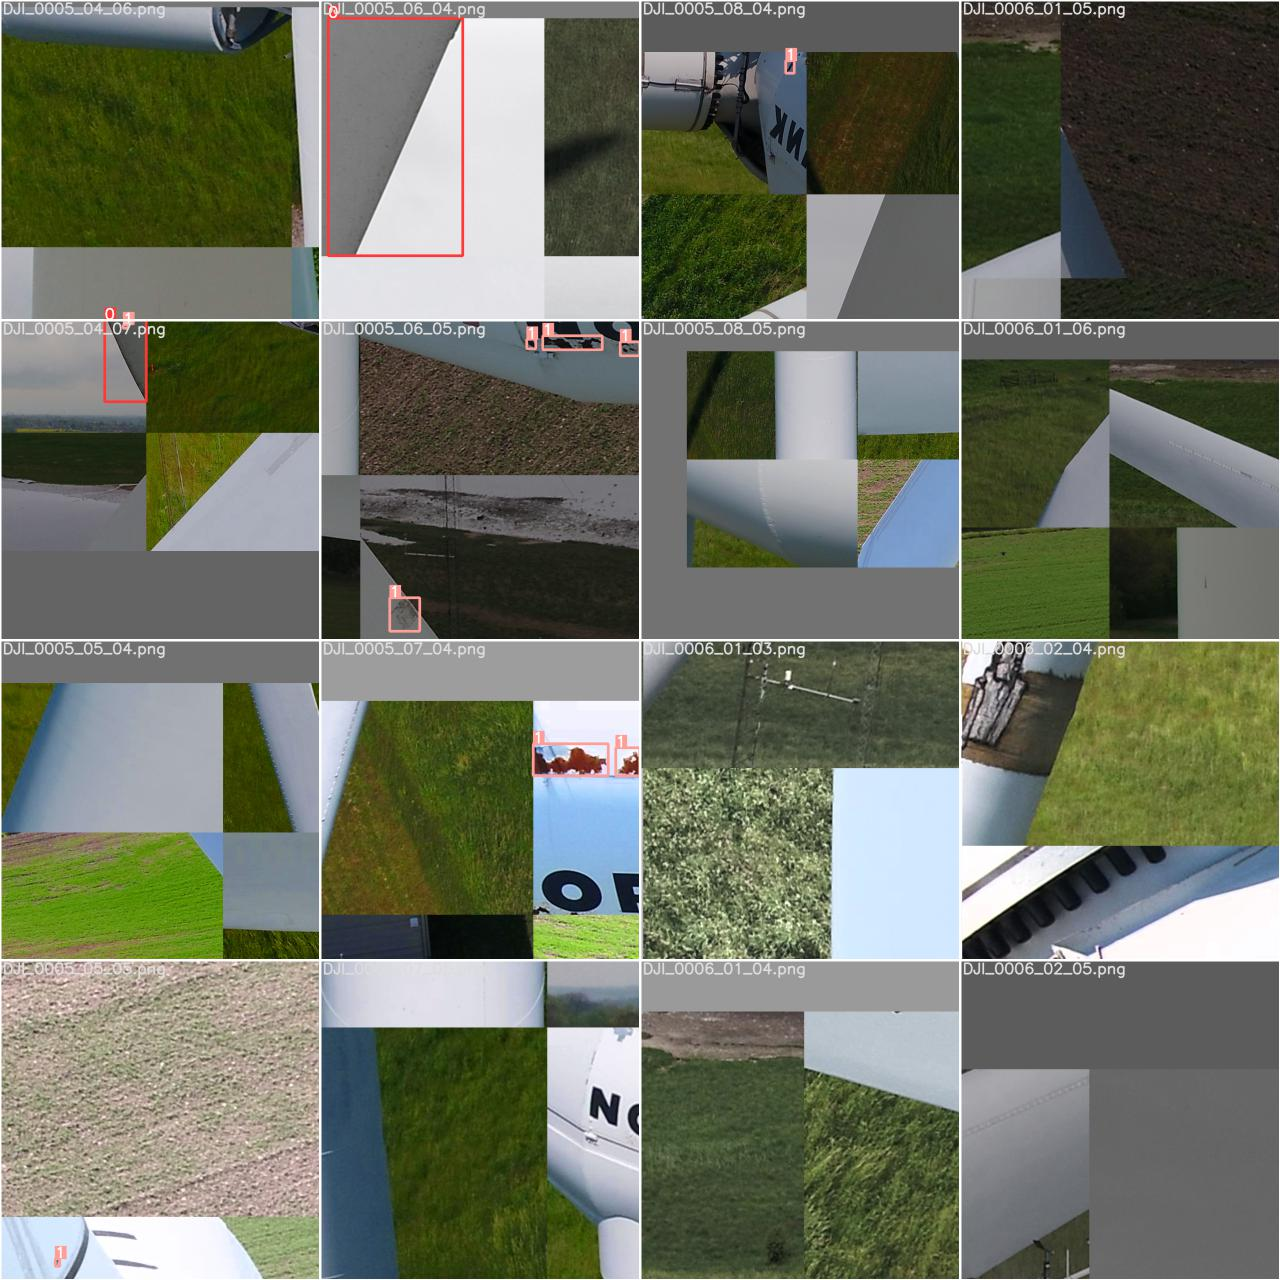
\includegraphics[width=8cm]{Images/YOLOv5L/train_batch2.jpg}
    \caption{Training Batch 2}
\end{figure}
\subsection{Validation batches}
\begin{figure}[H]
    \centering
    \includegraphics[width=8cm]{Images/YOLOv5L/val_batch0_labels.jpg}
    \caption{Validation Batch 0 True Bounding Boxes}
\end{figure}
\begin{figure}[H]
    \centering
    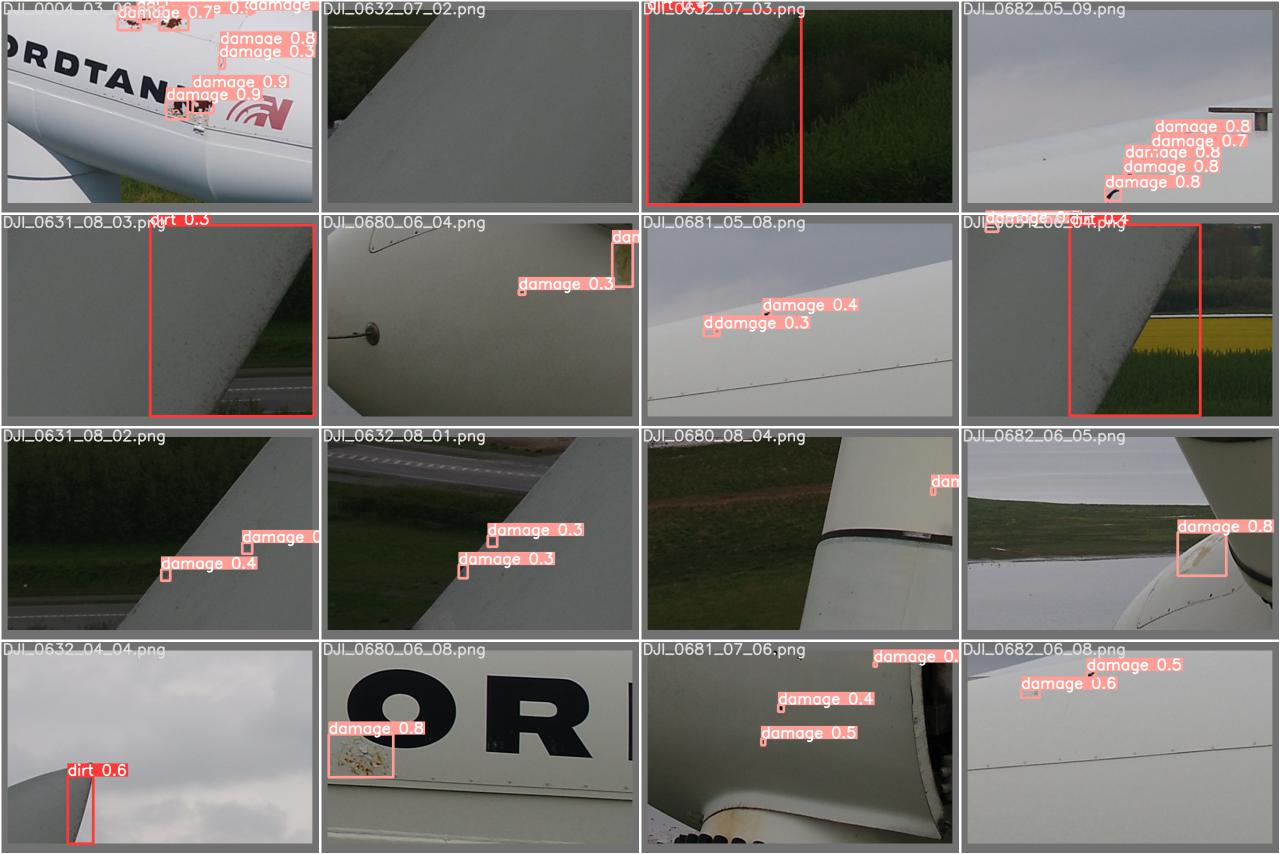
\includegraphics[width=8cm]{Images/YOLOv5L/val_batch0_pred.jpg}
    \caption{Validation Batch 0 Predictions}
\end{figure}
\begin{figure}[H]
    \centering
    \includegraphics[width=8cm]{Images/YOLOv5L/val_batch1_labels.jpg}
    \caption{Validation Batch 1 True Bounding Boxes}
\end{figure}
\begin{figure}[H]
    \centering
    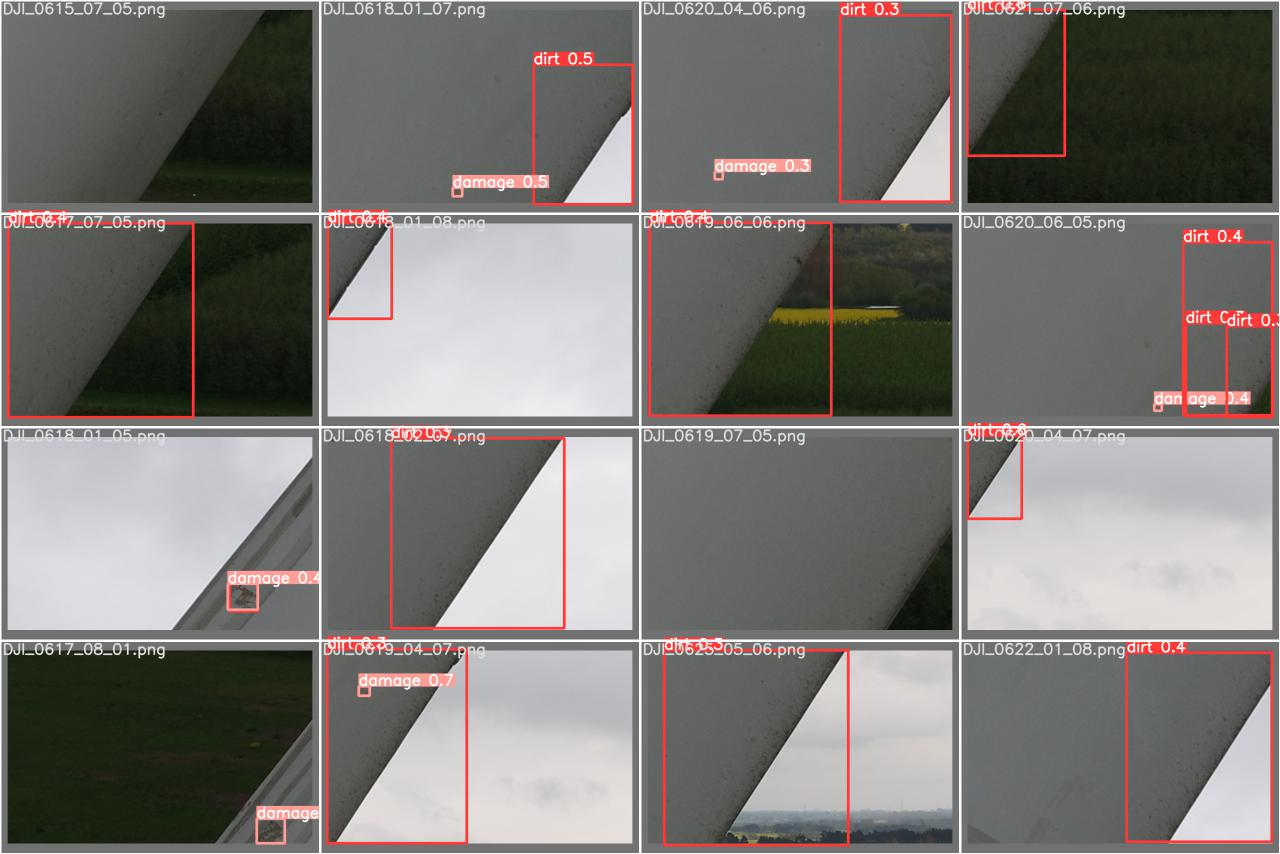
\includegraphics[width=8cm]{Images/YOLOv5L/val_batch1_pred.jpg}
    \caption{Validation Batch 1 Predictions}
\end{figure}
\begin{figure}[H]
    \centering
    \includegraphics[width=8cm]{Images/YOLOv5L/val_batch2_labels.jpg}
    \caption{Validation Batch 2 True Bounding Boxes}
\end{figure}
\begin{figure}[H]
    \centering
    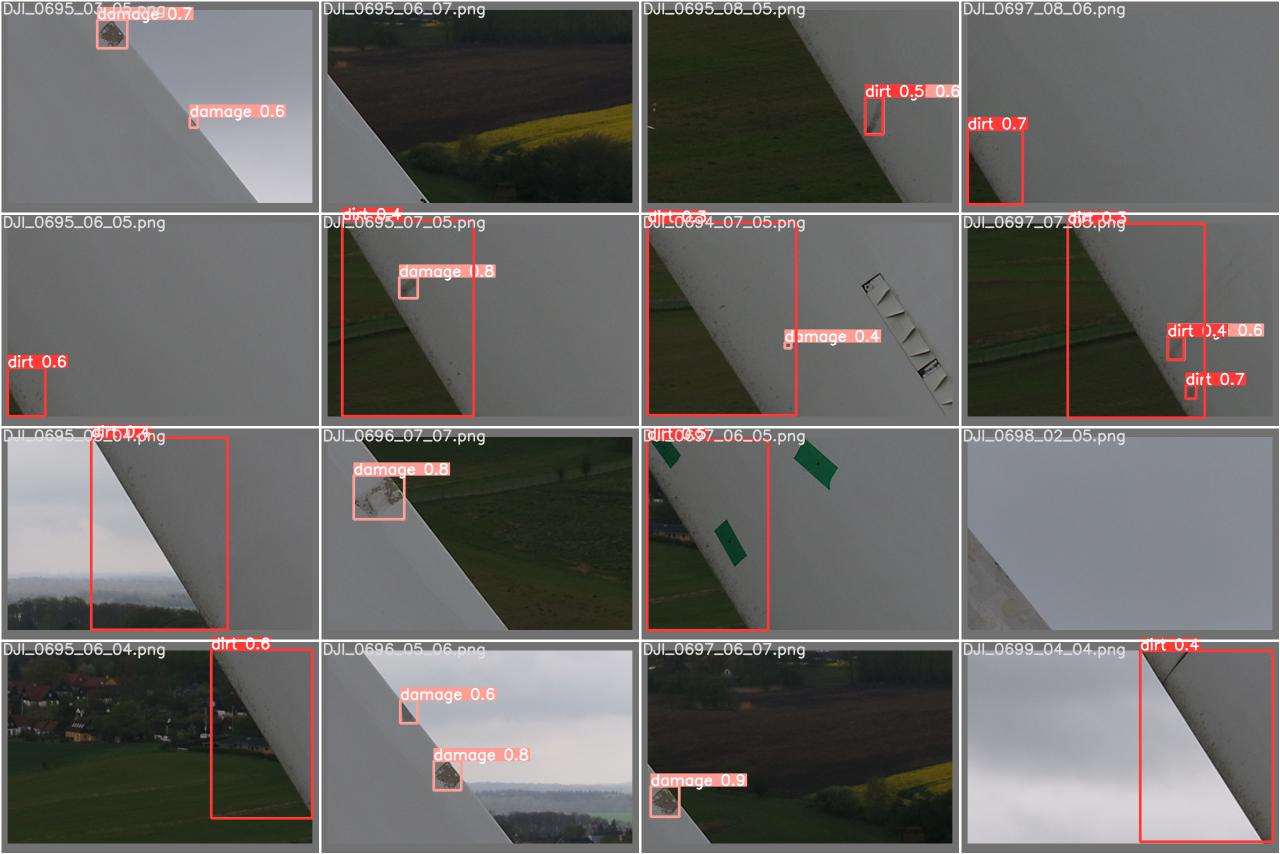
\includegraphics[width=8cm]{Images/YOLOv5L/val_batch2_pred.jpg}
    \caption{Validation Batch 2 Predictions}
\end{figure}
\cleardoublepage
\subsection{YOLOv5m}

\begin{figure}[H]
    \centering
    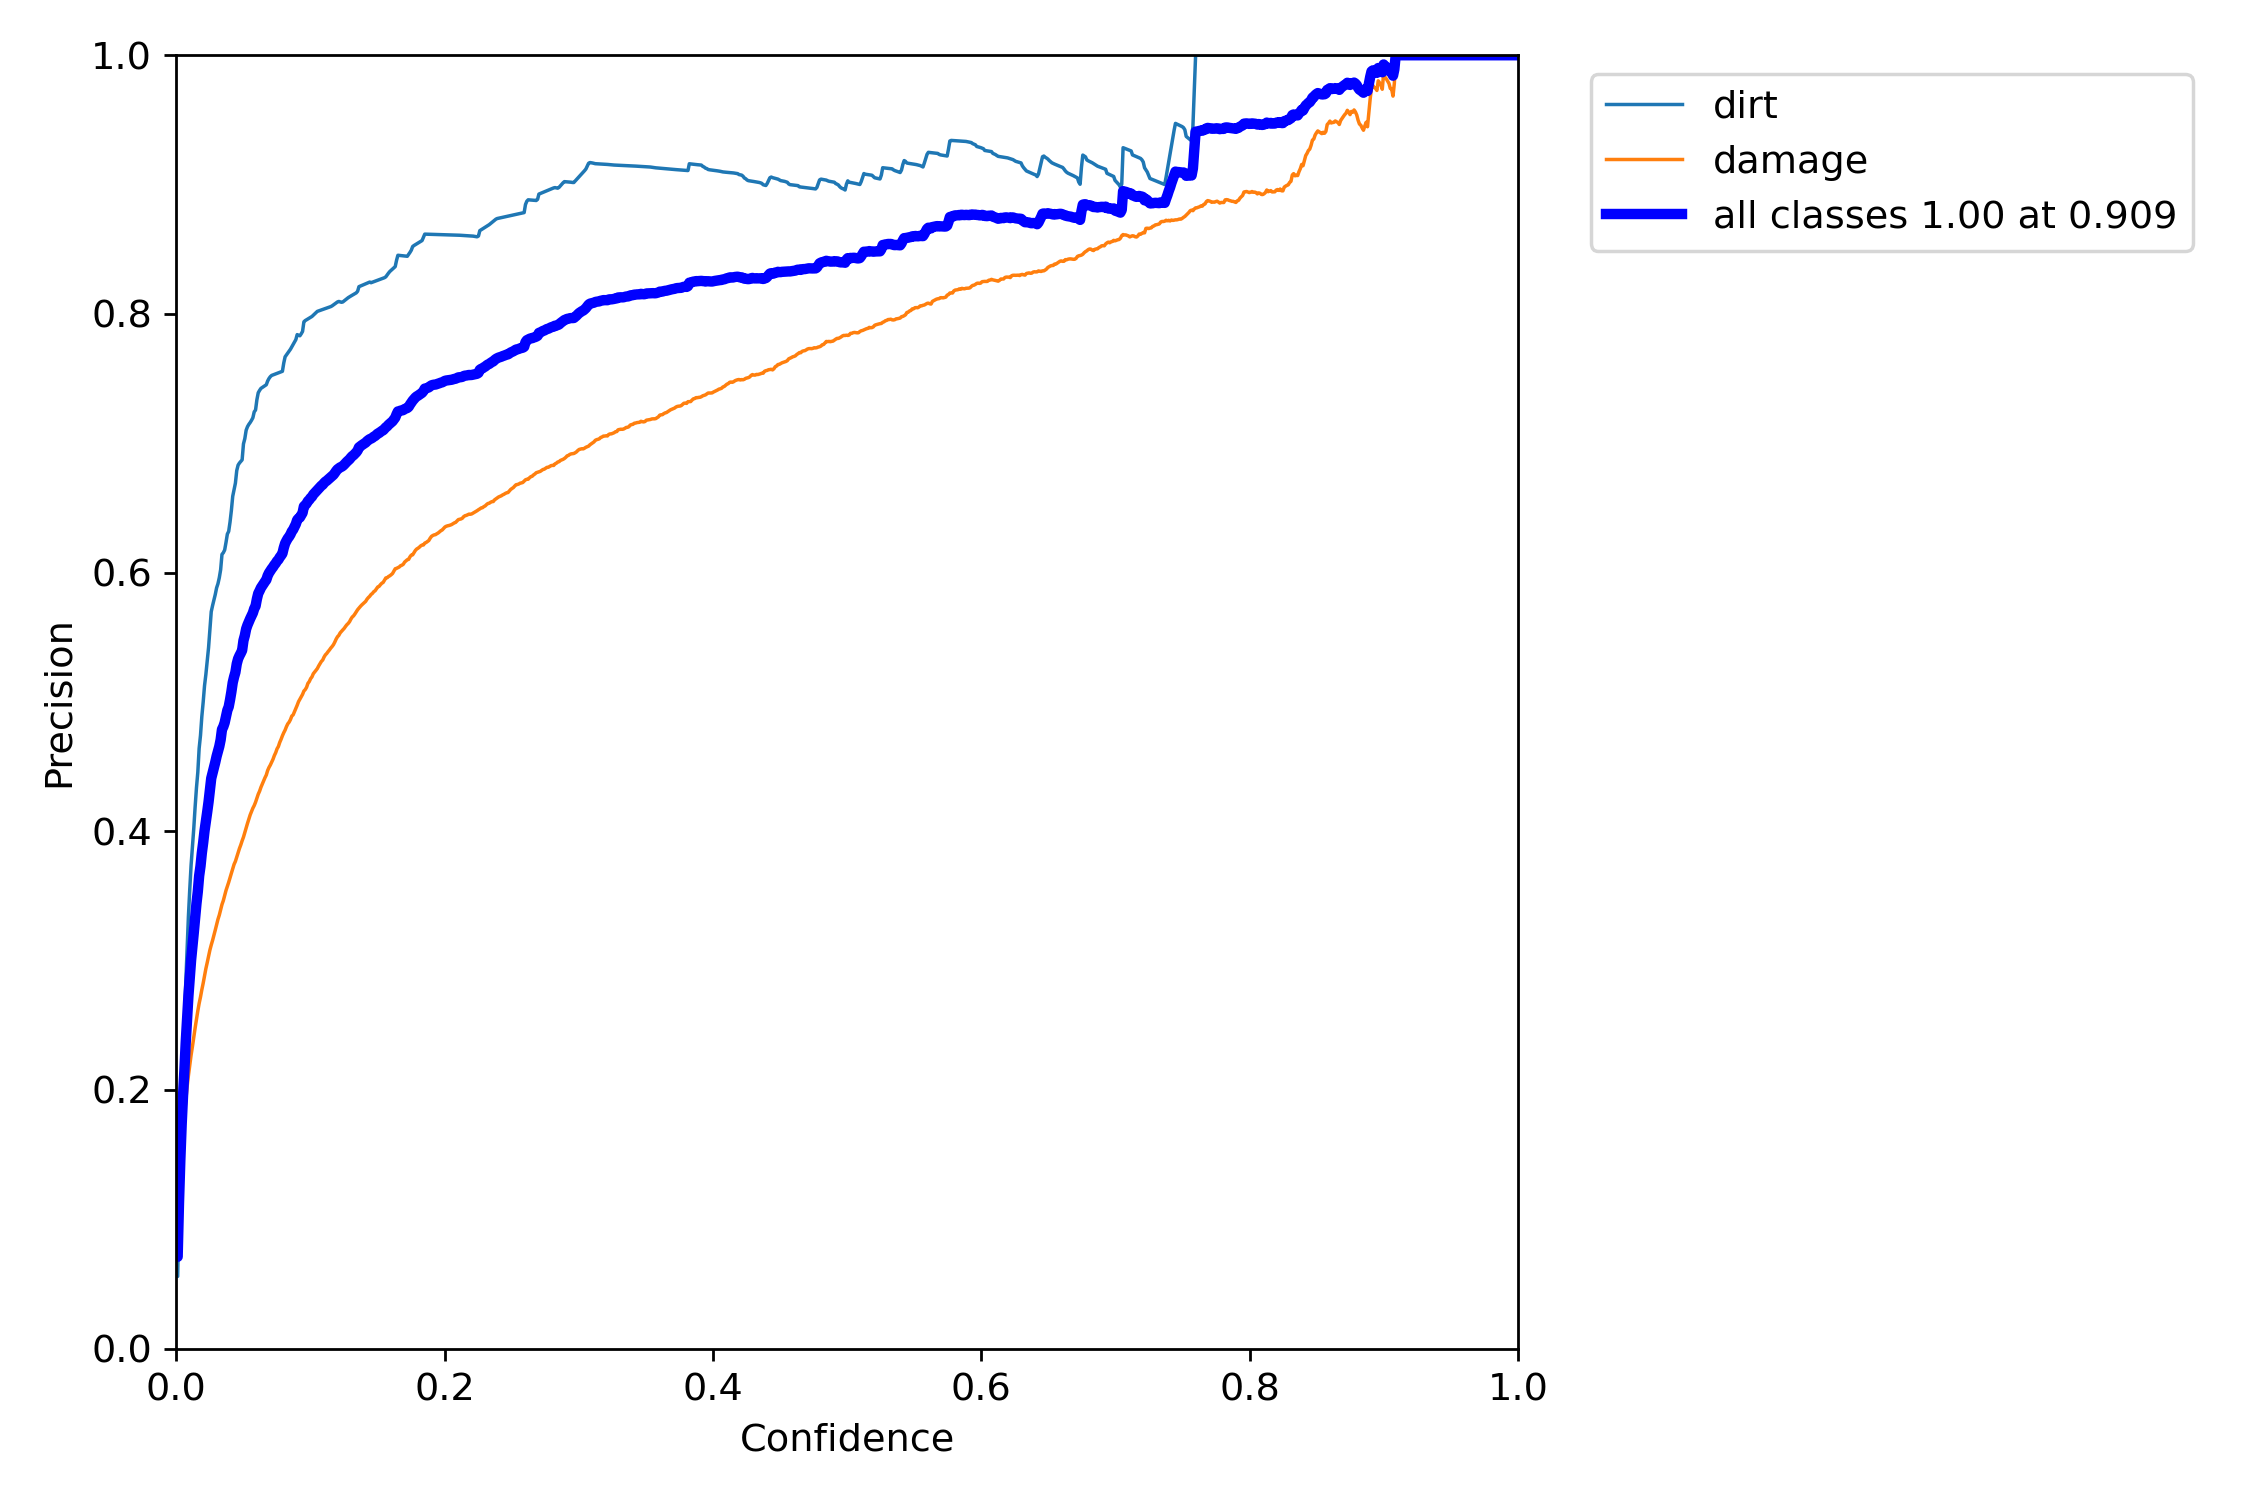
\includegraphics[width=8cm]{Images/YOLOv5m/P_curve.png}
    \caption{Precision-Curve}
\end{figure}
\begin{figure}[H]
    \centering
    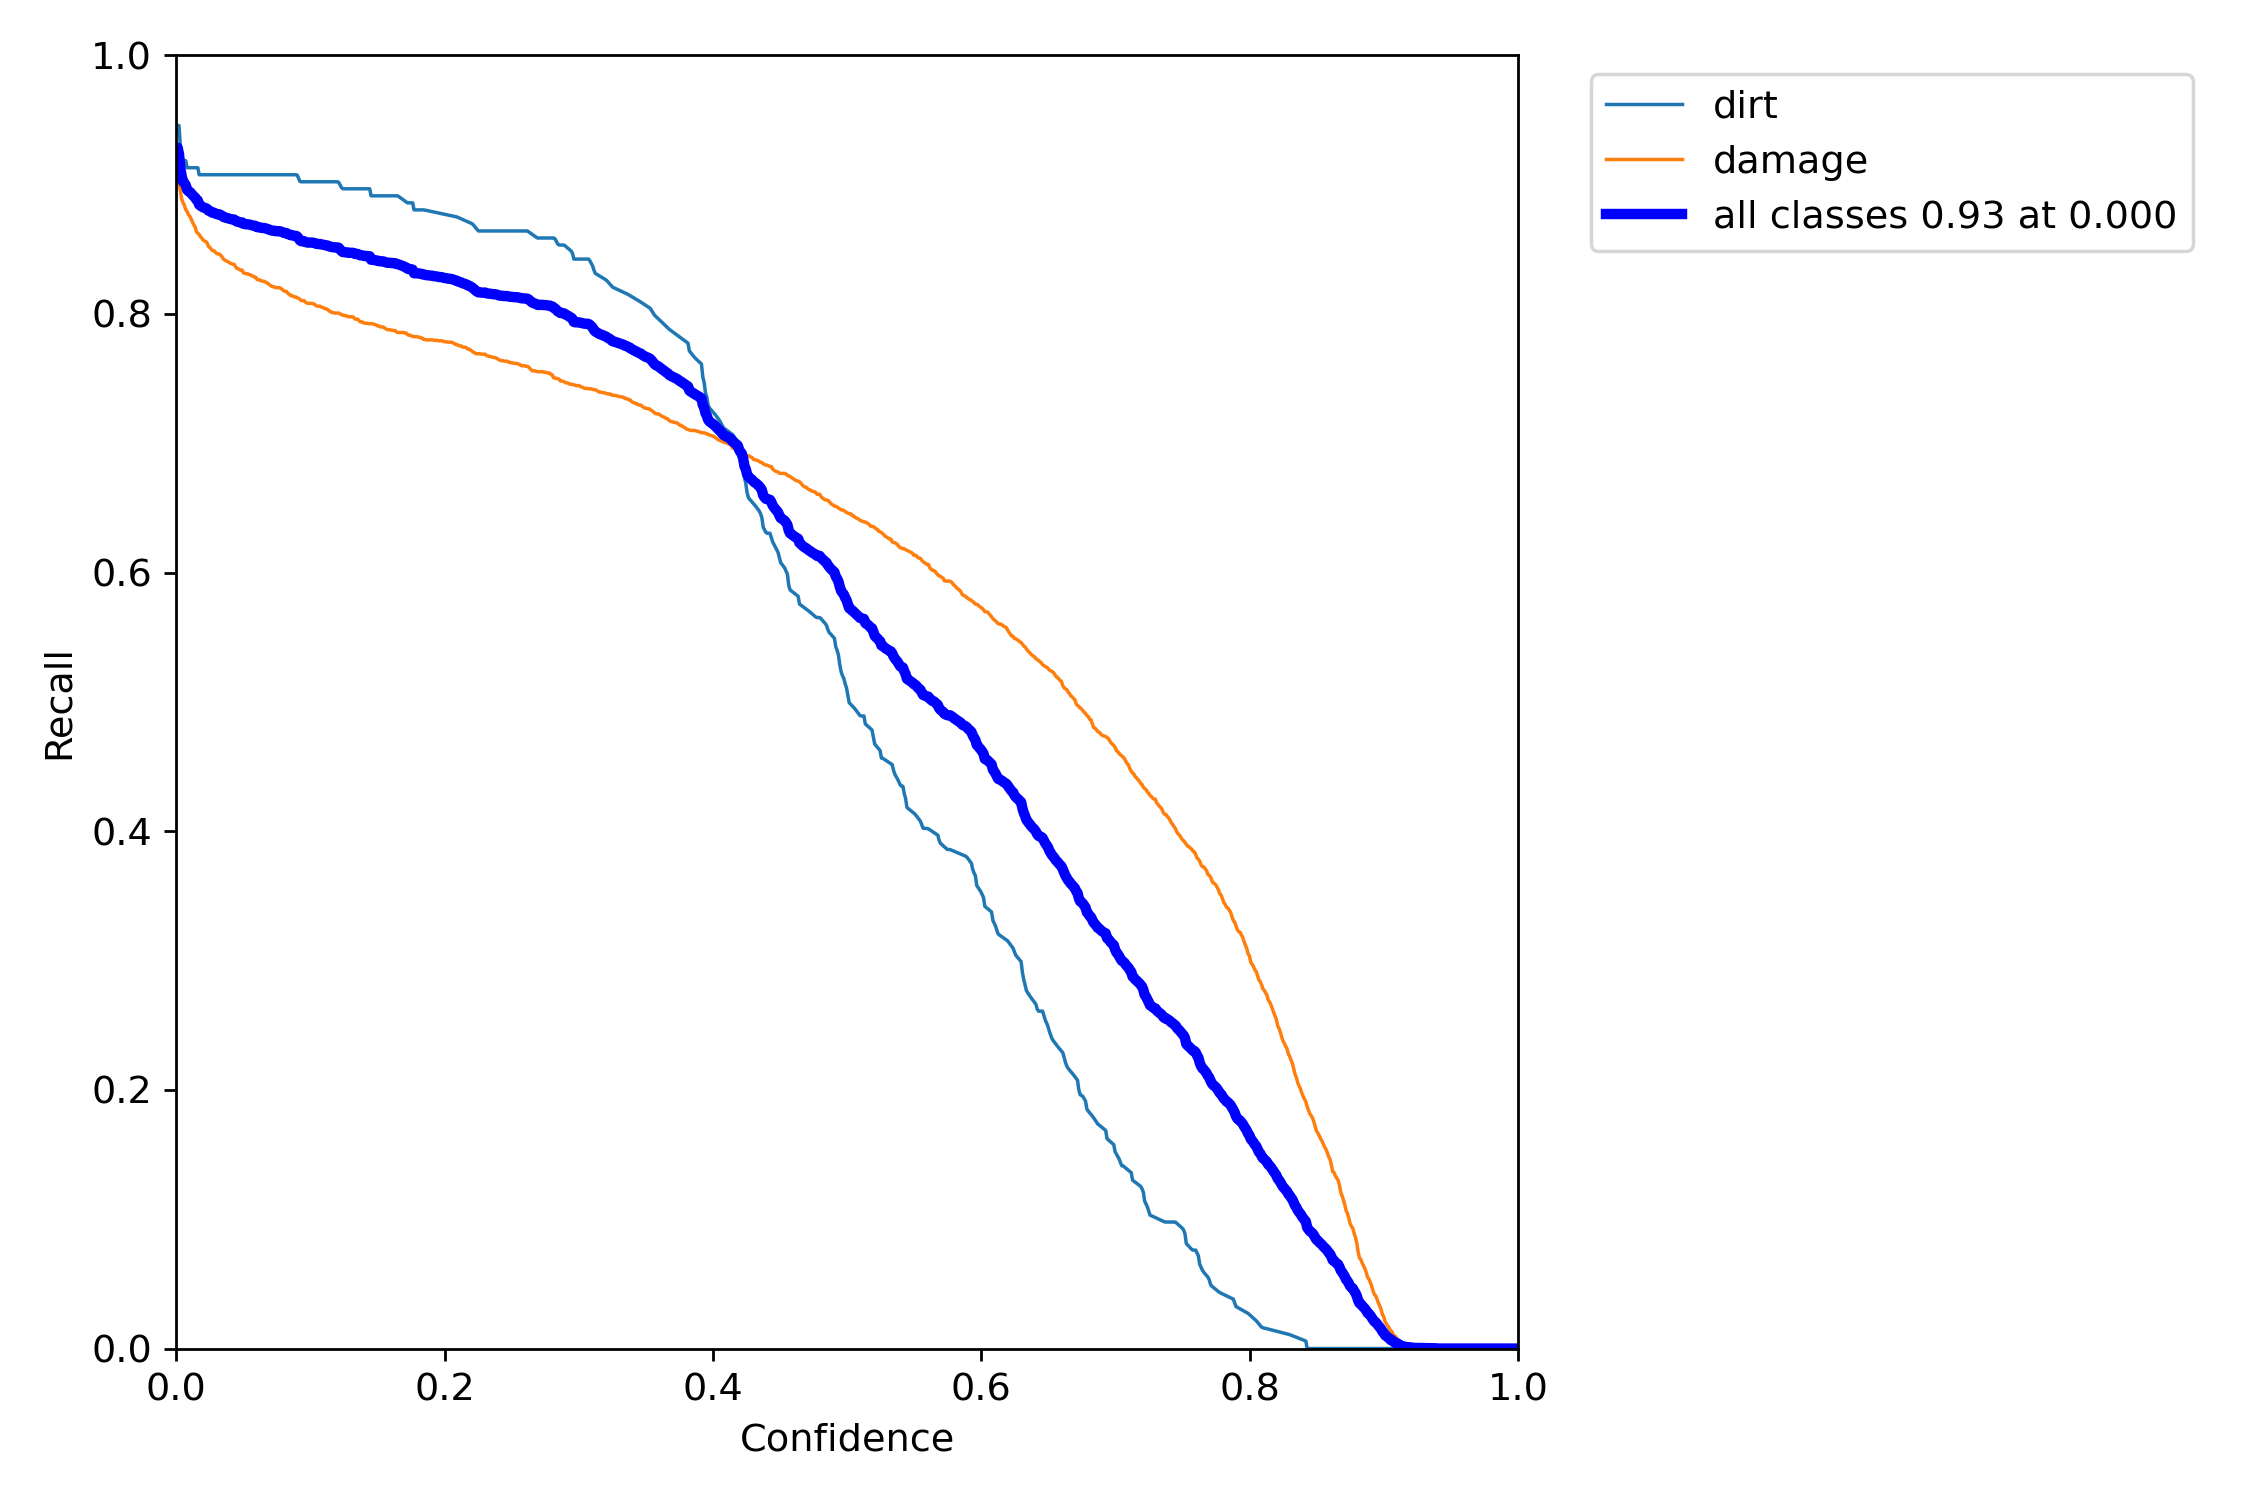
\includegraphics[width=8cm]{Images/YOLOv5m/R_curve.png}
    \caption{Recall-Curve}
\end{figure}
\begin{figure}[H]
    \centering
    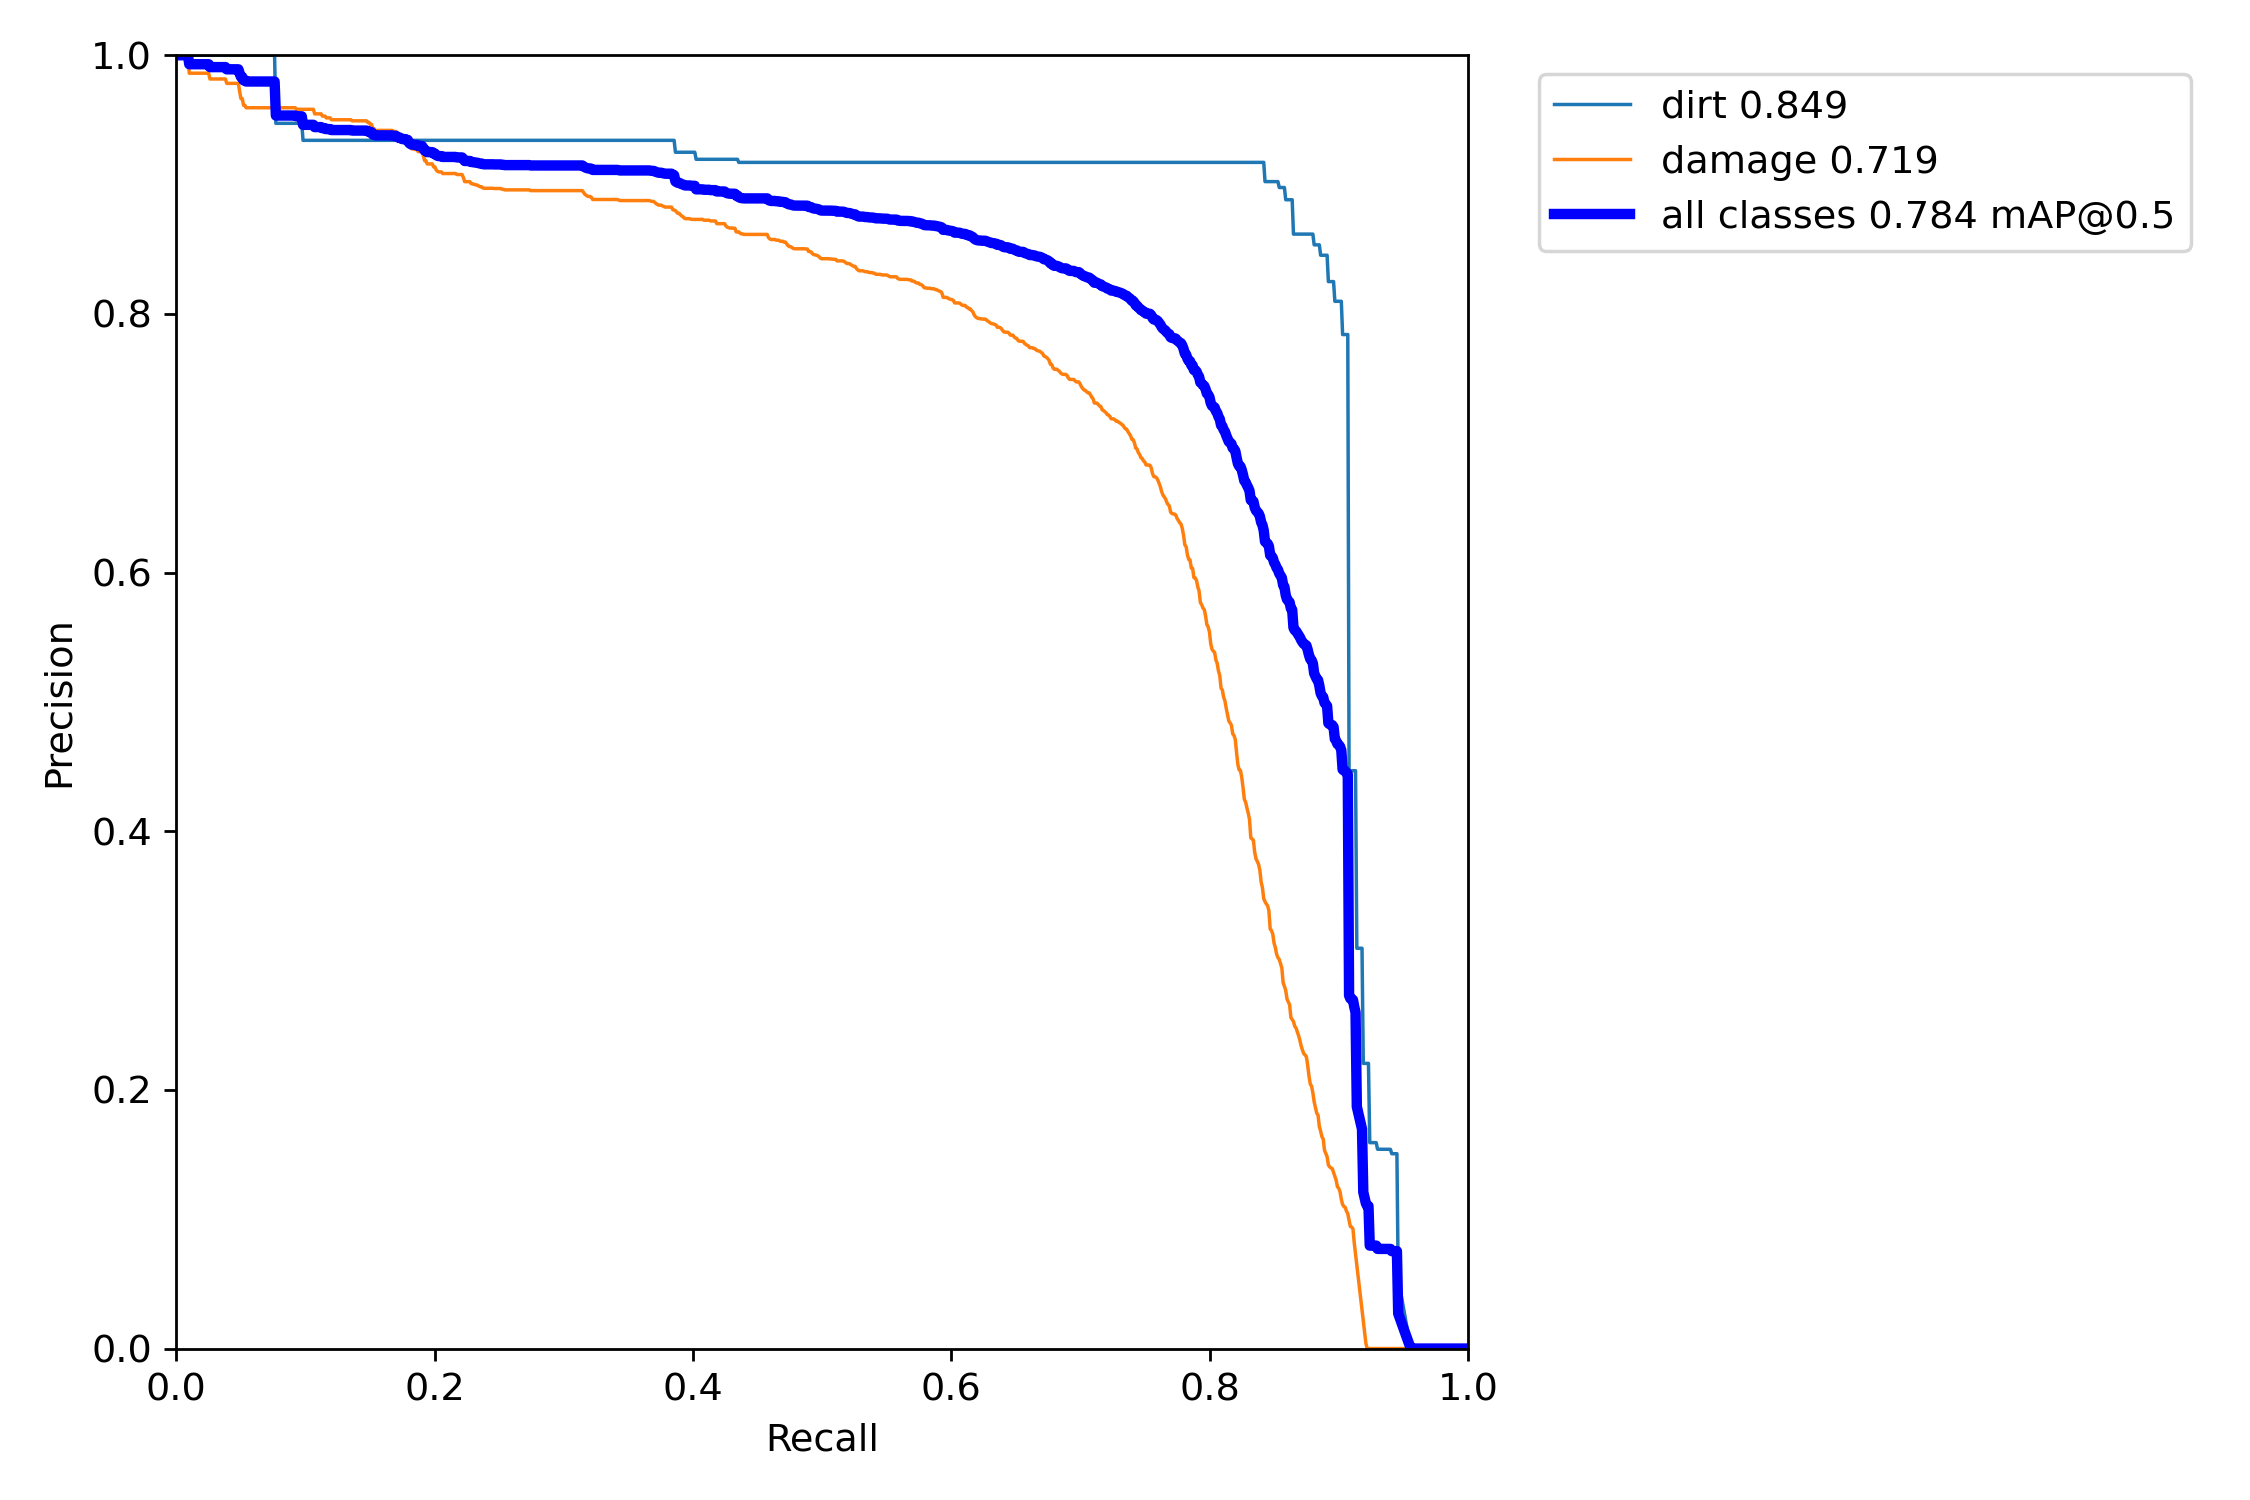
\includegraphics[width=8cm]{Images/YOLOv5m/PR_curve.png}
    \caption{PR-Curve}
\end{figure}
\begin{figure}[H]
    \centering
    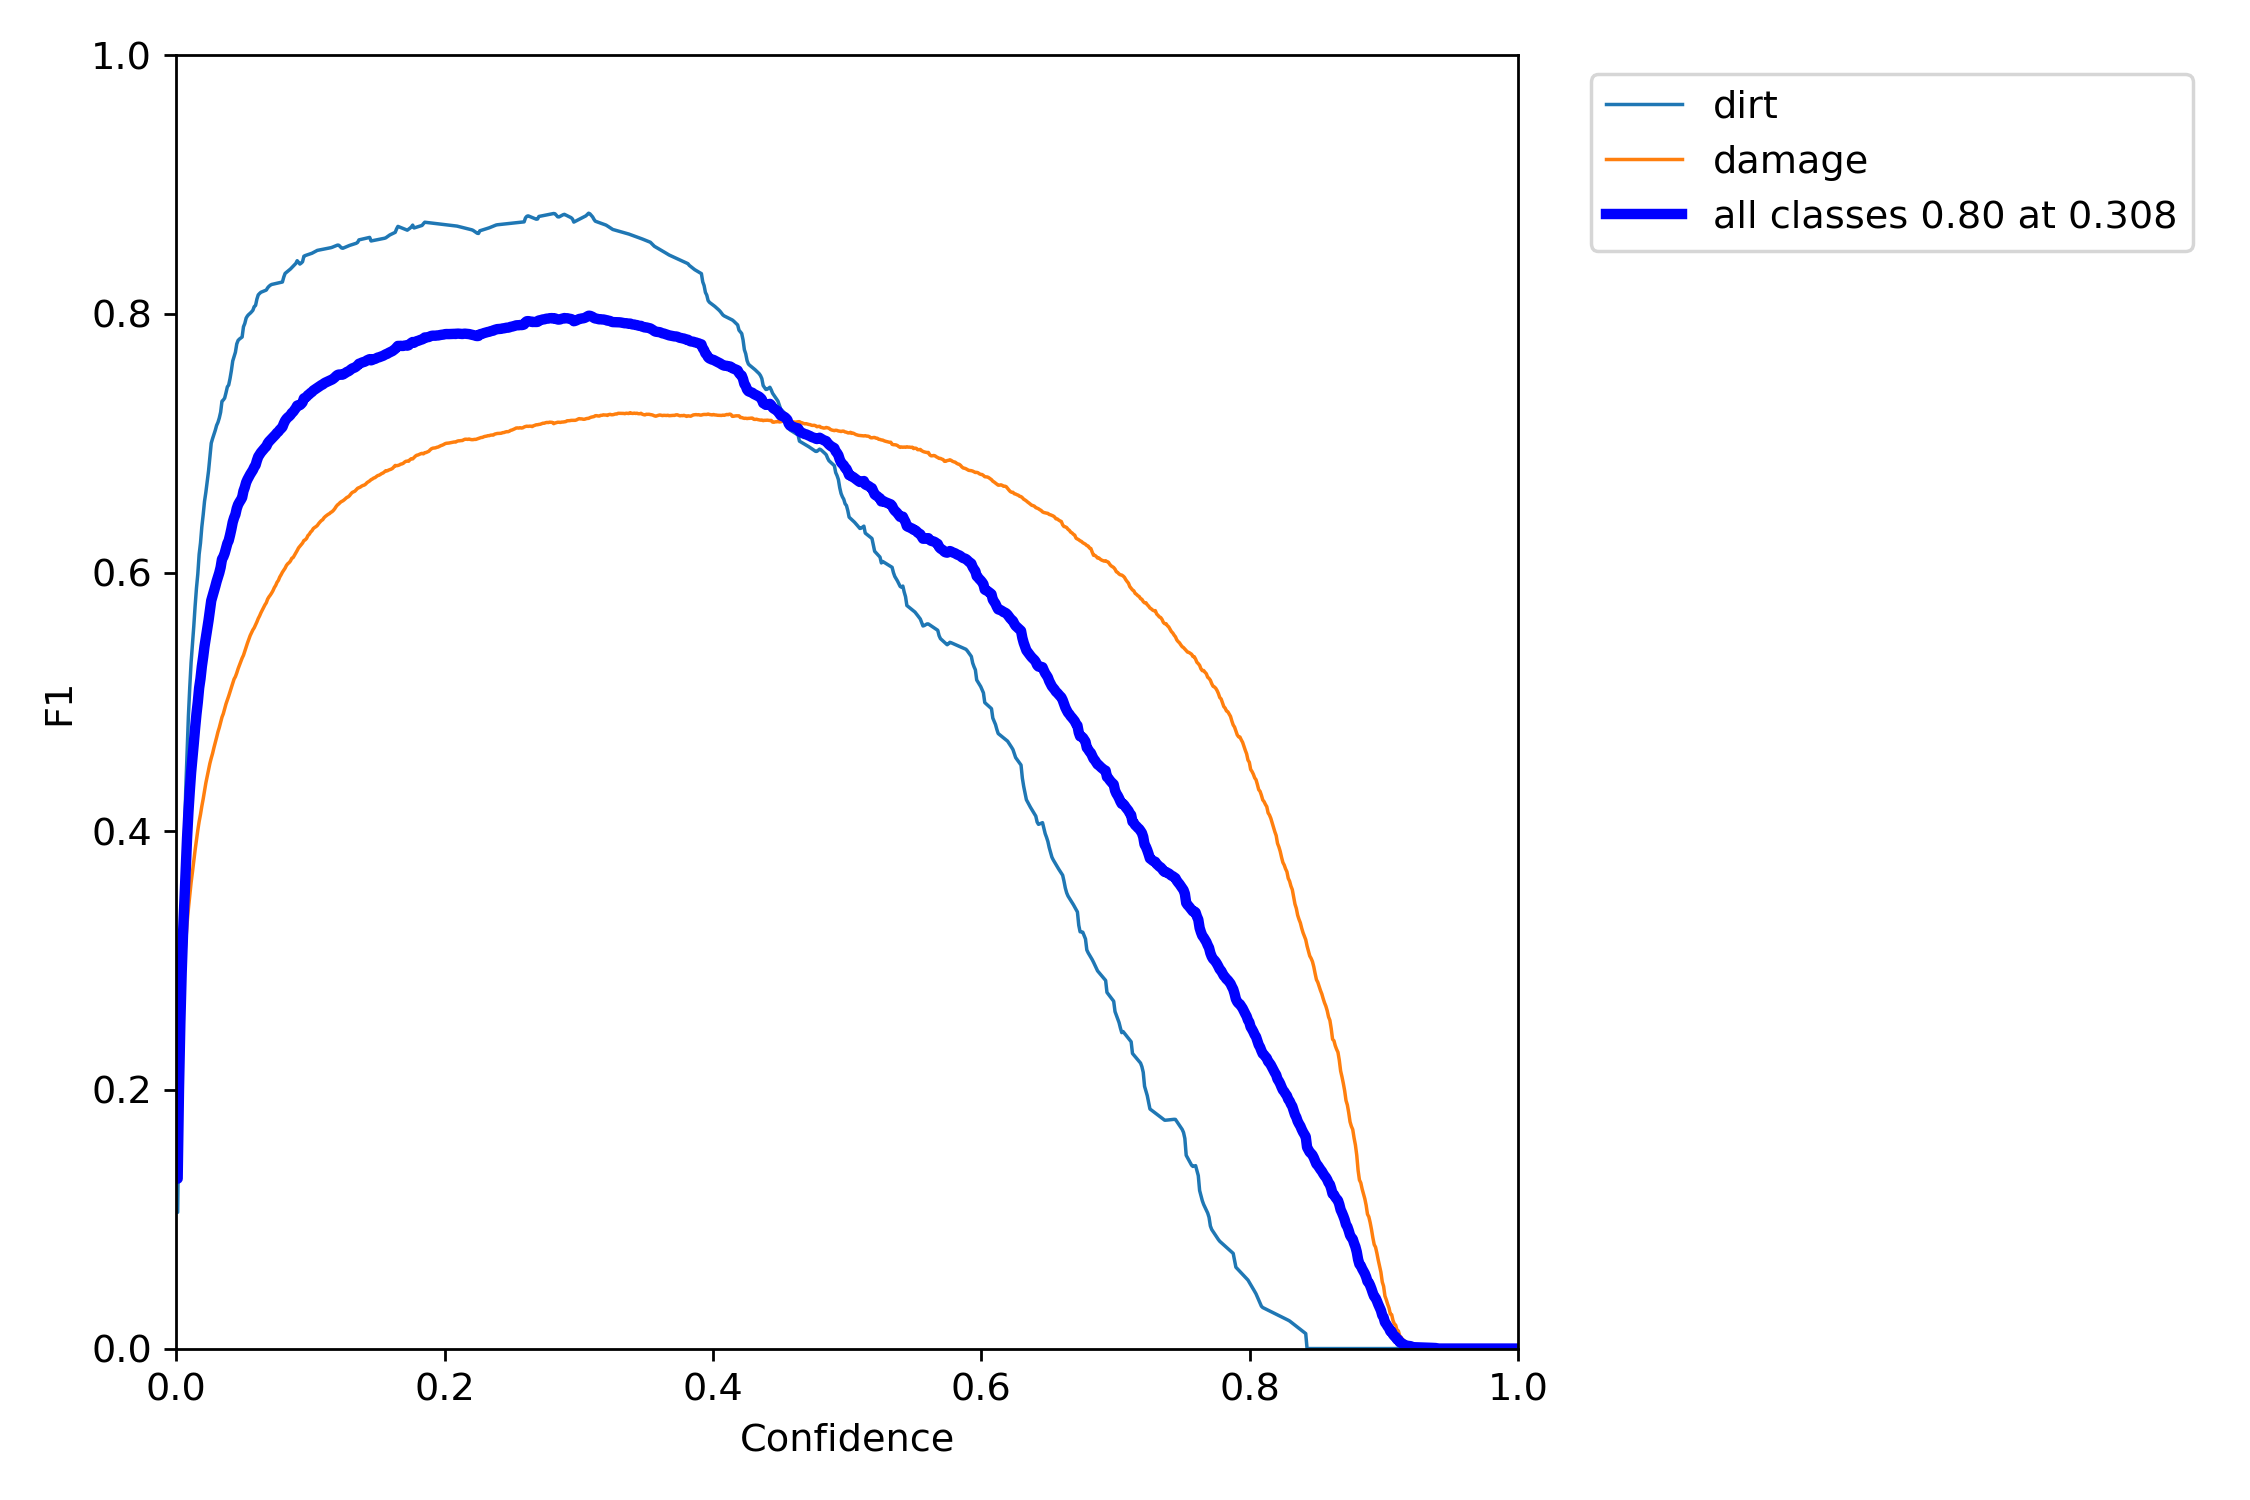
\includegraphics[width=8cm]{Images/YOLOv5m/F1_curve.png}
    \caption{F1-Curve}
\end{figure}
\begin{figure}[H]
    \centering
    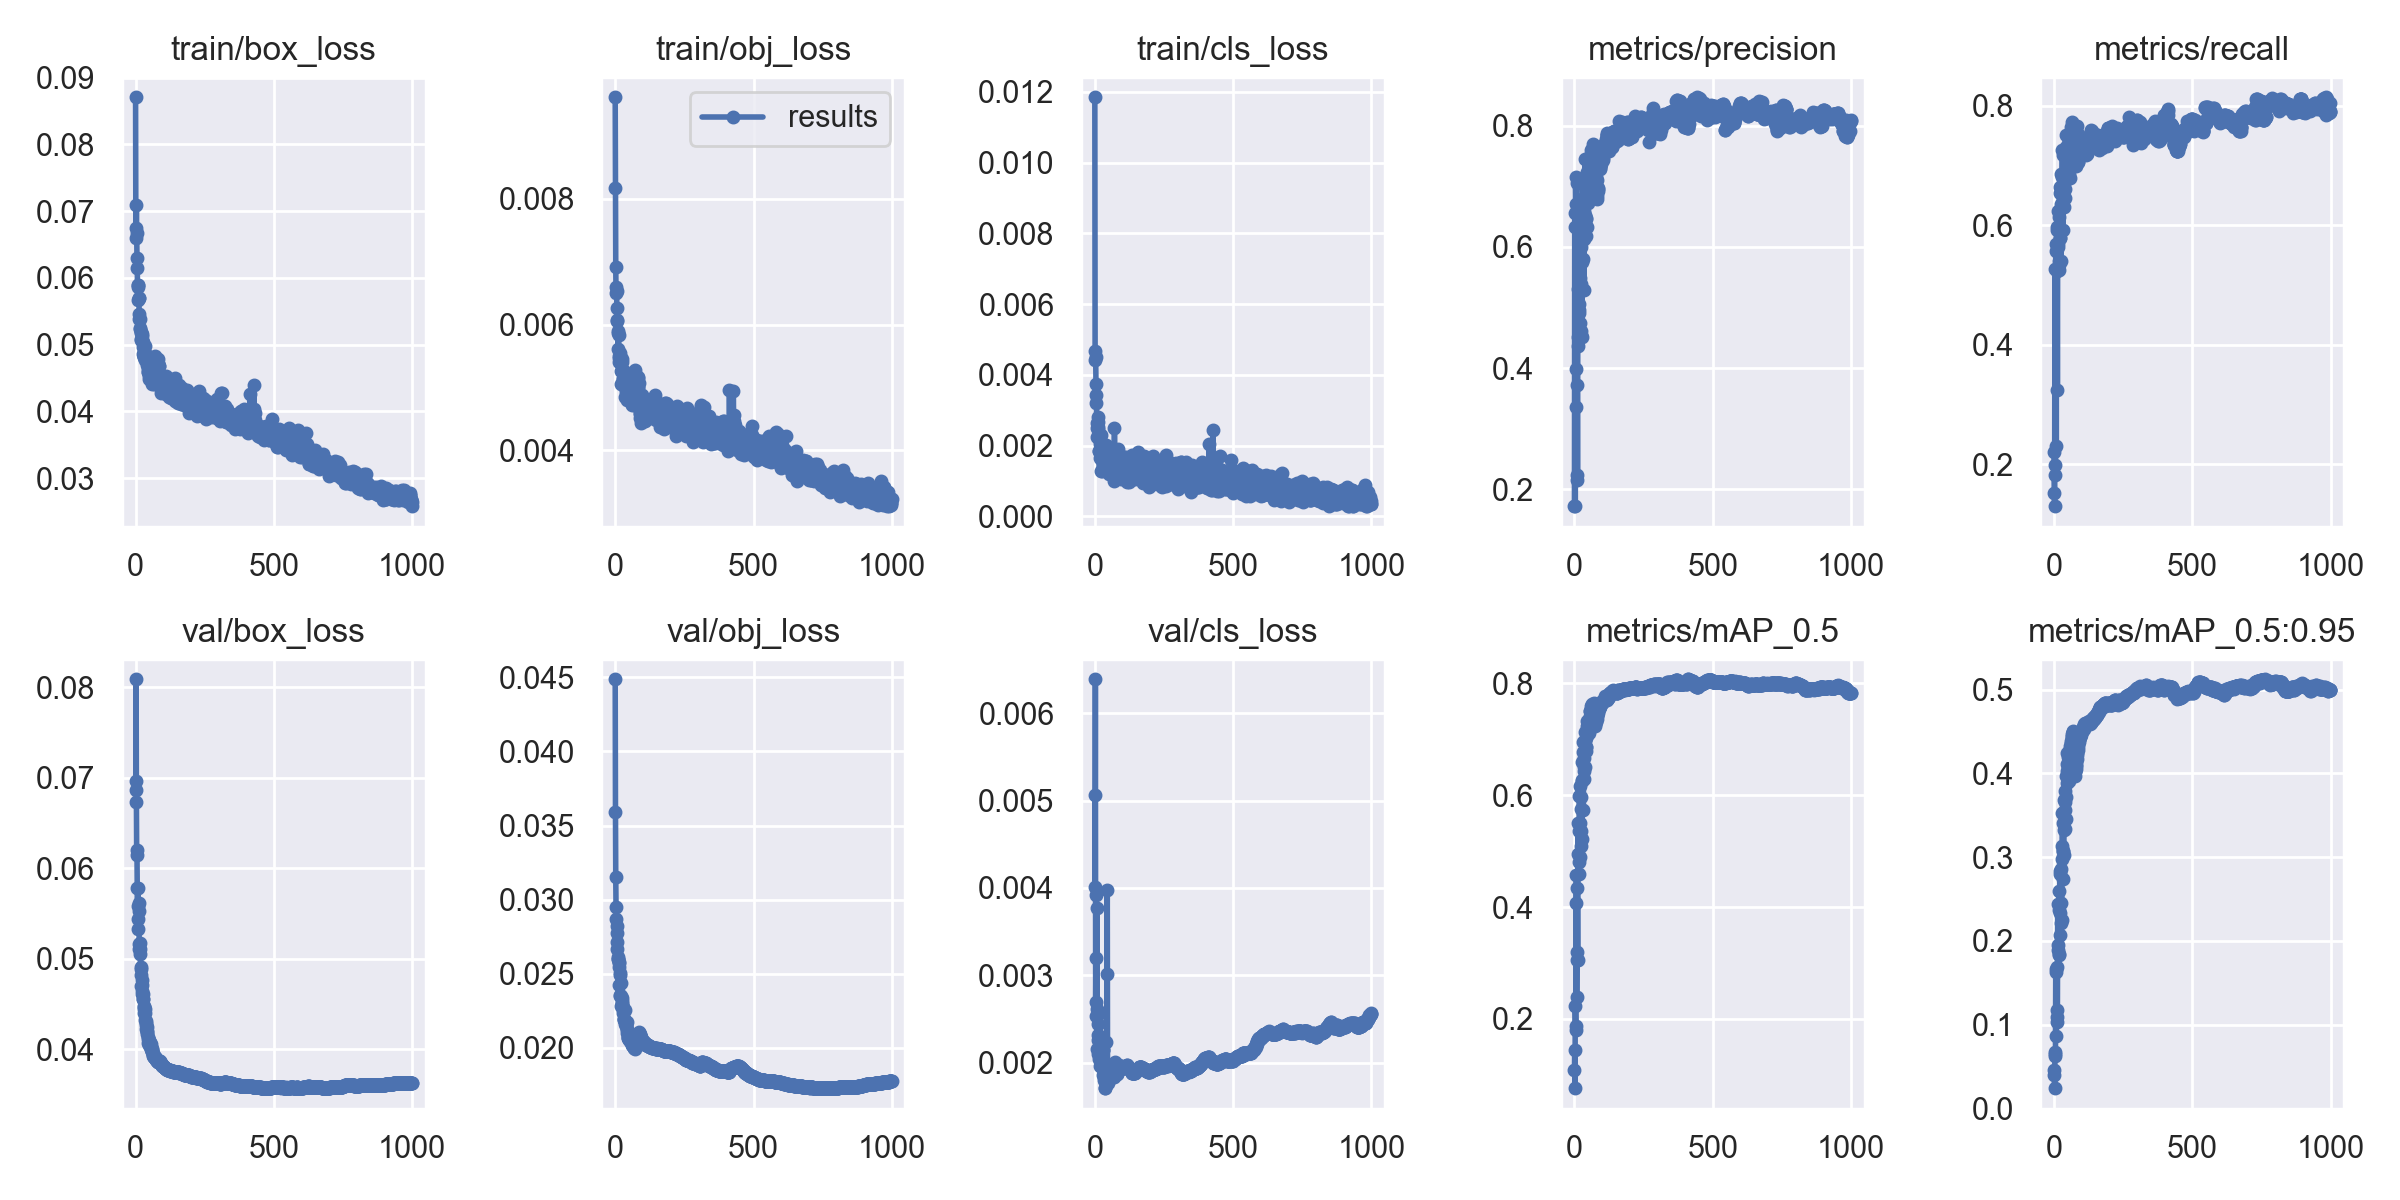
\includegraphics[width=8cm]{Images/YOLOv5m/results.png}
    \caption{Various Results}
\end{figure}
\begin{figure}[H]
    \centering
    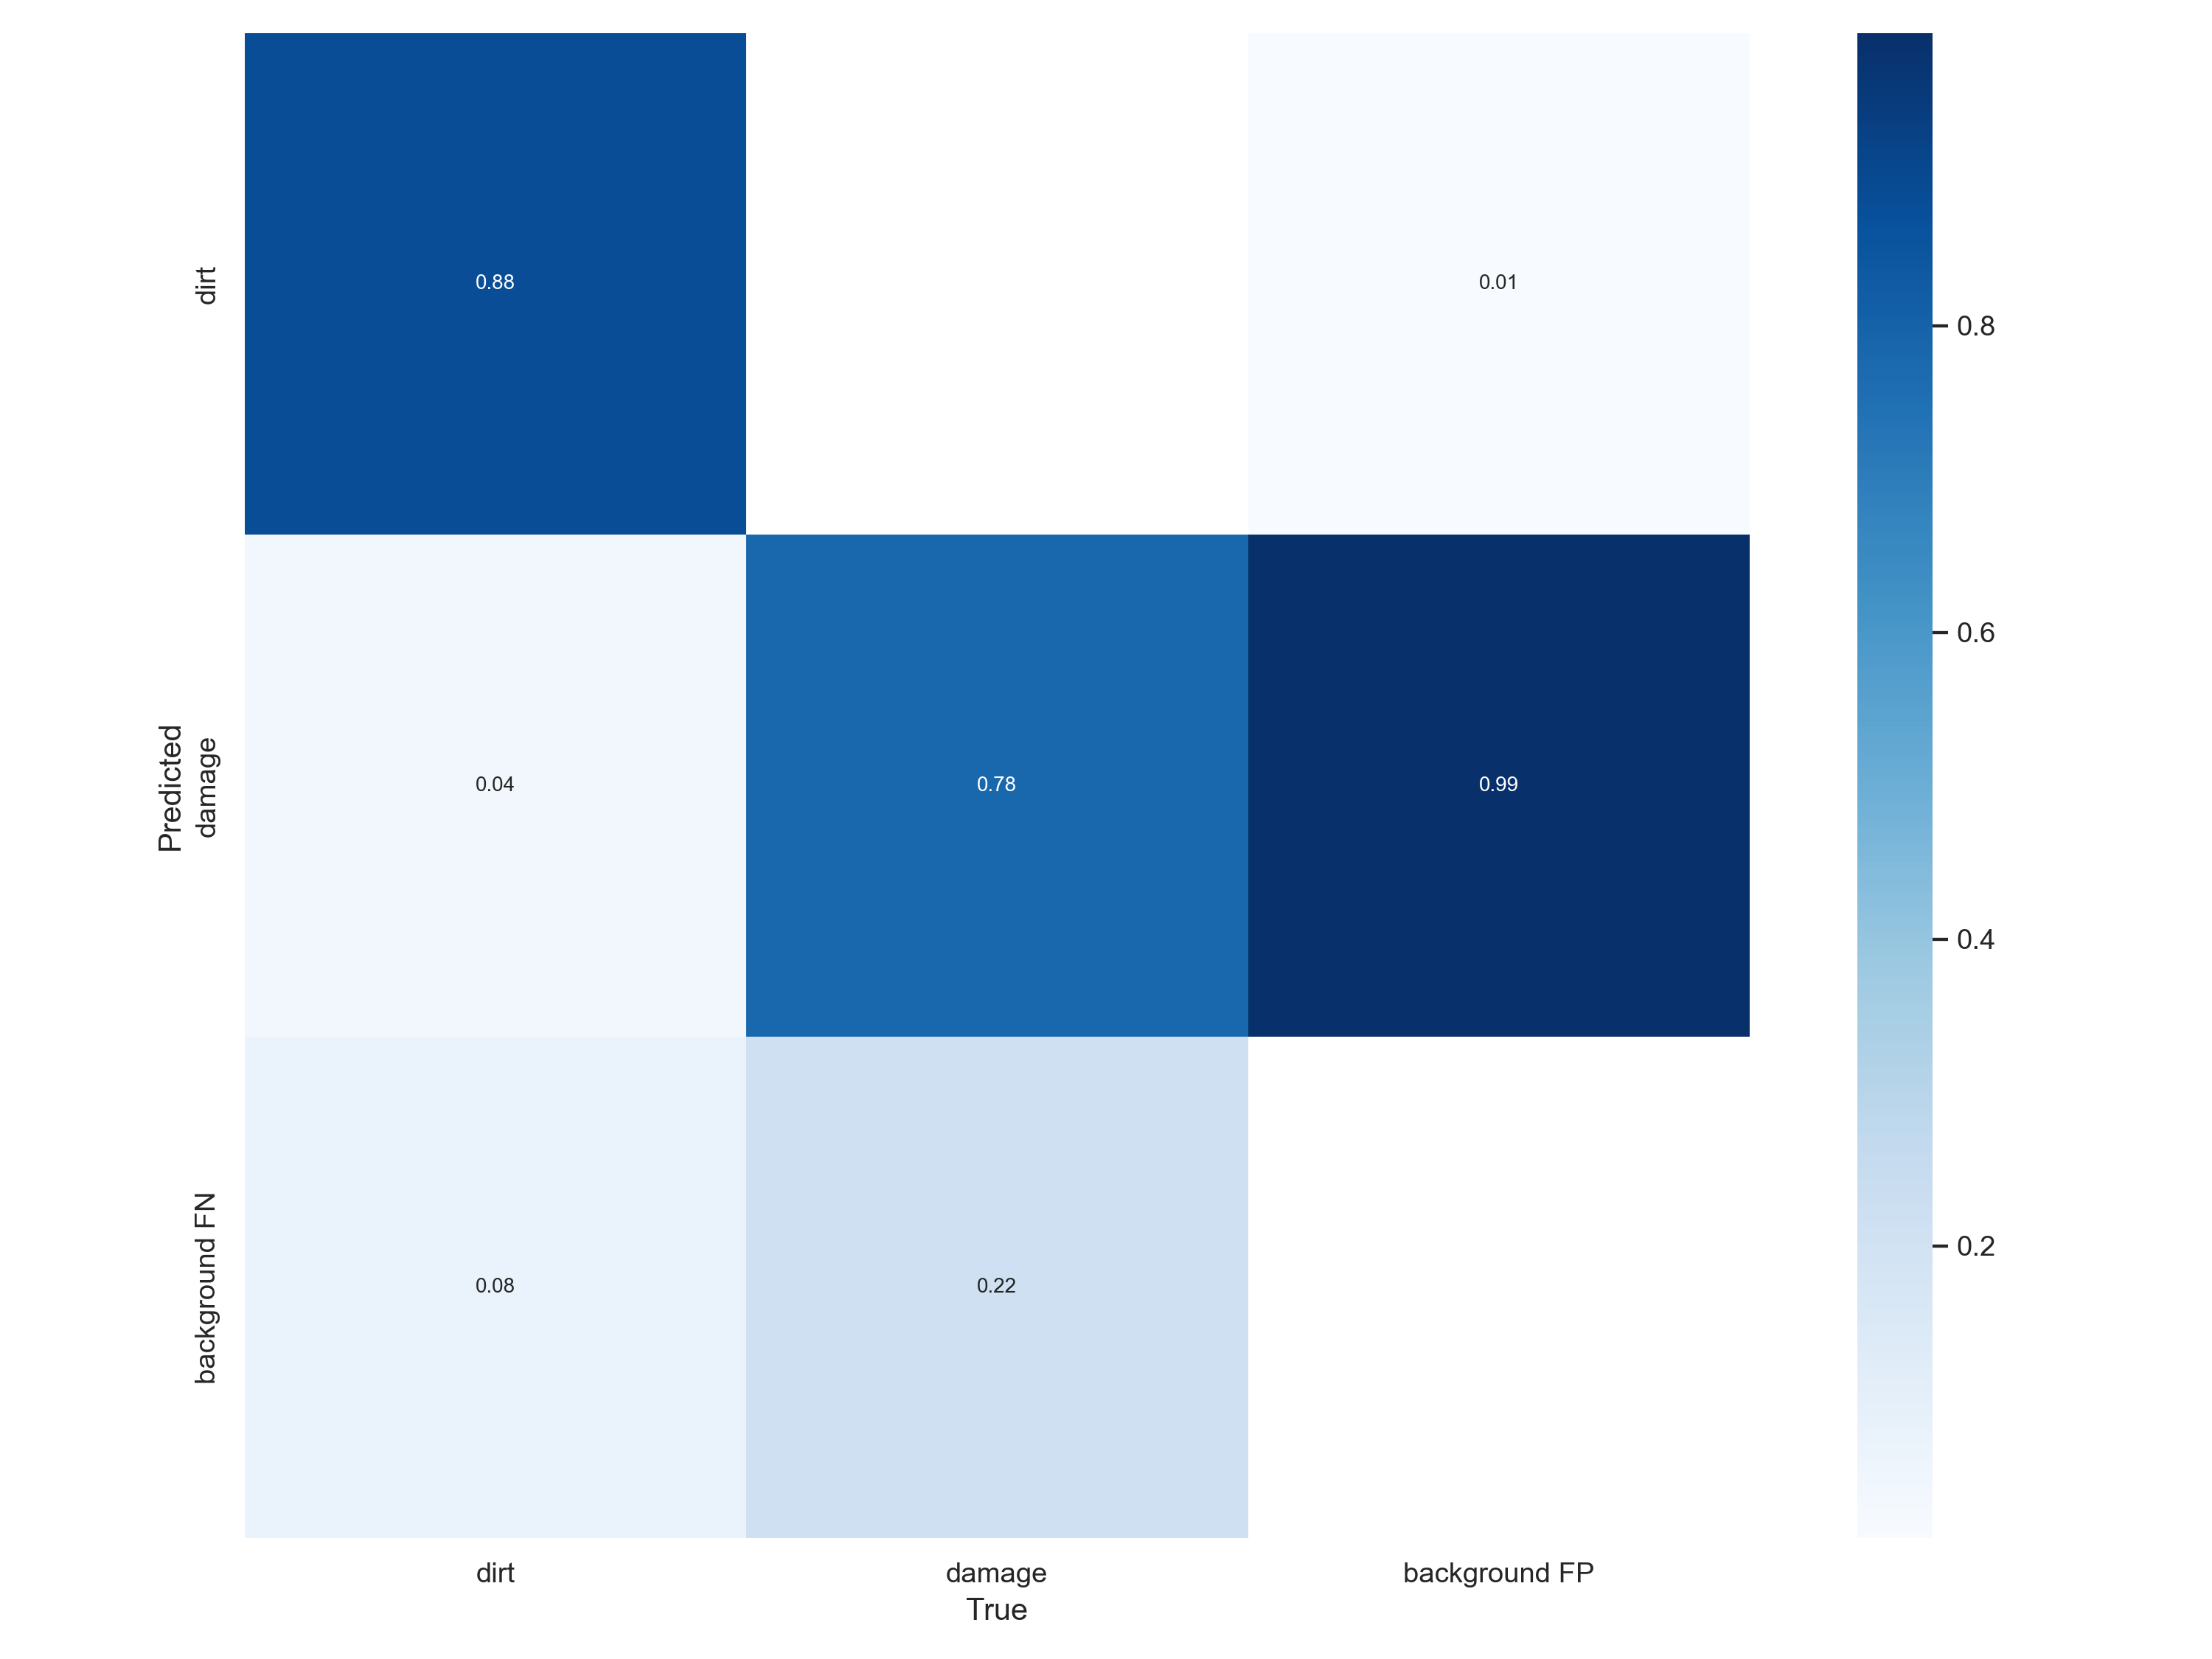
\includegraphics[width=8cm]{Images/Confusion Matrices/mconfusion_matrix.png}
    \caption{Confusion Matrix}
\end{figure}
\subsection{Augmented training batches}
\begin{figure}[H]
    \centering
    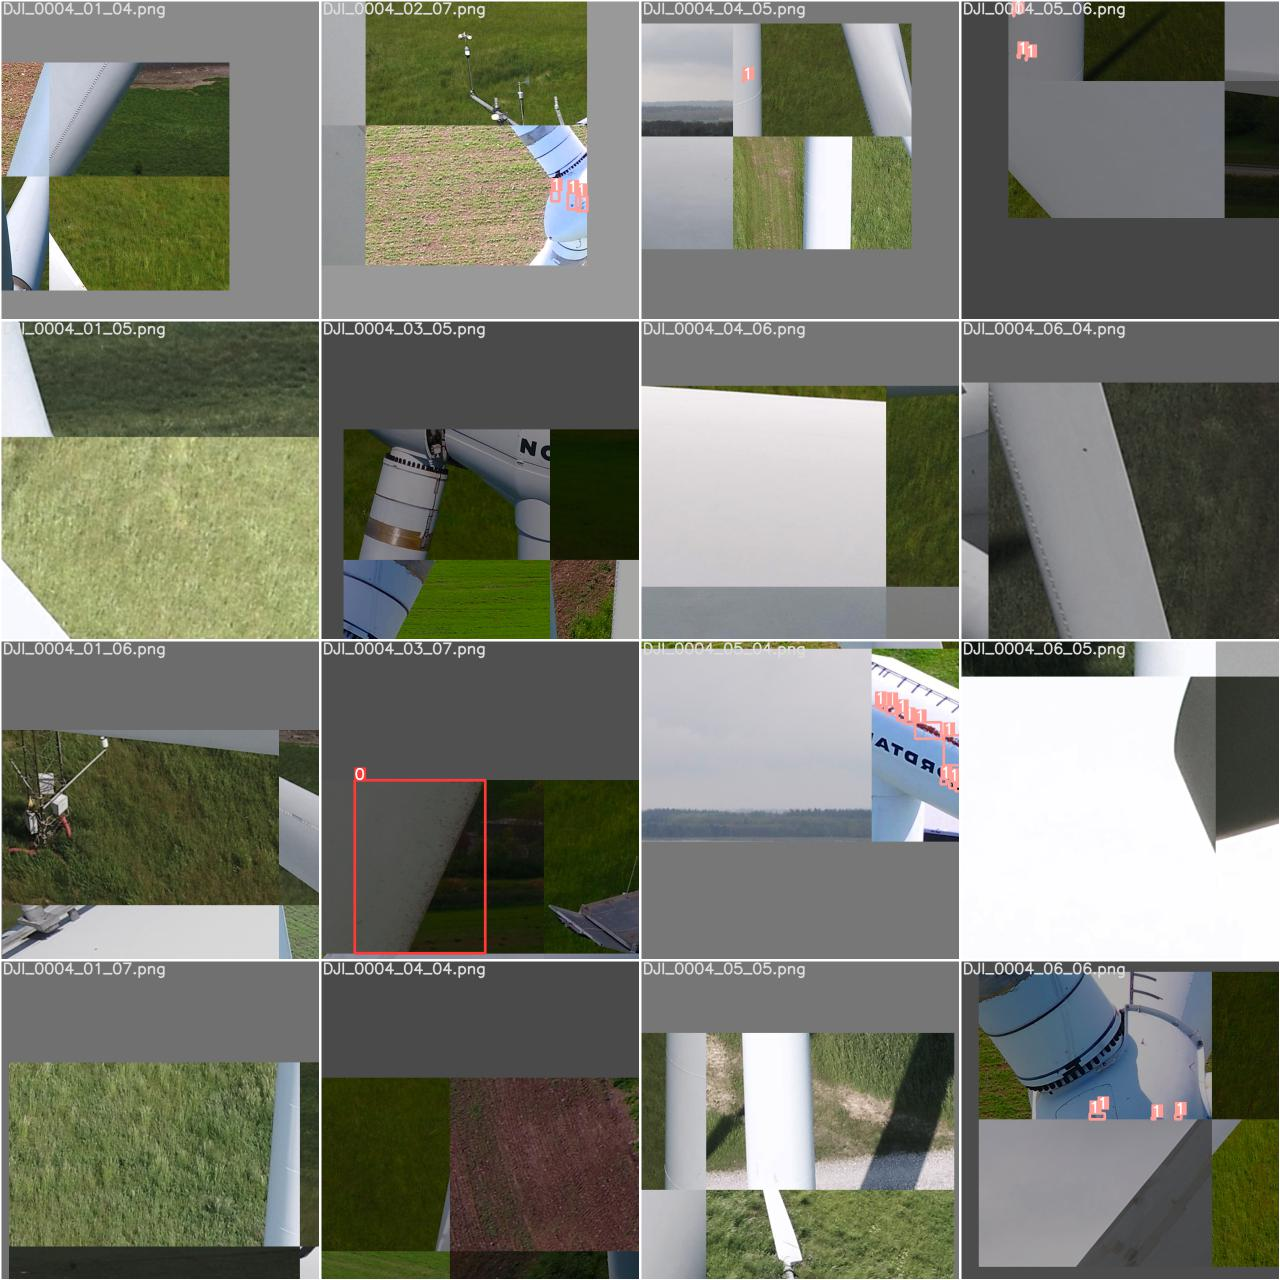
\includegraphics[width=8cm]{Images/YOLOv5m/train_batch0.jpg}
    \caption{Training Batch 0}
\end{figure}
\begin{figure}[H]
    \centering
    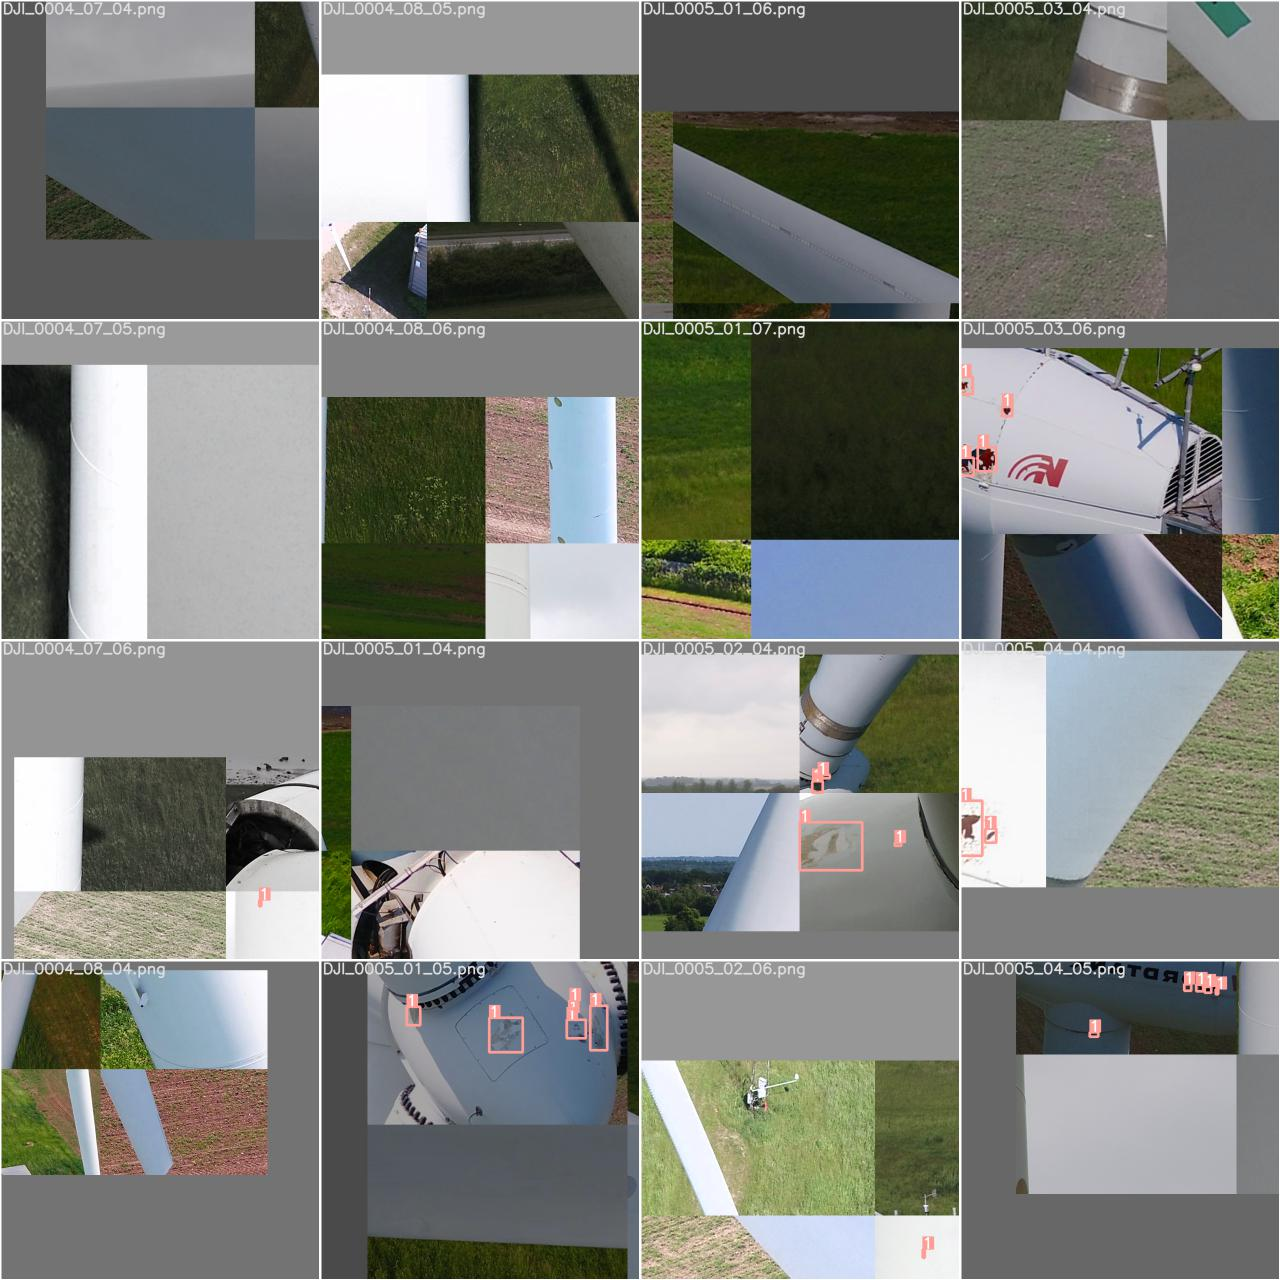
\includegraphics[width=8cm]{Images/YOLOv5m/train_batch1.jpg}
    \caption{Training Batch 1}
\end{figure}
\begin{figure}[H]
    \centering
    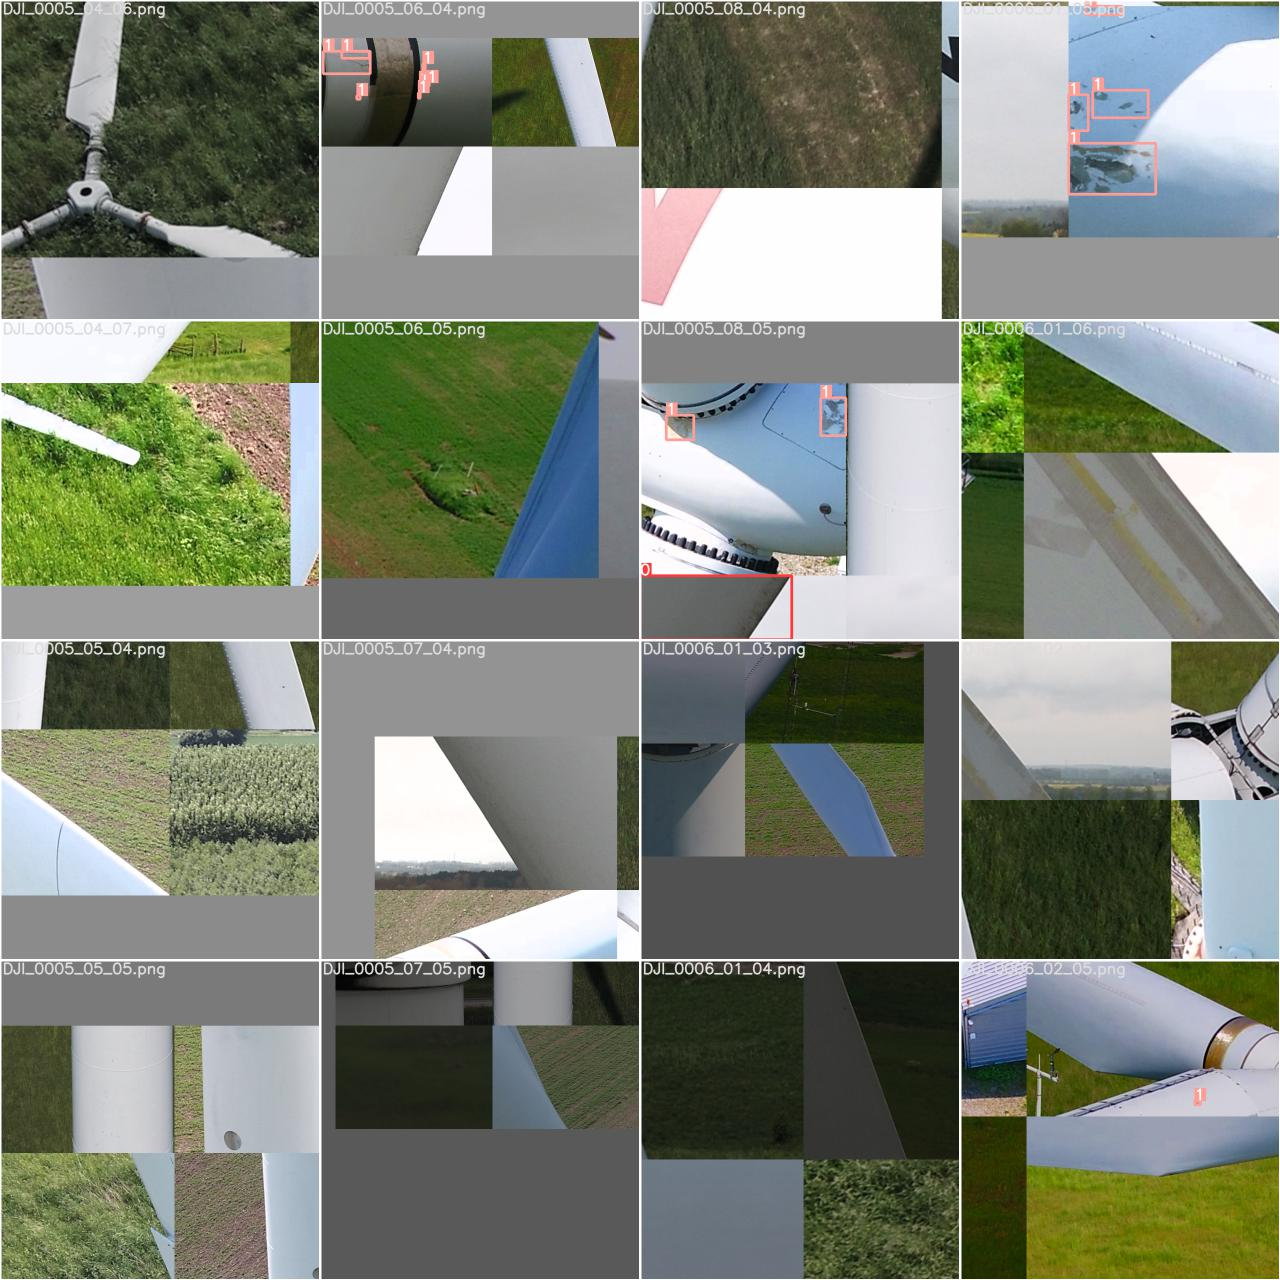
\includegraphics[width=8cm]{Images/YOLOv5m/train_batch2.jpg}
    \caption{Training Batch 2}
\end{figure}
\subsection{Validation batches}
\begin{figure}[H]
    \centering
    \includegraphics[width=8cm]{Images/YOLOv5m/val_batch0_labels.jpg}
    \caption{Validation Batch 0 True Bounding Boxes}
\end{figure}
\begin{figure}[H]
    \centering
    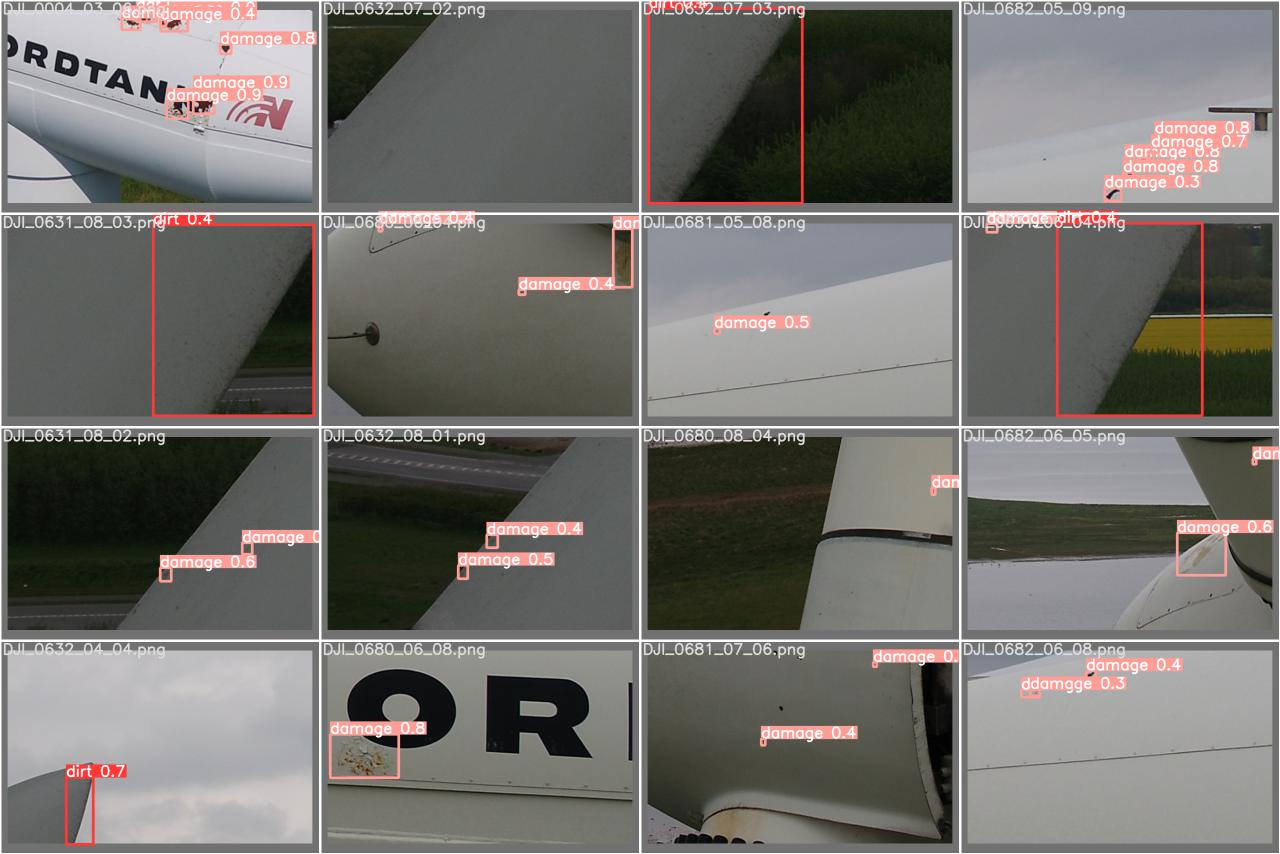
\includegraphics[width=8cm]{Images/YOLOv5m/val_batch0_pred.jpg}
    \caption{Validation Batch 0 Predictions}
\end{figure}
\begin{figure}[H]
    \centering
    \includegraphics[width=8cm]{Images/YOLOv5m/val_batch1_labels.jpg}
    \caption{Validation Batch 1 True Bounding Boxes}
\end{figure}
\begin{figure}[H]
    \centering
    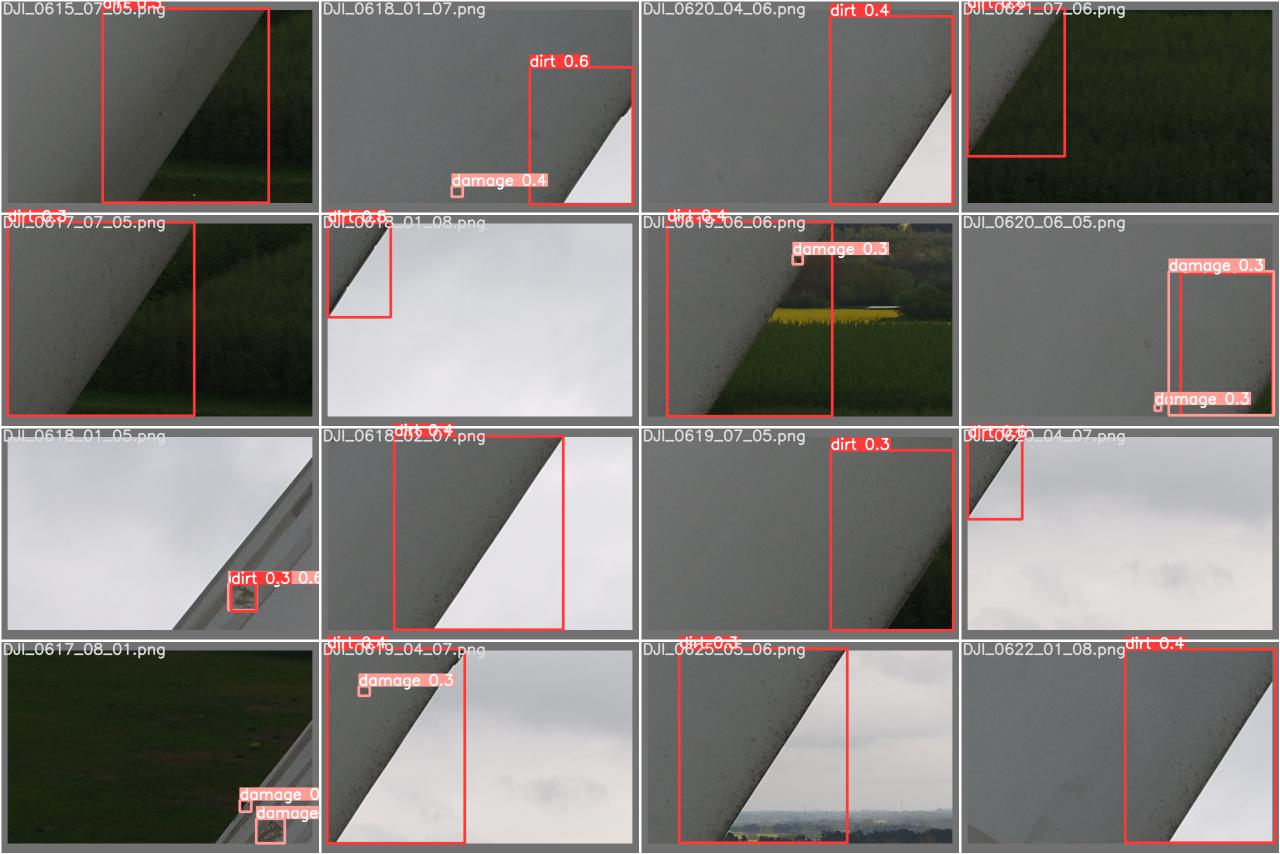
\includegraphics[width=8cm]{Images/YOLOv5m/val_batch1_pred.jpg}
    \caption{Validation Batch 1 Predictions}
\end{figure}
\begin{figure}[H]
    \centering
    \includegraphics[width=8cm]{Images/YOLOv5m/val_batch2_labels.jpg}
    \caption{Validation Batch 2 True Bounding Boxes}
\end{figure}
\begin{figure}[H]
    \centering
    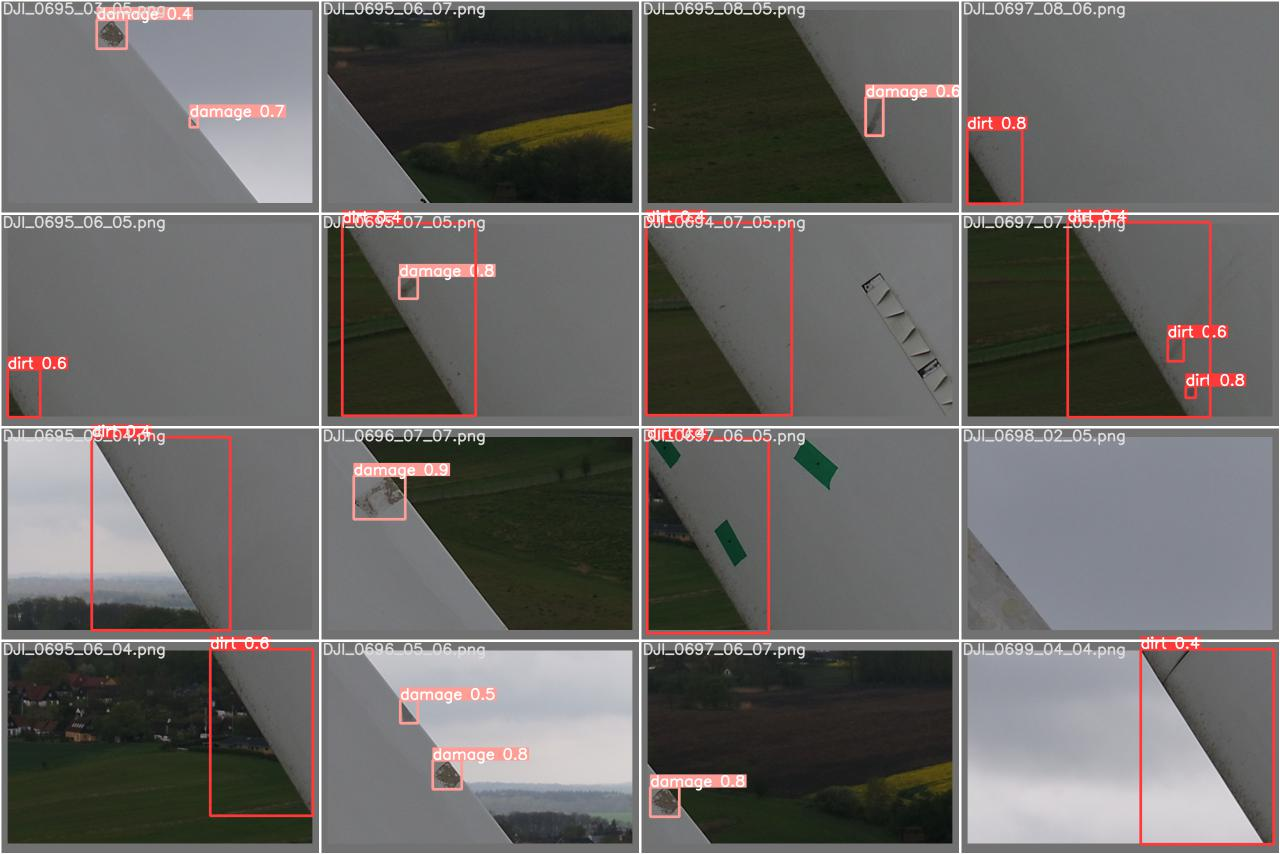
\includegraphics[width=8cm]{Images/YOLOv5m/val_batch2_pred.jpg}
    \caption{Validation Batch 2 Predictions}
\end{figure}
\cleardoublepage
\subsection{YOLOv5s}

\begin{figure}[H]
    \centering
    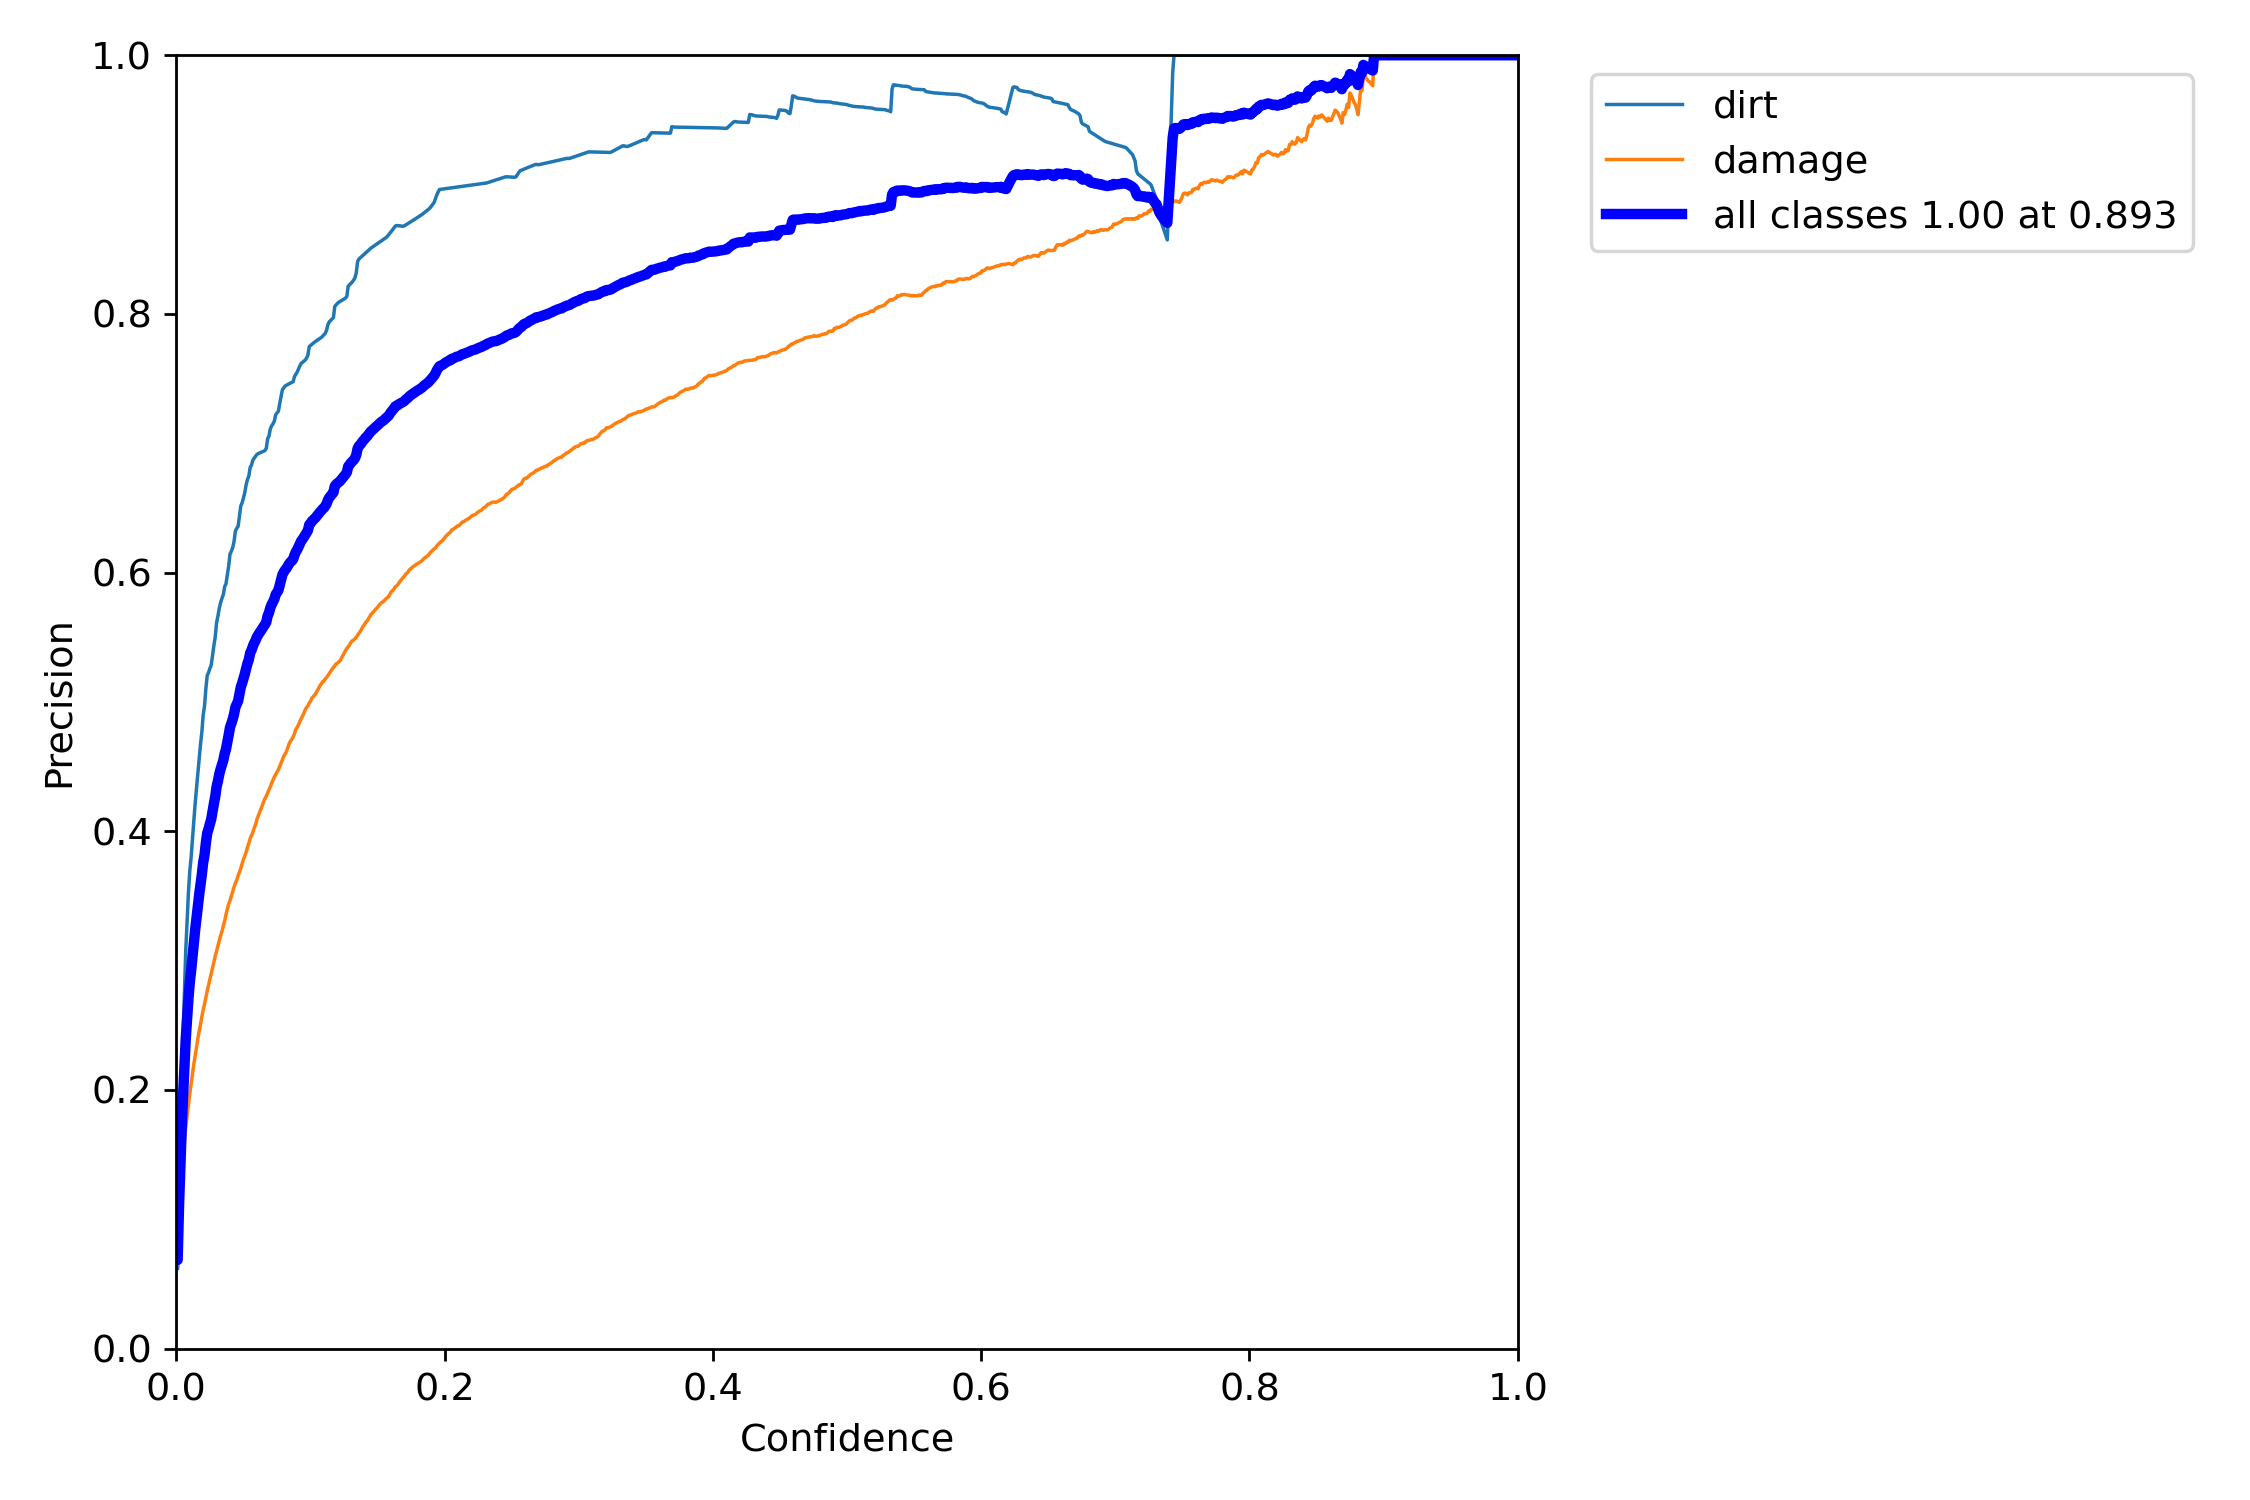
\includegraphics[width=8cm]{Images/YOLOv5s/P_curve.png}
    \caption{Precision-Curve}
\end{figure}
\begin{figure}[H]
    \centering
    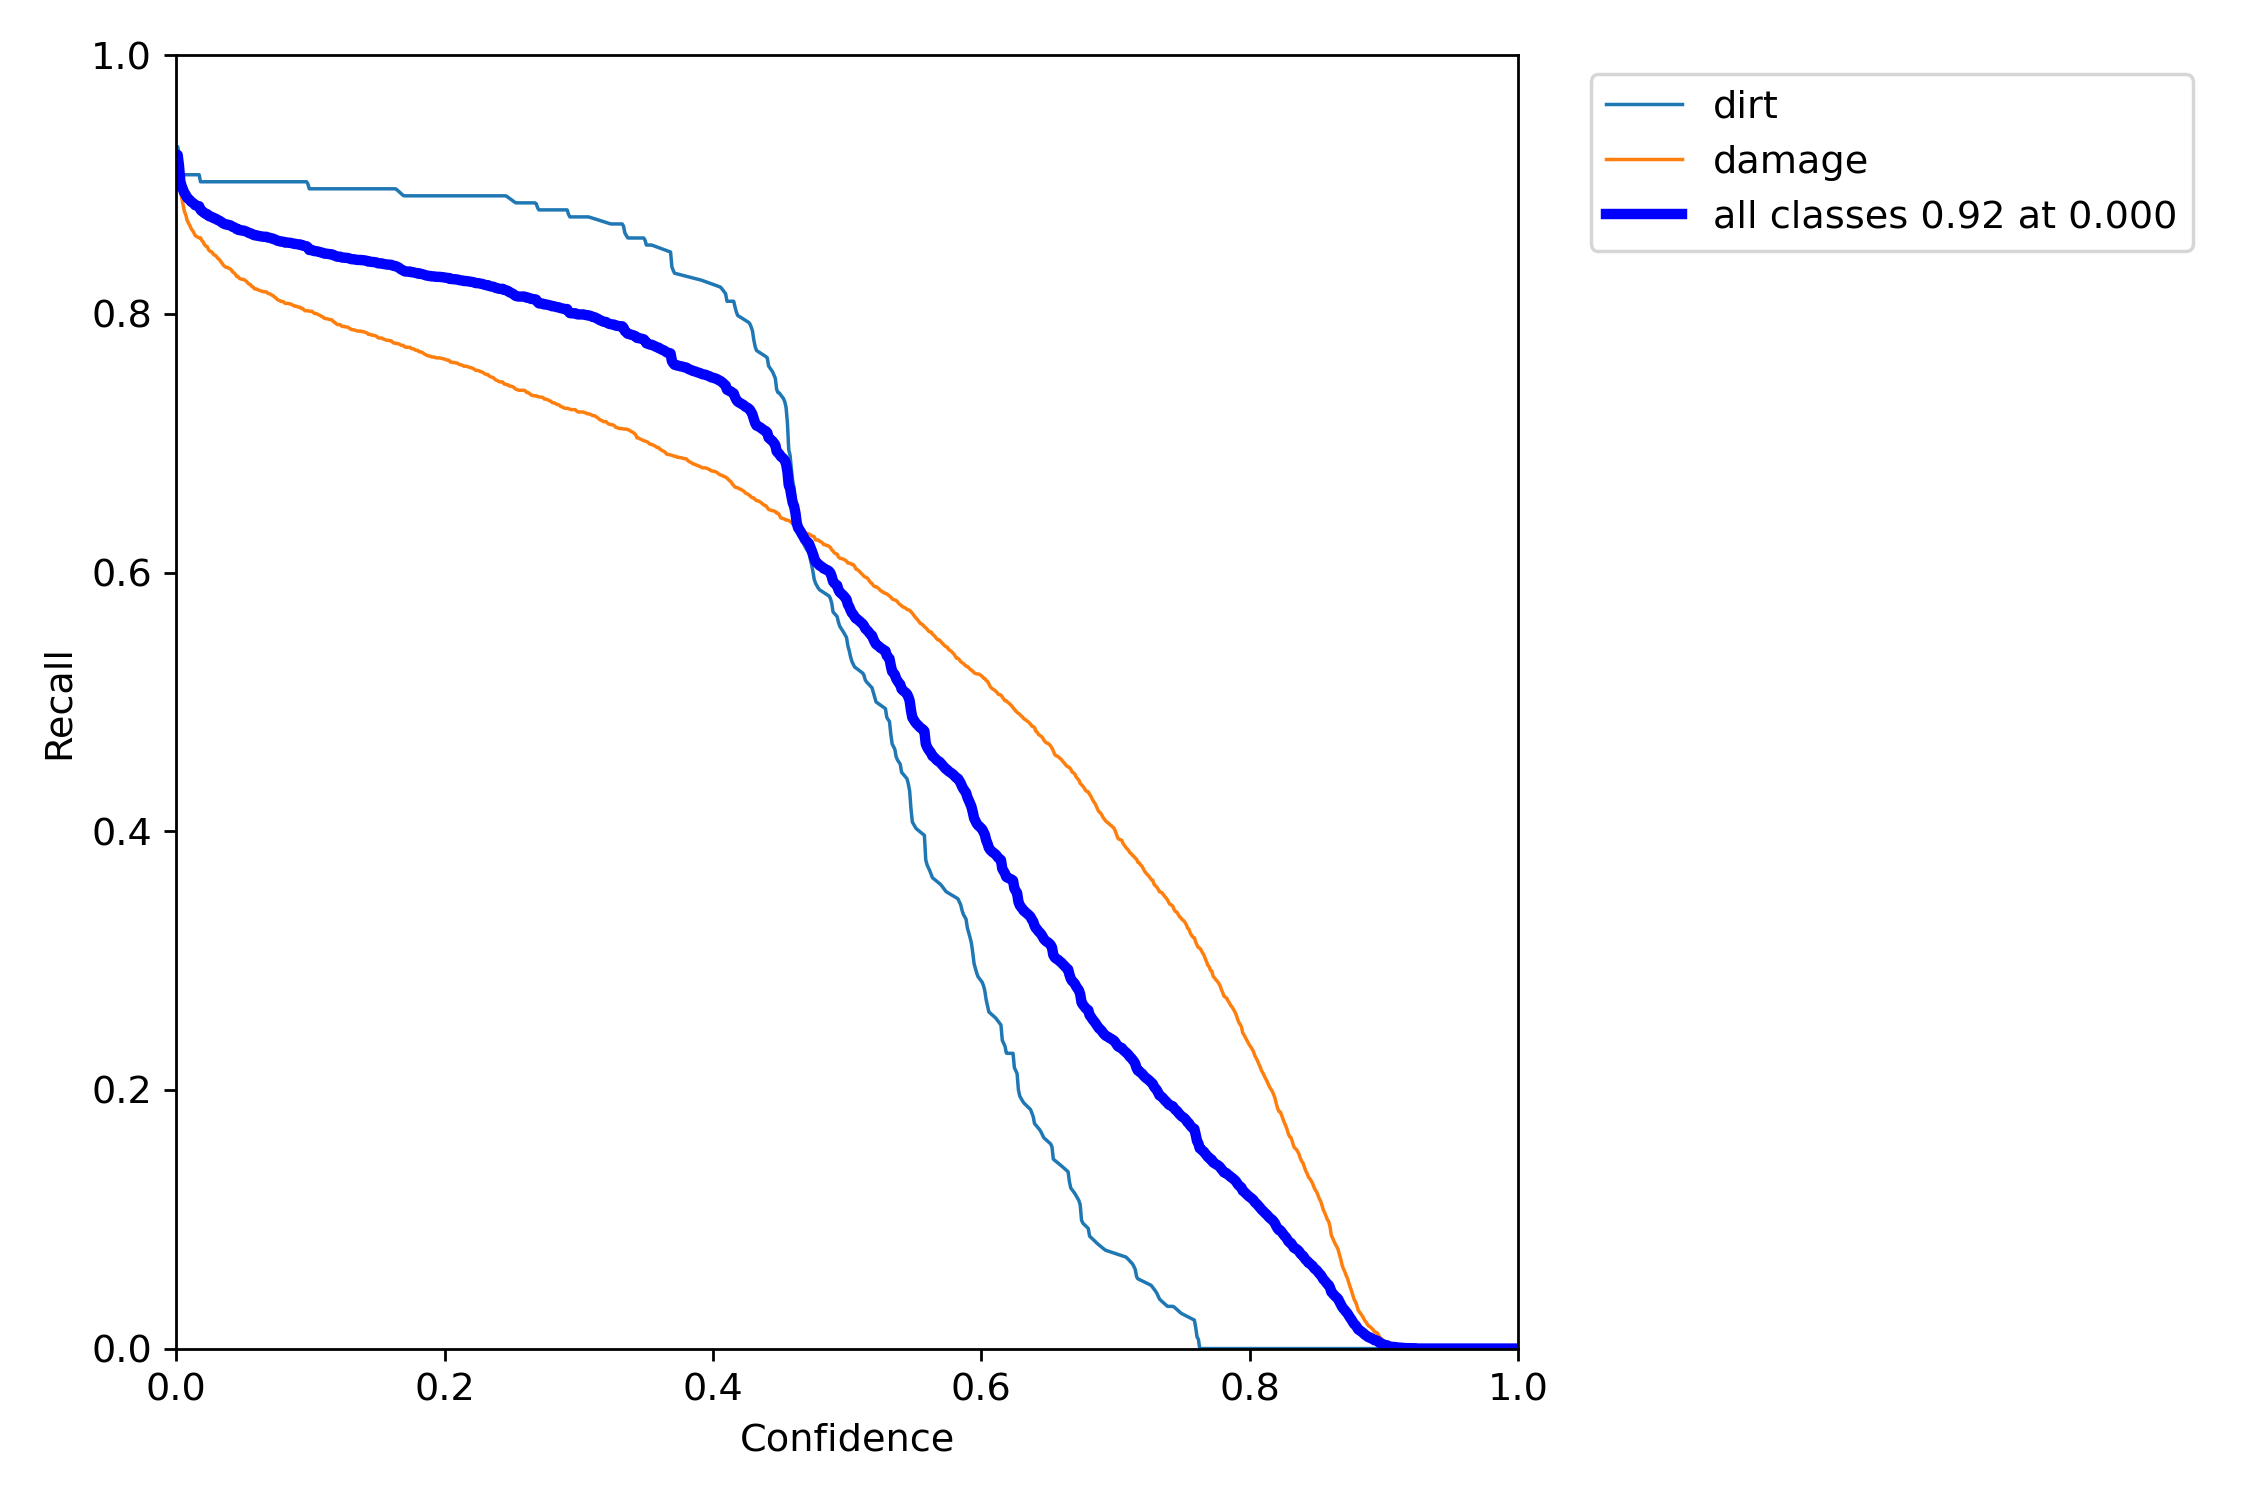
\includegraphics[width=8cm]{Images/YOLOv5s/R_curve.png}
    \caption{Recall-Curve}
\end{figure}
\begin{figure}[H]
    \centering
    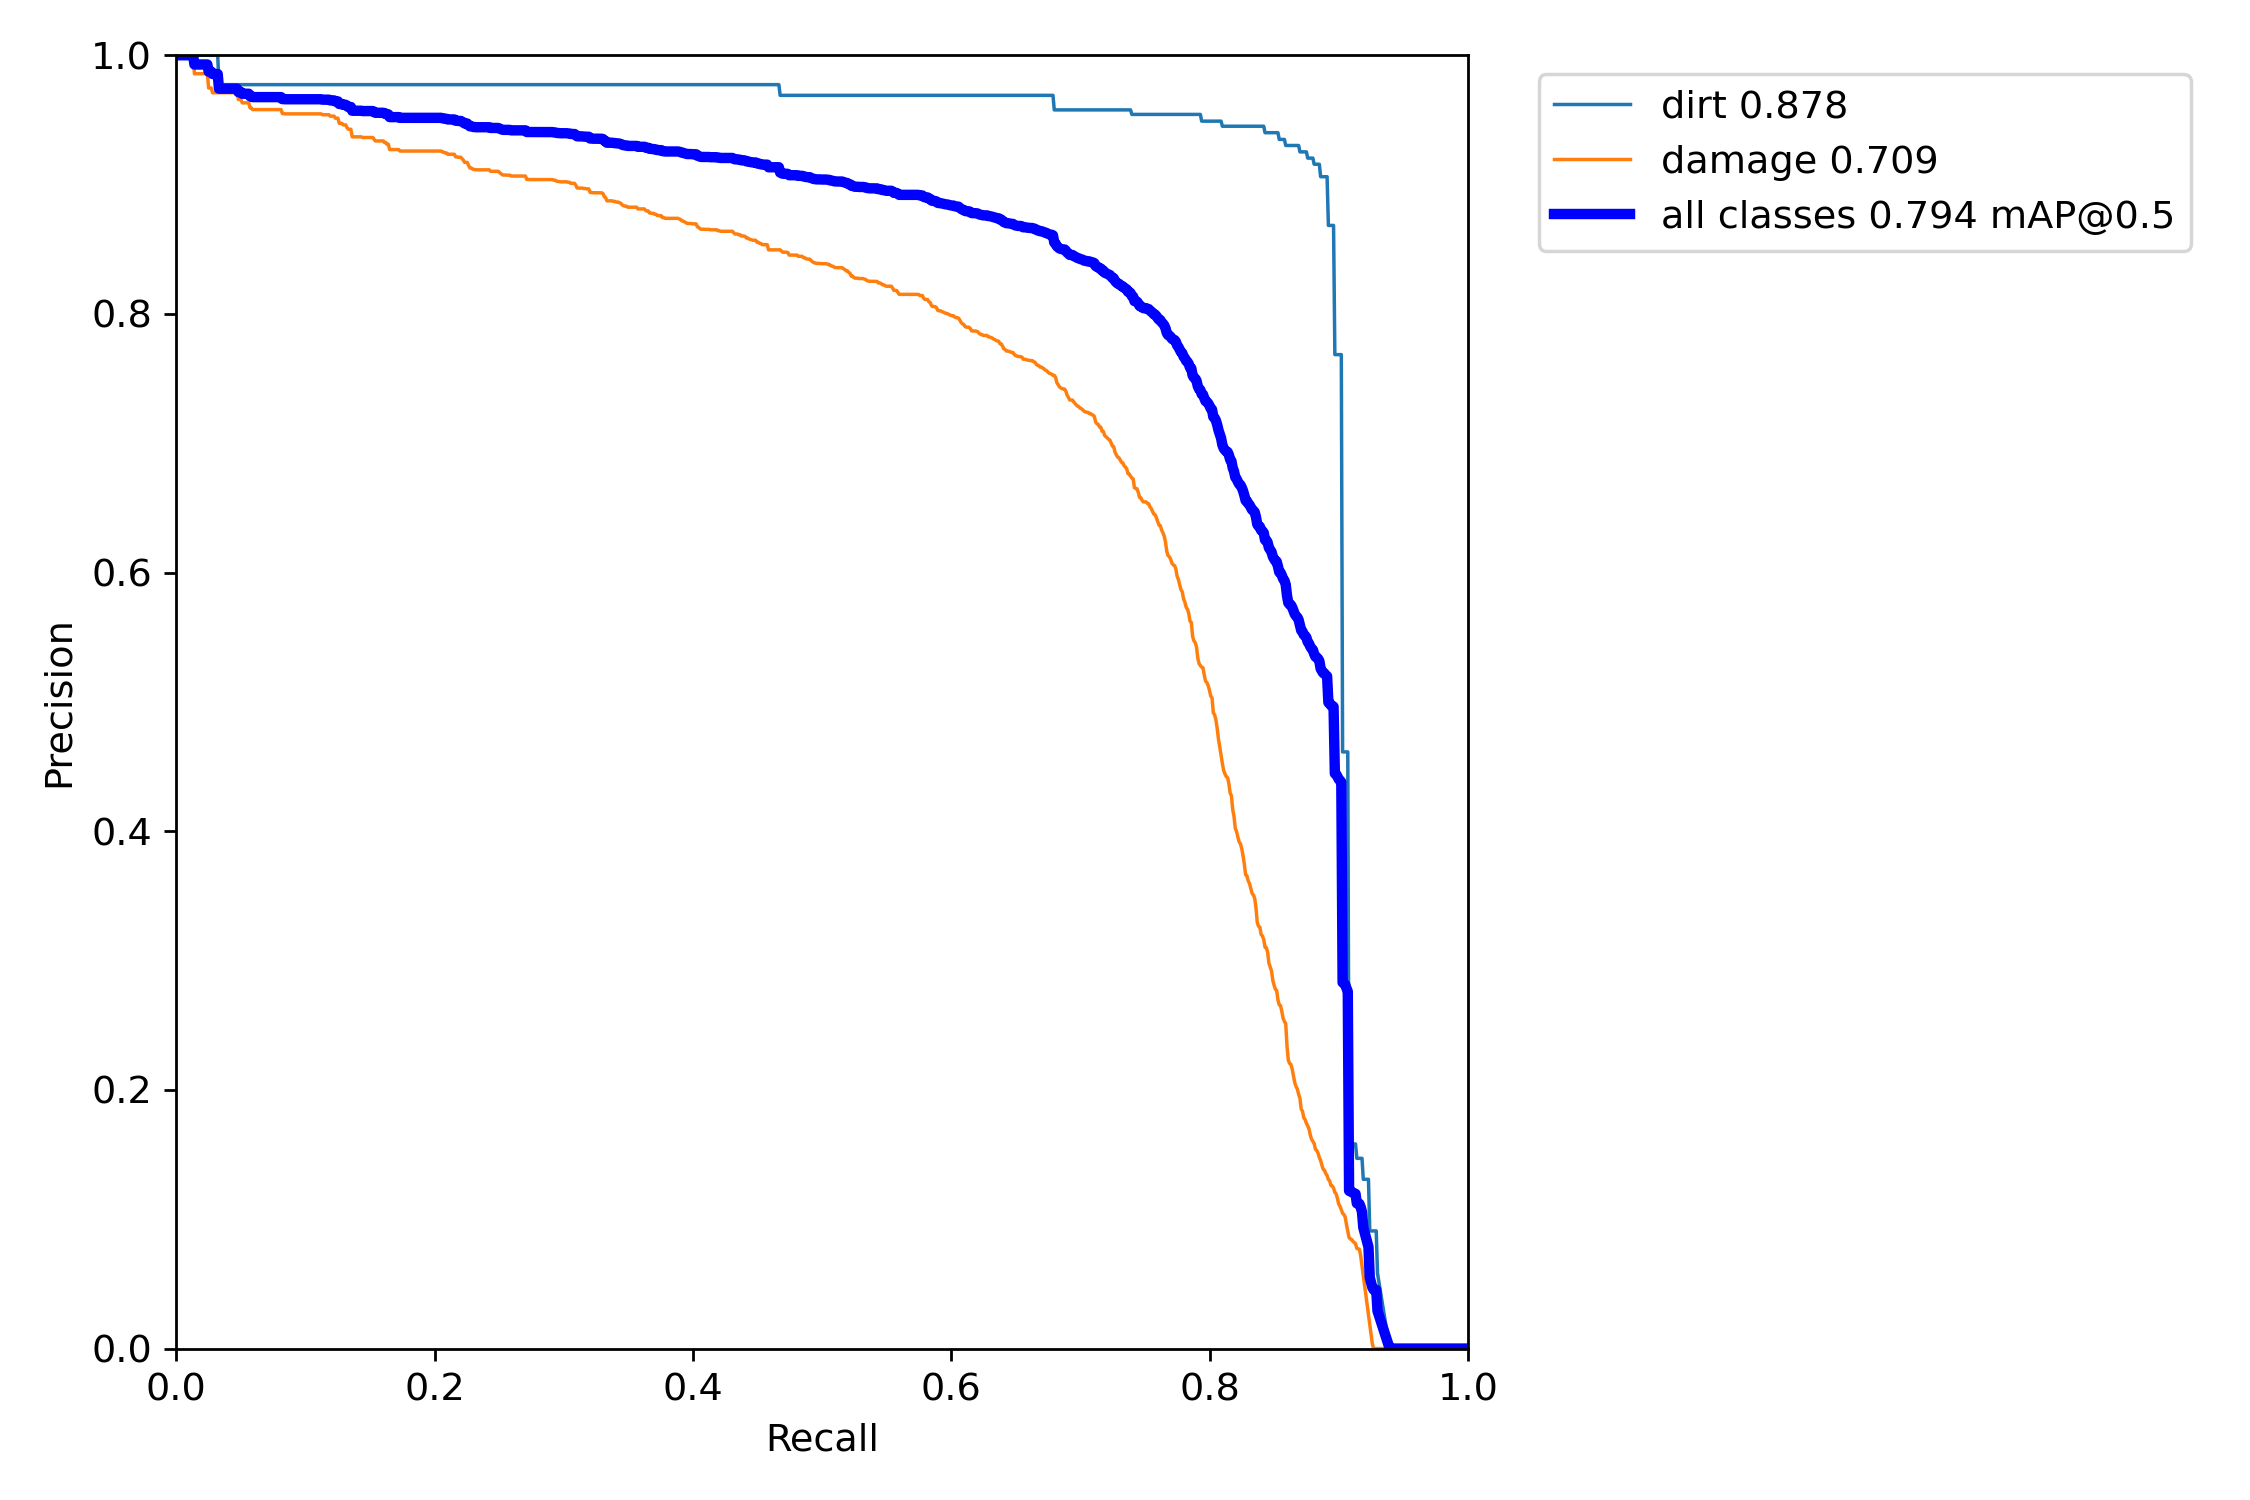
\includegraphics[width=8cm]{Images/YOLOv5s/PR_curve.png}
    \caption{PR-Curve}
\end{figure}
\begin{figure}[H]
    \centering
    \includegraphics[width=8cm]{Images/YOLOv5s/F1_curve.png}
    \caption{F1-Curve}
\end{figure}
\begin{figure}[H]
    \centering
    \includegraphics[width=8cm]{Images/YOLOv5s/results.png}
    \caption{Various Results}
\end{figure}

\begin{figure}[H]
    \centering
    \includegraphics[width=8cm]{Images/Confusion Matrices/sconfusion_matrix.png}
    \caption{Confusion Matrix}
\end{figure}
\subsection{Augmented training batches}
\begin{figure}[H]
    \centering
    \includegraphics[width=8cm]{Images/YOLOv5s/train_batch0.jpg}
    \caption{Training Batch 0}
\end{figure}
\begin{figure}[H]
    \centering
    \includegraphics[width=8cm]{Images/YOLOv5s/train_batch1.jpg}
    \caption{Training Batch 1}
\end{figure}
\begin{figure}[H]
    \centering
    \includegraphics[width=8cm]{Images/YOLOv5s/train_batch2.jpg}
    \caption{Training Batch 2}
\end{figure}
\subsection{Validation batches}
\begin{figure}[H]
    \centering
    \includegraphics[width=8cm]{Images/YOLOv5s/val_batch0_labels.jpg}
    \caption{Validation Batch 0 True Bounding Boxes}
\end{figure}
\begin{figure}[H]
    \centering
    \includegraphics[width=8cm]{Images/YOLOv5s/val_batch0_pred.jpg}
    \caption{Validation Batch 0 Predictions}
\end{figure}
\begin{figure}[H]
    \centering
    \includegraphics[width=8cm]{Images/YOLOv5s/val_batch1_labels.jpg}
    \caption{Validation Batch 1 True Bounding Boxes}
\end{figure}
\begin{figure}[H]
    \centering
    \includegraphics[width=8cm]{Images/YOLOv5s/val_batch1_pred.jpg}
    \caption{Validation Batch 1 Predictions}
\end{figure}
\begin{figure}[H]
    \centering
    \includegraphics[width=8cm]{Images/YOLOv5s/val_batch2_labels.jpg}
    \caption{Validation Batch 2 True Bounding Boxes}
\end{figure}
\begin{figure}[H]
    \centering
    \includegraphics[width=8cm]{Images/YOLOv5s/val_batch2_pred.jpg}
    \caption{Validation Batch 2 Predictions}
\end{figure}
\cleardoublepage
\subsection{Faster R-CNN}
\begin{figure}[H]
    \centering
    \includegraphics[width=8cm]{Images/Faster/AP75.png}
    \caption{mAP@.75}
\end{figure}
\begin{figure}[H]
    \centering
    \includegraphics[width=8cm]{Images/Faster/APdamage.png}
    \caption{AP of Damage Class}
\end{figure}
\begin{figure}[H]
    \centering
    \includegraphics[width=8cm]{Images/Faster/APdirt.png}
    \caption{AP of Dirt Class}
\end{figure}
\begin{figure}[H]
    \centering
    \includegraphics[width=8cm]{Images/Faster/APL.png}
    \caption{AP of large instances}
\end{figure}
\begin{figure}[H]
    \centering
    \includegraphics[width=8cm]{Images/Faster/APM.png}
    \caption{AP of medium instances}
\end{figure}
\begin{figure}[H]
    \centering
    \includegraphics[width=8cm]{Images/Faster/APS.png}
    \caption{AP of small instances}
\end{figure}
\begin{figure}[H]
    \centering
    \includegraphics[width=8cm]{Images/Faster/TotalLoss.png}
    \caption{Total Loss value over training}
\end{figure}




\end{document}


